%% Define the document style. The thesis stylesheet inherits from 'report'. 
%% I had once made a version inheriting from book. However the two versions are almost 
%% compatible. The main difference is that the other version supported 'parts'.
%% (extended from book) and this does not.
%% IST requires the thesis to be written in Arial or similar. Two arguments allow you 
%% to define the thesis font: 'Helvetica' and 'AvantGarde', which transforms normal font
%% into Helvetica or AvantGarde, respectively... dahhhh!
\documentclass[defaultstyle,10pt,master,Helvetica]{thesis}
%\documentclass[defaultstyle,12pt,phd]{thesis}

%% STYLESHEET SPECIFIC EXTRA COMMANDS (defined in thesis.cls):
%% ------------------------------------------------------------
%% \fancychapter{chaptername) -> Prints a fancier chapter
%% \hline{width} -> use for a replacement of the \hline command
%% \Mark1, \Mark2, \Mark3, ...

%% Defines an additional alphabet... not required in most cases
%% ------------------------------------------------------------
% \DeclareMathAlphabet{\mathpzc}{OT1}{pzc}{m}{it}

%% PACKAGE babel:
%% ---------------
%% The 'babel' package may correct some hyphenisation issues of latex. 
%% However in most situations it is not required.
% \usepackage[english]{babel}

%% PORTUGUESE WRITTEN DOCUMENTS
%% ---------------
%% If you are writting the document in portuguese you will have to use the following 
%% packages and commands:
% \usepackage[portuges]{babel} 
% \usepackage[fixlanguage]{babelbib}
% \selectbiblanguage{portuges}
% \def\chapterautorefname{Cap?tulo}
% \def\sectionautorefname{Sec\c{c}\~ao}
% \def\subsectionautorefname{Subsec\c{c}\~ao}
% \def\figureautorefname{Figura}
% \def\tableautorefname{Tabela}

%% SPECIAL LATIN CHARACTERS
%% ---------------
%% During the writting of the document you are likely to have to write some latin 
%% specific characters which are not typically available in english, e.g., vowels 
%% with accents. By default LaTeX2E is not prepared to handle these special characters. 
%% You can however add a package to handle these cases:
%%
%% if you are under linux, using UTF8 encoded characters, apply the following:
\usepackage[utf8]{inputenc}
%% if you are under windows, you will likely require the following package:
%\usepackage[latin1]{inputenc}
%\usepackage{textcomp}
%\DeclareUnicodeCharacter{00A0}{ }

%% PACKAGE fontenc:
%% -----------------
%% chooses T1-fonts and allows correct automatic hyphenation.
%\usepackage[T1]{fontenc}

%% PACKAGE latexsym:
%% -----------------
%% Defines additional latex symbols. May be required for thesis with many math symbols.
%\usepackage{latexsym}

%% PACKAGE amsmath, amsthm, amssymb, amsfonts:
%% -------------------------------------------
%% This package is typically required. Among many other things it adds the possibility
%% to put symbols in bold by using \boldsymbol (not \mathbf); defines additional 
%% fonts and symbols; adds the \eqref command for citing equations. I prefer the style
%% "(x.xx)" for referering to an equation than to use "equation x.xx".
\usepackage{amsmath, amsthm, amssymb, amsfonts}

%% PACKAGE multirow, colortbl, longtable:
%% ---------------------------------------
%% These packages are most usefull for advanced tables. The first allows to join rows 
%% throuhg the command \multirow which works similarly with the command \multicolumn
%% The second package allows to color the table (both foreground and background)
%% The third package is only required when tables extend beyond the length of one page;
%% which typically does not happen and should be avoided
\usepackage{multirow}
\usepackage{colortbl}
% \usepackage{longtable}

%% PACKAGE graphics, epsfig, subfigure, caption:
%% ---------------------------------------------
%% Packages for figures... well you will certainly need these packages, with the exception
%% of the 'caption' package. This only allows to define extra caption options.
%% Notice that subfigure allows to place figures within figures with its own caption. It
%% should be avoided to create an eps file with subfigures. That will mean that you won't be 
%% able to reference those subfigures. Instead create an EPS file (the only graphics format supported
%% by latex) for each of the subfigures and then use the command \subfigure (see below).
\usepackage{graphics}
\usepackage{epsfig}
\usepackage[hang,small,bf]{subfigure}
\usepackage{epstopdf}
\usepackage{pst-pdf}
\usepackage{wrapfig}
% \usepackage[hang,small,bf]{caption}

%% PACKAGE algorithmic, algorithm
%% ------------------------------
%% These packages are required if you need to describe an algorithm.
%\usepackage{algorithmic}
\usepackage[chapter]{algorithm}
\usepackage{algpseudocode}


%% PACKAGE natbib/cite
%% -------------------
%% The two packages are not compatible, and you should use one of the two. Notice however that the
%% IEEE BiBTeX stylesheet is imcompatible with the natbib package. If using the IEEE format, use the 
%% cite package instead
%%
%% For numeric citations use:
\usepackage[square,numbers,sort&compress]{natbib}
%% For numeric author-year use:
% \usepackage[round,authoryear]{natbib}
%% For the cite package instead use:
%\usepackage{cite}

%% PACKAGE acronyum
%% -----------------
%% This package is most usefull for acronyms. The package garantees that all acronyms definitions are 
%% given at the first usage. IMPORTANT: do not use acronyms in titles/captions; otherwise the definition 
%% will appear on the table of contents.
\usepackage[printonlyused]{acronym}

%% PACKAGE hyperref
%% -----------------
%% Set links for references and citations in document
%% Some MiKTeX distributions have faulty PDF creators in which case this package will not work correctly
%% Long live Linux :D
\usepackage[hidelinks]{hyperref}
\hypersetup{ %a4paper=true,
             colorlinks=false,
             citecolor=red,
             breaklinks=true,
             bookmarks=true,
             bookmarksnumbered=true,
             bookmarksopen=true,
             pdftitle={SIMD Parallelization of Profile HMMs},
             pdfauthor={Miguel Antunes Mendes Ferreira},
             pdfsubject={bioinformatics},
             pdfcreator={Miguel Ferreira},
             pdfkeywords={bioinformatics, parallelization, SSE, alignment, hmmer, hmm}
}


% Section reference
\newcommand{\sref}[1]{Section \ref{#1}}
% Code reference
\newcommand{\cref}[1]{Listing \ref{#1}}



%%%%%%%%%%%%%%%%%%%%%%%%%%%%%%%%%%%%%%%%%%%%%%%%
%% Page formatting... It was correct for my master thesis... not sure it is still correct
%% edit as necessary
%\input{pagesetup.tex}

% Copiado o ficheiro para aqui:
\hoffset 0in
\voffset 0in
\oddsidemargin 0.71cm
\evensidemargin 0.04cm
\marginparsep 0in
\topmargin -0.25cm
\textwidth 15cm
\textheight 23.5cm

\usepackage{fancyhdr}
\pagestyle{fancy}
\renewcommand{\chaptermark}[1]{\markboth{\thechapter.\ #1}{}}
\renewcommand{\sectionmark}[1]{\markright{\thesection\ #1}}
\fancyhf{} \fancyhead[LE]{\bfseries\nouppercase{\leftmark}}
\fancyhead[RO]{\bfseries\nouppercase{\rightmark}}
\fancyfoot[LE,RO]{\bfseries\thepage}
\renewcommand{\headrulewidth}{0.5pt}
\renewcommand{\footrulewidth}{0.5pt}
\addtolength{\headheight}{2pt} % make space for the rule
\fancypagestyle{plain}{%
   \fancyhead{} % get rid of headers
   \renewcommand{\headrulewidth}{0pt} % and the line
   \renewcommand{\footrulewidth}{0pt}
}
\fancypagestyle{blank}{%
   \fancyhf{} % get rid of headers and footers
   \renewcommand{\headrulewidth}{0pt} % and the line
   \renewcommand{\footrulewidth}{0pt}
}
\fancypagestyle{abstract}{%
   \fancyhead{}
   \renewcommand{\headrulewidth}{0pt}
   \renewcommand{\footrulewidth}{0.5pt}
}
\fancypagestyle{document}{%
	\fancyhf{} \fancyhead[LE]{\bfseries\nouppercase{\leftmark}}
	\fancyhead[RO]{\bfseries\nouppercase{\rightmark}}
	\fancyfoot[LE,RO]{\bfseries\thepage}
	\renewcommand{\headrulewidth}{0.5pt}
	\renewcommand{\footrulewidth}{0.5pt}
	\addtolength{\headheight}{2pt} % make space for the rule
}
\setcounter{secnumdepth} {5}
\setcounter{tocdepth} {5}

% Comentado por mim! Quero as subsecoes todas numeradas com numeros em vez de letras
%\renewcommand{\thesubsubsection}{\thesubsection.\Alph{subsubsection}}

\renewcommand{\subfigtopskip}{0.3 cm}
\renewcommand{\subfigbottomskip}{0.2 cm}
\renewcommand{\subfigcapskip}{0.3 cm}
\renewcommand{\subfigcapmargin}{0.2 cm}
%%%%%%%%%%%%%%%%%%%%%%%%%%%%%%%%%%%%%%%%%%%%%%%%

\usepackage{tabularx}
\usepackage{listings}
\usepackage{enumitem}

%% Set paragraph counter to alphanumeric mode
%\renewcommand{\theparagraph} [1] {\Alph{paragraph}~--}
\newcommand{\myparagraph}[1]{\paragraph*{#1} \mbox{} }

\usepackage{setspace}
\let\Algorithm\algorithm
\renewcommand\algorithm[1][]{\Algorithm[#1]\setstretch{1.4}}

\algnewcommand{\LeftComment}[1]{\State \(\triangleright\) #1}

% Por o emph de novo em italico
\DeclareTextFontCommand{\emph}{\it}

\usepackage{float}
\floatname{algorithm}{Listing}

\renewcommand{\arraystretch}{1.5}



\begin{document}

% Add PDF bookmark 
\pdfbookmark[0]{Titlepage}{Title}


%%%%%%%%%%%%%%%%%%%%%%%%%%%%%%%%%%%%%%%%%%%%%%%%%%%%%%%%%%%%%%%%%%%%%%%%%%%%%%%%%%%%%%%%%%%%%%%%
% DEFINE THE TITLEPAGE
% remember that IST requires for the titlepage to be written in portuguese
%%%%%%%%%%%%%%%%%%%%%%%%%%%%%%%%%%%%%%%%%%%%%%%%%%%%%%%%%%%%%%%%%%%%%%%%%%%%%%%%%%%%%%%%%%%%%%%%
% REQUIRED:
% The university logo image: first and second arguments are the (top,left) position of the logo. 
% IST rules force it to be 2cm
\univlogo{2.5cm}{2cm}{img/logo_ist_web.eps}
% OPTIONAL:
% The thesis logo image: first and second arguments are the position of the logo. 
\thesislogo{2.5cm}{6cm}{img/clustal-chimp-similar.eps}

% Thesis title
\title{SIMD Parallelization of Profile HMMs}

% Author and highest current degree (not the one you are applying to)
\author{Miguel Antunes Mendes Ferreira}
\degree{Information Systems and Computer Engineering }
% This is not on the new IST MSc stylesheet... however for PhD dissertations it will most likely be required
% \otherdegree{Mestre}

% The supervisor. Use the second command if required.
% Always remember that 'Professor' should only be used for a supervisor with a Cathedra
\supervisor{Prof. Luis Manuel Silveira Russo}
\othersupervisor{Prof. Nuno Filipe Valentim Roma}

% Date of the dissertation
\date{October 2013}


% Is this the final version? Place false when delivering the first part.
% The juri members will not be printed in that case. Place true after the juri has accepted the thesis
\finalthesis{true}

% The members of the Juri
% Always remember that 'Professor' should only be used for a juri member with a Cathedra
\presidentofjury{Prof. Doutor Luís Eduardo Teixeira Rodrigues}
\vogalone{Prof. José Carlos Alves Pereira Monteiro}
\vogaltwo{Prof.ª Sara Alexandra Cordeiro Madeira}
%%%%%%%%%%%%%%%%%%%%%%%%%%%%%%%%%%%%%%%%%%%%%%%%%%%%%%%%%%%%%%%%%%%%%%%%%%%%%%%%%%%%%%%%%%%%%%%%

% print titlepage
\maketitle
\clearpage

% Since I am using double sided pages, the second page should be white.
% Remember that when delivering the dissertation, IST requires for the cover to appear twice.
\thispagestyle{empty}
\cleardoublepage

\setcounter{page}{1} \pagenumbering{roman}

\baselineskip 18pt	% line spacing: -12pt for single spacing
			%		-18pt for 1 1/2 spacing
			%		-24pt for double spacing

\pdfbookmark{Acknowledgments}{Acknowledgments}
\begin{acknowledgments}

First, I would like to thank my two advisors, Professor Nuno Roma and Professor Luis Russo, for their support and patience throughout this thesis, as well as their valuable insights.

I want to thank my family for their unwavering support, without which I would not be here today.

Finally I want to thank the authors of HMMER, Professors Sean Eddy and Elena Rivas, whose software made this thesis possible and gave me many headaches.



\end{acknowledgments}

\pdfbookmark{Abstract}{Abstract}
\begin{abstract}
Sequence comparison is a crucial task in bioinformatics, to evaluate the similarity (homology) between biological sequence regions. Homology search involves either alignment of sequences, or probabilistic models such as Hidden Markov Models (HMMs), both of which use Dynamic Programming algorithms. 

Given the enormous size of the sequences databases, it is essential to parallelize the searches. The parallelization strategies can be divided between intra-task (only one task is parallelized) and inter-task (multiple tasks are conducted in parallel). One successful strategy for Intra-task parallelism is the striped method of Farrar, which is employed by HMMER, a popular HMM tool, using SIMD vector units of commercial CPUs (e.g., x86's SSE)

In this thesis, an alternative Inter-task solution for HMMER was developed, based on the 2011 work of Rognes, also on SSE. This work, named COPS, solved some of Rognes' problems, and deployed a Cache-oblivious technique to process HMMs of arbitrary lengths. The results are largely positive: it is faster than HMMER's version in all tests, and reaches a maximum speedup of 2x against HMMER. The potential for an additional intra-task multi-threading using a wave-front model was also explored, with positive results.

With this work, new avenues for parallelization of HMMs are opened. COPS has shown to be strongly improve on the current HMMER's Farrar implementation, specially when using longer models. The same methods can be applied to other areas, such as speech recognition. COPS can also be extended to AVX2, the 256-bit successor of SSE.
\end{abstract}
\clearpage

\begin{keywords}
Alignment, parallelization, SSE, Hidden Markov Models, HMMER, Viterbi
\end{keywords}
\clearpage


\thispagestyle{empty}
\clearpage

\pdfbookmark{Resumo}{Resumo}
\begin{resumo}
A comparação de sequências é uma tarefa crucial em bioinformática, para avaliar a semelhança (homologia) entre regiões de sequências biológicas. Pesquisa por Homólogos envolve ou alinhamento, ou modelos probabilísticos como os Modelos Ocultos de Markov (HMMs), e ambos usam algoritmos de Programação Dinâmica

Dado as enormes bases de dados, é essencial paralelizar as pesquisas. As estratégias de paralelização podem ser divididas entre Intra-tarefa (apenas uma tarefa paralelizada) e Inter-tarefa (várias tarefas realizadas em paralelo). Uma estratégia Intra-tarefa eficiente é o método intercalado do Farrar, usado pelo HMMER em SIMD de processadores comuns (por exemplo, SSE do x86).

Foi desenvolvida uma solução Inter-tarefa alternativa para o HMMER, baseada na abordagem do Rognes de 2011, também em SSE. Esta abordagem, denominada COPS, resolveu alguns problemas do Rognes, e implementou uma técnica \emph{Cache-Oblivious} para processar HMMs de comprimentos arbitrários. Os resultados são fortemente positivos: mais rápido que o HMMER para todos os testes realizados, e com um \emph{speedup} máximo de 2x contra o HMMER. Também foi explorado o potencial de uma paralelização adicional Intra-tarefa com \emph{threads}, através de um modelo frente-de-onda, obtendo resultados positivos.

Assim, são abertos novos caminhos para paralelização de HMMs. Demonstrou-se ser uma alternativa mais eficiente face à implementação Farrar do HMMER, especialmente para modelos longos. Os métodos estudados aqui podem ser aplicados a outras áreas, tais como reconhecimento de voz. Também podem-se estender a AVX2, o sucessor do SSE, de 256-bit.

\end{resumo}
\clearpage

\begin{palavraschave}
Alinhamento, paralelização, SSE, Modelos Ocultos de Markov, HMMER, Viterbi
\end{palavraschave}

\clearpage
\thispagestyle{empty}
\cleardoublepage

% This is required for the fancy chapters
\dominitoc
\dominilof
\dominilot

%%%%%%%%%%%%%%%%%%%%%%%%%%%%%%%%%%%%%%%%%%%%%%%%%%%%%%%%%%%%%%%%%%%%%%
% List of contents
%\renewcommand{\baselinestretch}{1}

\setcounter{tocdepth}{2}

\pdfbookmark[0]{Index}{index}
\pdfbookmark[1]{Contents}{toc}
\tableofcontents
% \contentsline{chapter}{References}{\pageref{bib}}
\clearpage
%\renewcommand{\baselinestretch}{1.5}

%%%%%%%%%%%%%%%%%%%%%%%%%%%%%%%%%%%%%%%%%%%%%%%%%%%%%%%%%%%%%%%%%%%%%%
% List of figures
\pdfbookmark[1]{List of Figures}{lof}
\listoffigures
\clearpage

%%%%%%%%%%%%%%%%%%%%%%%%%%%%%%%%%%%%%%%%%%%%%%%%%%%%%%%%%%%%%%%%%%%%%%
% List of tables
\pdfbookmark[1]{List of Tables}{lot}
\listoftables
\clearpage

% %%%%%%%%%%%%%%%%%%%%%%%%%%%%%%%%%%%%%%%%%%%%%%%%%%%%%%%%%%%%%%%%%%%%%%
% % List of algorithms
% Requires packages algorithmic, algorithm
% \pdfbookmark[1]{List of Algorithms}{loa}
% \listofalgorithms
% \cleardoublepage

% %%%%%%%%%%%%%%%%%%%%%%%%%%%%%%%%%%%%%%%%%%%%%%%%%%%%%%%%%%%%%%%%%%%%%%
% % List of acronyms
% \pdfbookmark[1]{List of Acronyms}{loac}
% \input{acronim.tex}


\acrodef{DP}{Dynamic Programming}
\acrodef{BLAST}{Basic Local Alignment Tool}
\acrodef{OMP}{OpenMP}
\acrodef{MPI}{Message Passaging Interface}
\acrodef{SMP}{Symmetric multiprocessing}
\acrodef{SNP}{Single nucleotide-polymorphim}
\acrodef{bp}{Base pair}
\acrodef{TAPyR}{Tool for Alignment of Pyrosequencing Reads}
\acrodef{NW}{Needleman-Wunsch}
\acrodef{SW}{Smith-Waterman}
\acrodef{PST}{Pre-computed Scores Tables}
\acrodef{PSSM}{Position Specific Scoring Matrice}
\acrodef{HMM}{Hidden Markov Model}



% Pages number is starting now with arabic style... until now it was on roman mode
\setcounter{page}{1} \pagenumbering{arabic}
\baselineskip 18pt



%%%%%%%%%%%%%%%%%%%%%%%%%%%%%%%%%%%%%%%%%%%%%%%%%%%%%%%%%%%%%%%%%%%%%%
% The Introduction:
%%%%%%%%%%%%%%%%%%%%%%%%%%%%%%%%%%%%%%%%%%%%%%%%%%%%%%%%%%%%%%%%%%%%%%
% Notice that I am using my own chapter style, instead of the default one

\fancychapter{Introduction}

Nucleic Acids (nuclear DNA, mitochondrial m-DNA, RNA), and the proteins that they code, suffer sporadic mutations when they replicate, because their different strains recombine during sexual reproduction. The macroscopic result of such mutations is the species' evolution, which historically was the first sign of such microscopic forces at work. In molecular biology, among other things, it is studied these mutations, the reasons behind them, and the phylogenetic (evolutionary) trees that connect different nucleic acids, proteins and organisms. By analyzing the differences or similarities between two sequences, it is possible to infer about their probable homology (evolutionary relatedness). This can then be extended to other molecular biology tasks, such as genome sequencing through comparison with similar known genomes.

Nowadays Bioinformatics techniques and applications play an essential role on molecular biology and related fields. Sequence alignment algorithms in particular, and probabilistic models which mimic alignment algorithms, are the preferred methods used to search for similarity between biological sequences or parts of such sequences. Probabilistic models such as Hidden Markov Models (HMMs) are specially useful to represent a family of closely related sequences, which has been previously aligned or clustered together. It is then faster, and more reliable, to search against a HMM that models a sequence family, instead of searching and aligning against each individual sequence separately.

The amount of data involved rapidly becomes daunting: a DNA genome can have up to $150 \times 10^{9}$ basepairs (the human genome has $3 \times 10^{9}$ bps), and proteins' size ranges from just a few dozen amino-acids (called residues in a protein), to almost 30.000 in the case of tinins \cite{brocchieri2005protein}. Widely used databases like Swissprot and TrEMBL have millions of sequences, so a search of a single sequence against such databases, with the fastest tools available, can take considerable time. In many cases, the space and time cost of running a complete optimal alignment is prohibitive. Therefore, optimized and non-optimal approaches have been the focus of much study to surpass these problems.




%%%%%%%%%%%%%%%%%%%%%%%%%%%%%%%%%%%%%%%%%%%%%%%%%%%%%%%%%%%%%%%%%%%%%%%
%%%%%%%%%%%%%%%%%%%%%%%%%%%%%%%%%%%%%%%%%%%%%%%%%%%%%%%%%%%%%%%%%%%%%%%


\section{Motivation}

% FALAR: resumo de alinhamento, HMMs, Profiles, algoritmos, paralelização

The importance of alignment applications can be seen by the large databases of biological sequences now in use (SwissProt, UniProt, NCBI, EMDBL, GenBank, etc). Moreover, these databases double in size each year or so \cite{genbank}, due to faster, better and ever more numerous sequencing technologies.

This exponential growth can rapidly render any algorithm unusable, especially since the known algorithms that are guaranteed to find the optimal alignment have at best quadratic complexity. These are \ac{DP} algorithms, which fill in a complete $N \times M$ sub-problem matrix in order to evaluate all the possible paths for the perfect alignment, and compute the respective score.

To circumvent such heavy algorithms, heuristic approaches have been proposed, that greatly reduce the problem complexity. In fact, the most used homology search tools in the past decades have been heuristic tools. Some particularly successful ones are Blast \cite{blast} and Fasta  \cite{fasta}, which were the earlier ones developed, and have spawned a few improved variants. Others with similar functionality are MUMmer \cite{mummer1} and BLAT \cite{blat}. These tools use a variety of methods to search for a 'good alignment', that is not guaranteed to be the best. 

For Markov Models, one of the most widely used tools is HMMER (\cite{eddy1998profile}), which is now in its third version. HMMER also employs heuristic methods, in a succession of heuristic filtering algorithms, which prune most of the sequences to search before reaching the slowest, most accurate, HMM algorithms. 

A very efficient alternative strategy to speedup homology search is to parallelize \ac{DP} algorithms on modern processors. Database search of a query can be trivially parallelized by running each alignment on a separate process/thread, and can be easily mapped and spread out across a cluster of machines (usually referred to as 'Inter-task Parallelization').

Parallelization of a single alignment (Intra-task parallelization) is a more challenging goal, to which end many different approaches have been proposed. Specialized hardware solutions on FPGAs and others have obtained good results \cite{oliver2005reconfigurable}, \cite{yu2005smith}, but are naturally expensive, and cannot be easily reconfigurable or integrated. 

Software solutions can be divided in two levels: 'coarse-grained' functional parallelism on MIMD architectures, in which the \ac{DP} matrix is divided in 'chunks' to be handled separately by each processor; and 'fine-grained' data parallelism, on vectorized processors implementing a SIMD architectural model.

In vector processing, multiple cells are computed in parallel by the same single operation. Note that \ac{DP} algorithms are intrinsically vectorial: the computation of a cell follows the same exact function as every other cell, with the sole problem of solving data dependencies. As such, vector processing has yielded excellent results, as is one of the most hopeful and historically pursued for the past decades. Many implementations have been developed on numerous specific vector-processing architectures: Cell Broadband and PS3 \cite{swps3}, \cite{rudnicki2009cell}, \cite{farrarcell}, GPUs \cite{cudasw}, \cite{cudablast}; as well as vector units available on general purpose scalar CPUs: Intel x86' MMX and SSE \cite{rognes2000} \cite{farrar}, AMD's 3DNow!, SPARC's VIS \cite{wozniak}. Speedup factors in the order of 30x and higher, on a single parallelization approach, have been reported, such as in the interesting work of Rognes \cite{rognes2011}.



%%%%%%%%%%%%%%%%%%%%%%%%%%%%%%%%%%%%%%%%%%%%%%%%%%%%%%%%%%%%%%%%%%%%%%%
%%%%%%%%%%%%%%%%%%%%%%%%%%%%%%%%%%%%%%%%%%%%%%%%%%%%%%%%%%%%%%%%%%%%%%%

\section{Objectives}

% FALAR: - acelerar, performance, eficiencia, abordagens usadas/desejadas, 

Given the huge interest that biological alignment algorithms and applications have garnered over the past decades, varied multiple approaches have been proposed to tackle their efficiency problem. 

After studying some promising alignment tools, the focus of this thesis fell on the widely used HMMER suite, which has already been vectorized using Farrar's striped method \cite{farrar} of Intra-task parallelism. This thesis endeavored to develop a novel alternative approach to vectorize the \ac{DP} algorithms used by HMMER, based on the work of Rognes \cite{rognes2011} with Inter-task parallelism on SSE. As of now, this approach has not been applied before to HMM algorithms.



%%%%%%%%%%%%%%%%%%%%%%%%%%%%%%%%%%%%%%%%%%%%%%%%%%%%%%%%%%%%%%%%%%%%%%%
%%%%%%%%%%%%%%%%%%%%%%%%%%%%%%%%%%%%%%%%%%%%%%%%%%%%%%%%%%%%%%%%%%%%%%%

\section{Dissertation outline}

This document is structured in 6 chapters. The current chapter, Chapter 1, introduces the developed work.

Chapter 2 surveys the state-of-the-art of alignment algorithms and sequence search with Markov Models.

Chapter 3 reviews the related work on parallelization of alignment and HMM algorithms, which given their similarity, employ the same techniques.

Chapter 4 describes the proposed solution, its implementation, the problems found and how they were solved. Some novel improvements on Rognes strategy are presented in this chapter, including a new multi-threaded parallelization level.

Chapter 5 presents and discuss the evaluation results for the main contributions of this work.

The final Chapter 6 concludes the thesis with an analysis of the parallelization approaches studied and developed, their comparative advantages and drawbacks, and possible avenues for future study and extension.

\clearpage




%%%%%%%%%%%%%%%%%%%%%%%%%%%%%%%%%%%%%%%%%%%%%%%%%%%%%%%%%%%%%%%%%%%%%%
%%%%%%%%%%%%%%%%%%%%%%%%%%%%%%%%%%%%%%%%%%%%%%%%%%%%%%%%%%%%%%%%%%%%%%
%%%%%%%%%%%%%%%%%%%%%%%%%%%%%%%%%%%%%%%%%%%%%%%%%%%%%%%%%%%%%%%%%%%%%%
%%%%%%%%%%%%%%%%%%%%%%%%%%%%%%%%%%%%%%%%%%%%%%%%%%%%%%%%%%%%%%%%%%%%%%



%%%%%%%%%%%%%%%%%%%%%%%%%%%%%%%%%%%%%%%%%%%%%%%%%%%%%%%%%%%%%%%%%%%%%%%%%%%%%%%%%%%%%%%%%%%%%%%%%%%%%%%
% Sequence Homology Search}
%%%%%%%%%%%%%%%%%%%%%%%%%%%%%%%%%%%%%%%%%%%%%%%%%%%%%%%%%%%%%%%%%%%%%%%%%%%%%%%%%%%%%%%%%%%%%%%%%%%%%%%

\fancychapter{Sequence Homology Search}

This chapter will present two of the most widely used methods to search for homolog sequences: Alignment Algorithms described in the first section; and probabilistic models known as Markov Models, presented in the second section.


%%%%%%%%%%%%%%%%%%%%%%%%%%%%%%%%%%%%%%%%%%%%%%%%%%%%%%%%%%%%%%%%%%%%%%%%%%%%%%%%%%%%%%%%%%%%%%%%%%%%%%%
%%%%%%%%%%%%%%%%%%%%%%%%%%%%%%%%%%%%%%%%%%%%%%%%%%%%%%%%%%%%%%%%%%%%%%%%%%%%%%%%%%%%%%%%%%%%%%%%%%%%%%%

\section{Alignment Algorithms}

Sequence alignment is a very simple technique: taking two sequences, aligning its symbols side by side, \emph{in order}, and inserting gaps to fill the places of inserted or deleted symbols (a deletion in one sequence is equivalent to an insertion in the other). An alignment of two sequences can be easily extracted from an edit distance matrix, and it shows in a very readable form the divergences between the two sequences, as well as the matches between them (known in molecular biology as 'conserved regions').

As such, the alignment of two protein or DNA strings is a useful and appealing way of highlighting their similarity. More than that, the aligning procedure serves the goal of evaluating and quantifying how interesting is the alignment found; or in other words, how related or distant are the sequences. For these reasons, it became the main technique used to study protein and DNA mutations.

The alignment can be global, in which the whole sequences are aligned, from start to finish; or it can be local, aligning only a certain, partial region of each sequence. The algorithms described in the next sections are 'optimal' algorithms - they are guaranteed to find the best possible alignment according to a specific distance (homology) metric. Later on, some non-optimal (i.e. heuristic) alignment algorithms will be briefly presented.

To measure the performance of alignment programs, the CUP measure is the most widely used. CUP stands for 'Cell Update per Second', though a more suitable name would be 'Cell Computation per Second'. The final CUP score for one single alignment is given by $\frac{M \times N}{t}$, where M and N are the sequences' lengths, and t is time in seconds. Since the CUP scores in modern processors and implementations are very high, MCPs (mega CUPs) and GCUPs (giga CUPs) are more common.



\subsection{Edit Distance of Levenshtein}

%It is commonly known simply as 'edit distance', since it has become the ubiquitous metric for approximate string comparison, extensively used in the areas of Information Indexing and Retrieval, Text Processing, Automatic Spellchecking; besides numerous applications in other areas.

A good starting point is the popular 'Edit Distance', first formulated by Levenshtein in 1966 \cite{levenshtein} for string matching. The edit distance of two sequences is defined as the minimum number of edit operations necessary to transform one sequence into the other. An edit operation may be a substitution, an insertion of a symbol, or a deletion of a symbol (the insertion of a symbol from sequence A in sequence B can always be replaced by the deletion of that symbol in sequence A, hence these last two operations are symmetrical). Insertions and deletions (indels) are usually referred to as 'insertions of gaps' in the context of biological alignments.

The levenshtein edit distance if usually computed with resort to an also well-known Dynamic Programming algorithm, first defined by Wagner and Fischer in 1974 \cite{wagner1974string}. It uses a typical \ac{DP} matrix to map the three dependencies of the algorithm: match of the two symbols or substitution of one symbol for the other, deletion of a symbol from a sequence, or insertion into that sequence. In matches and substitutions, both symbols are consumed and the algorithm moves to the next cell in the diagonal. In insertions and deletions, only one symbol is consumed from one of sequences. Each cell computes a function given by the Maximum or Minimum of its dependencies' costs (diagonal, horizontal and vertical), and chooses the origin (dependency) that has the best cost and so yields the best result for that cell. This algorithm, and all similar ones, have quadratic complexity $O(n  \times  m)$, since it requires the computation of all $N \times M$ matrix cells.

The edit distance recursive relation can be formulated as follows:
\hspace{1 pc} $$D_{m,n} = Min \hspace{0.2cm}(D_{m-1,n-1} + SubstScore, \hspace{0.2cm} D_{m,n-1} + GapCost, \hspace{0.2cm}  D_{m-1,n} + GapCost ) $$
where the value of SubstScore depends on whether it is a match or mismatch. An example is presented in \autoref{edit-distance} and \autoref{alignments}, with a match score of 0 and mismatch of 1.

The optimal alignment of the two sequences can be easily extracted from the Edit Distance matrix, using a tracebacking mechanism. The procedure starts from the last cell, and traces each choice of the algorithm (i.e. the path chosen for each cell) until the starting point. In order to do this, each cell must keep the dependency (direction) used to compute its own value. 
%which of the three dependencies was used to compute its own value.


\begin{figure}[htb!]
  \begin{minipage}{0.48\linewidth}
	\centering
	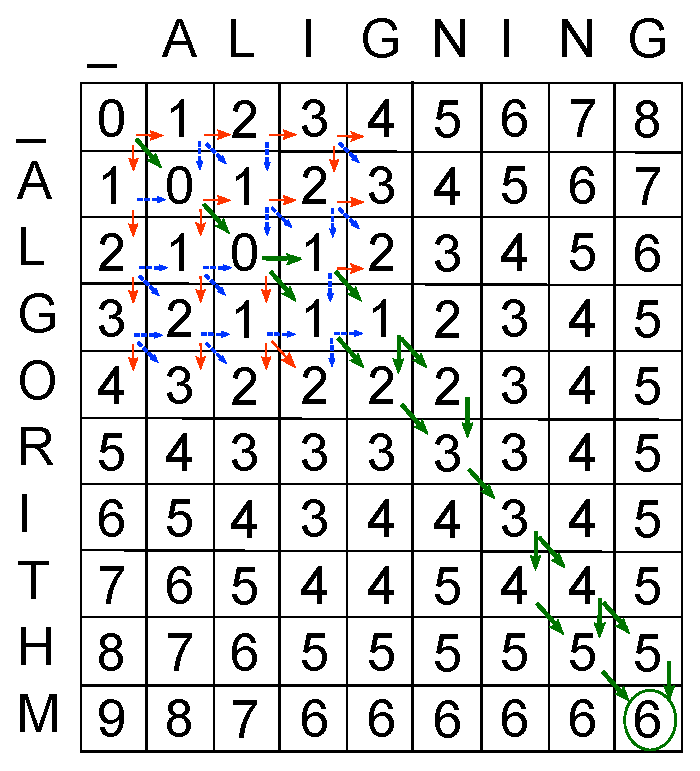
\includegraphics[scale=0.6]{img-align/edit-distance.eps}
	\caption[Edit Distance alignment] {Edit Distance matrix for sequences 'algorithm' and 'aligning', using unitary costs. The first dependencies are marked. The non-picked directions have dotted blue lines, picked ones are red and straight, and the optimal path is in green bold.}
	\label{edit-distance}
  \end{minipage}
  \hspace{0.04\linewidth}
  \begin{minipage}{0.48\linewidth}
	\centering
	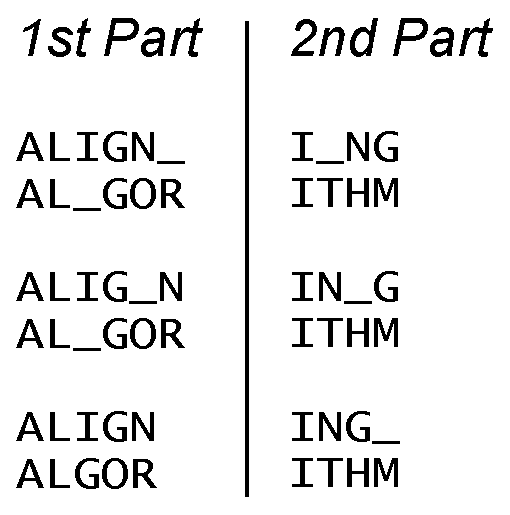
\includegraphics[scale=0.5]{img-align/alignments.eps}
	\caption[Resulting optimal alignments from Edit Distance]{Resulting 9 optimal alignments - each part from the left concatenated with a right part. All the alignments have the last I's aligned, and there are 3 possible variations before and after the I's.}
	\label{alignments}
  \end{minipage}
\end{figure} 

%\begin{figure}[h]   % h, here.  t, top.  b, bottom.  p, page of float
%	\centering
%	\subfigure[Edit Distance matrix for sequences 'algorithm' and 'aligning', using unitary costs. The first dependencies are marked. The chosen directions are in red, the optimal path in green.] {
%		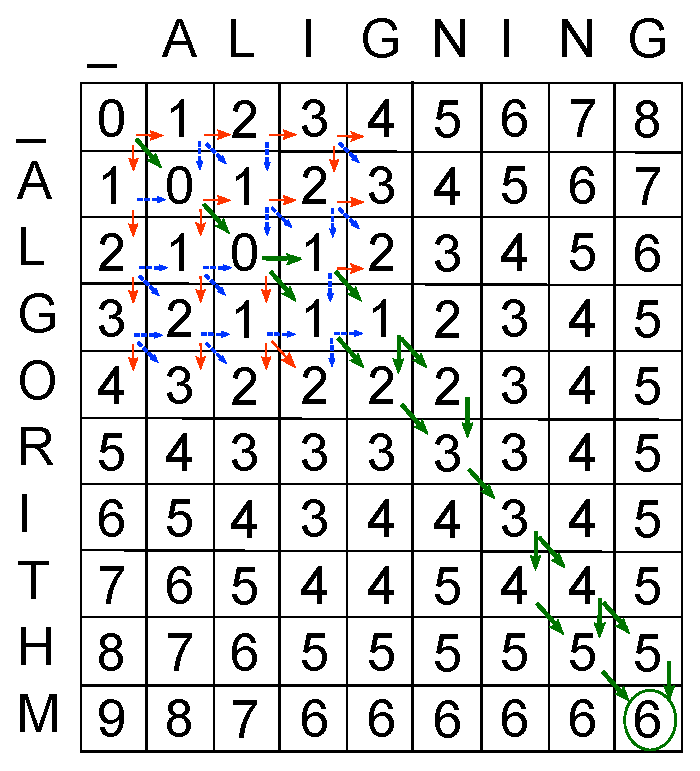
\includegraphics[scale=0.5] {img-align/edit-distance.eps}
%		\label{edit-distance}
%	}
%	\hspace*{0.5cm}
%	\subfigure[Resulting 9 optimal alignments - each part from the left concatenated with a right part. All the alignments have the last I's aligned, and there are 3 possible variations before and after the I's.] {
%		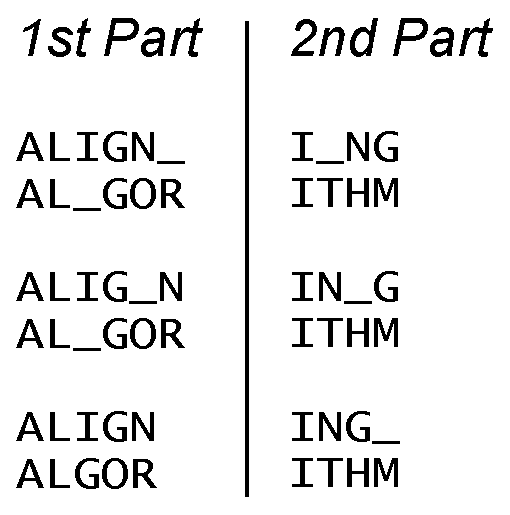
\includegraphics[scale=0.5] {img-align/alignments.eps}
%		\label{alignments}
%	}
%	%\caption{A figure example.}
%	%\label{fig:rmain figure}
%\end{figure}




%Edit distance of Damerau
%There is however a main limitation of Levenshtein's metric - it does not consider as a single 'edit operation' the transposition of elements. To face this problem, Damerau in 1964 \cite{damerau} proposed a new metric, with the 3 edit operations of Levenshtein and a new 4th operation - switching of two consecutive symbols. This is a very common source of misspellings, which was Damerau's motivation for the introduction of the new distance metric. The Levenshtein metric with Damerau's improvement is known as Levenshtein-Damerau Distance.




%%%%%%%%%%%%%%%%%%%%%%%%%%%%%%%%%%%%%%%%%%%%%%%%%%%%%%%%%%%%%%%%%%%%%%%
%%%%%%%%%%%%%%%%%%%%%%%%%%%%%%%%%%%%%%%%%%%%%%%%%%%%%%%%%%%%%%%%%%%%%%%

\subsection{\ac{NW} Algorithm for Global Alignment}

In 1970 \cite{needlemanwunsch} Needleman and Wunsch adapted the Levenshtein metric to use in the field of biological alignment. The \ac{NW} algorithm is mostly similar to the later Wagner and Fischer algorithm, with two differences introduced to improve its biological meaning:

	- Gaps are considered a single mutational event. A single "gap opening" penalty is weighted each time the alignment may evolve from a continuous region to a gap;

	- Each substitution may have a different real-world occurrence probability, and hence it should have a different weight. These probabilities were later measured and tabulated (see \sref{Substitution Scoring matrices}).

The resulting score of a global alignment, like that of a levenshtein edit distance, is given by the score of the last cell (which is the score of the complete path between the start of both sequences and their end). The function used for each cell may be the maximum or the minimum of previous cells.

Needleman and Wunsch's original metric for single gaps, and Sellers' similar method \cite{smith1981comparative}, were later extended by Waterman in 1976 \cite{waterman1976some} to support an arbitrary number of deletions/insertions and more complex gap cost models. Since then, all global alignment metrics and algorithms based on edit distances used for biological alignment are referred to as Needleman-Wunsch's.

Any type of function can be used for gap scoring, tough the function used has a great impact on the algorithm's complexity. If a linear cost function is used, each cell's value can be computed by inspecting only its direct ascendants (horizontal, vertical and diagonal). However, when using a non-linear cost function, such as an affine function with an initial gap opening constant penalty, this is not the case. Given the complex behavior of these functions, each value cannot be completely inferred from the previous discrete value. The contribution of a gap sequence may 'skip' some cells (usually the first) because the diagonal value presents a better option; and still be chosen for later cells, due to the function's amortized behavior (see \autoref{nw-complex-cost-models}). This means that, in order to compute each cell, the contributions of all the previous cells have to be considered and computed, and hence the algorithm's complexity rises from $O(n \times  m)$ to $O(n \times m \times max(n,m))$. 

\begin{figure}[htb!]
\centering
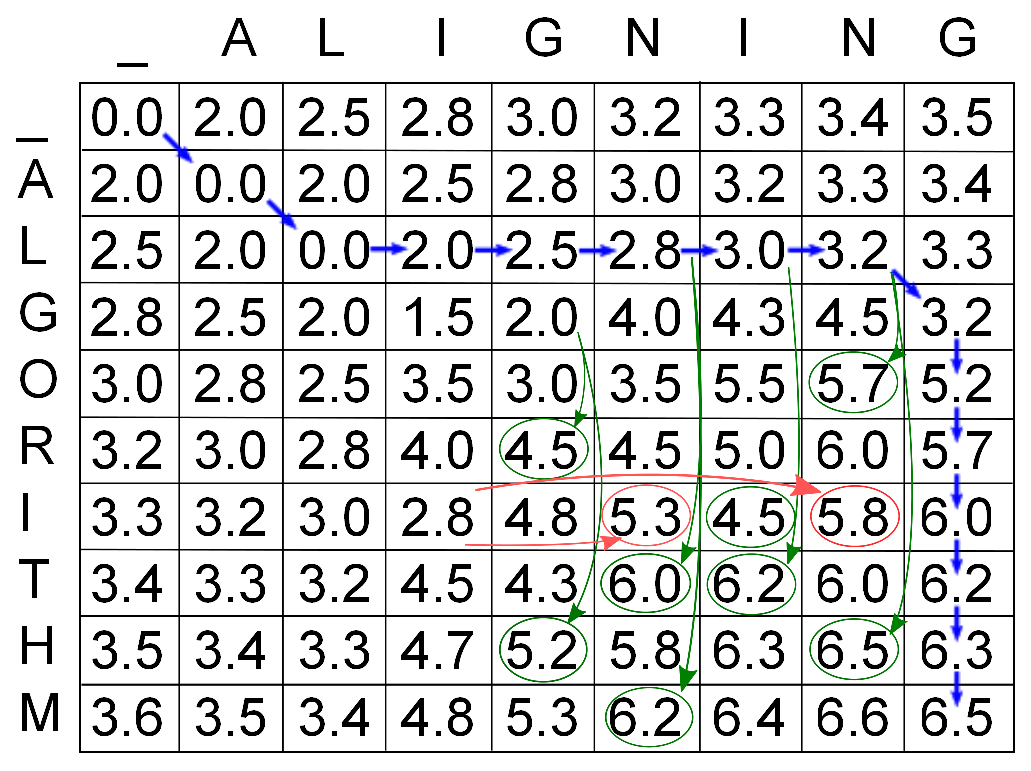
\includegraphics[scale=0.6]{img-align/nw-complex-cost-models.eps}
\caption[Needleman-Wunsch alignment] {Needleman-Wunsch matrix with a logarithmic gap model ($GapCost = 2 + 0.5 \times log_2(\#gaps)$, Match 0, Mismatch 1.5). Red and green arrows show the chosen non-continuous gaps (i.e. that are only chosen in later cells). The optimal alignment is traced in blue bold lines.}
\label{nw-complex-cost-models}
\end{figure}



\subsection{\ac{SW} Algorithm for Local Alignment}
\label{Smith-Waterman algorithm for Local Alignment}

Despite the good results of the \ac{NW} algorithm, most of the time molecular biologists do not want a global alignment. A global alignment forces all the sequences to be aligned - one way or the other. This means that, if there are regions with high similarity and regions with high divergence, the overall result would be average, or even bad. The interesting regions cannot be identified and extracted from the complete alignment. Moreover, global alignments always force the inclusion of gaps on the alignment fringes.

To tackle these limitations of global alignment, Smith and Waterman in 1981 \cite{smithwaterman} extended the previous algorithms with the possibility of "alignment restart", thus creating the first algorithm to compute local alignments (in \autoref{smith-waterman}). The \ac{SW} algorithm is similar to \ac{NW}'s and Sellers', with the differences:

	- Each cell value is maximized with 0. This mechanism causes a 'restarting' in the alignment path. Naturally, this requires the penalties to be negative and the match scores positive.

	- The maximum score may be obtained from any cell of of the matrix, instead of only the last one. Each cell holds the score for the optimal local alignment that ends in that cell.

	- To compute the gap cost, only those previous cells before the first zero (when followed backwards from the current cell) need to be inspected. All more distant previous cells cannot lead to a positive gap score.

\begin{figure}[htb!]
\centering
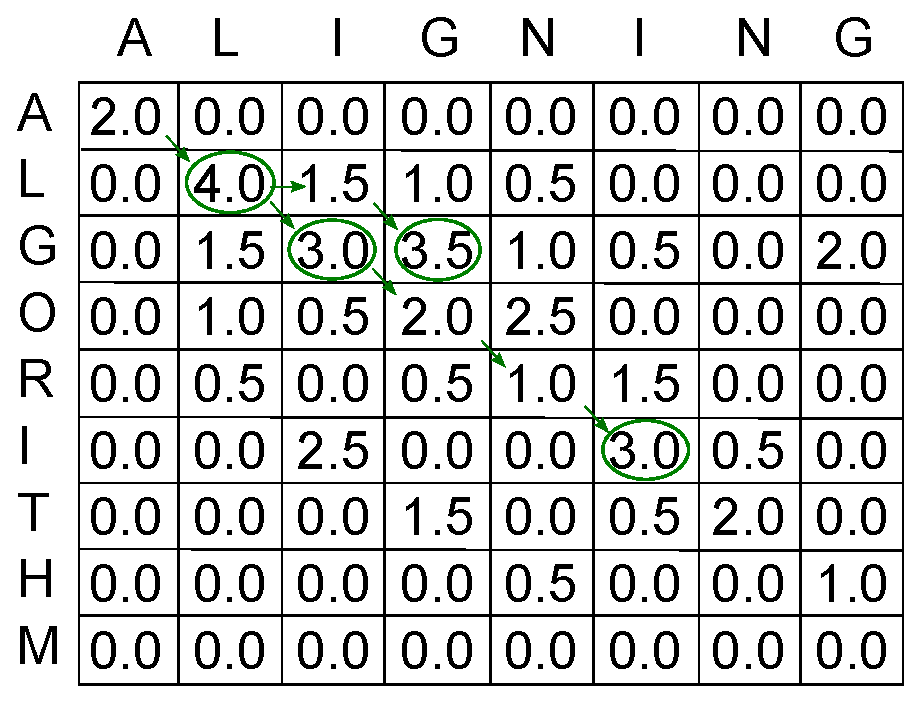
\includegraphics[scale=0.5]{img-align/smith-waterman.eps}
\caption[Smith-Waterman alignment] {Smith-waterman algorithm. $GapCost = -2 -0.5 \times (\#gaps)$, Match +2, Mismatch -1. The best alignments are shown and traced, with the maximum values circled.}
\label{smith-waterman}
\end{figure}


\subsection{Gotoh Algorithm}
\label{Gotoh algorithm}

These \ac{DP} algorithms are overly simple, and only a few optimizations have been found to reduce the required time and space lower bound. The quadratic time barrier cannot be lowered since they require that every cell in the $N \times M$ be computed. For arbitrary cost models, the complexity is even worse ($O(n^3)$). However, for some restricted cost models, a few improvements are possible.

Gotoh in 1982 \cite{gotoh} proposed a very important optimization for general \ac{DP} algorithms that use affine scoring functions. Such functions are actually one of the most suitable to biological sequences. Each gap opening is highly penalized, and all successive gaps have a reduced, linear cost, which models quite well the real-world occurrence of single mutational events, frequently responsible for inserting/deleting many elements at once.

Gotoh's algorithm is based upon the idea that the gap costs can also be modeled and computed in parallel, using Dynamic Programming, in separate matrices for vertical and horizontal gaps. Each cell in these two matrices hold the cost for a gap that ends in that cell.

These two matrices are computed based on their own dependencies and on the respective value in the main distance matrix (choosing the current main score 'restarts' the gap sequence, opening a new gap from the current cell). For the main matrix, the match/mismatch value is taken from its previous diagonal cell, and the gap contributions come from the same cell in the two twin matrices (i.e. the cost of a horizontal or vertical gap ending in that cell).

The gap matrices are usually named Q and P (after Gotoh), or E (horizontal) and F (vertical), while the main matrix is called D (distance matrix). The recursion relation can be formulated as follows:
\hspace{2 pc}  $$D_{m,n} = OP ( D_{m-1,n-1} + d(a_m,b_n) , E_{m,n} , F_{m,n} ) $$
Where OP may be Maximum or Minimum, and $d(a_m,b_n)$ is the match/mismatch score for the pair of elements $(a_m,b_n)$. E and F are both given by the same identical relation:
\hspace{2 pc}  $$E{m,n} = OP ( D_{m-1,n} + W_1 , E_{m-1,n} + W_{ext} ) 
\hspace{2 pc}  F{m,n} = OP ( D_{m,n-1} + W_1 , F_{m,n-1} + W_{ext} ) $$
$W_1$ is the gap cost function value for one gap, and $W_{ext}$ is the gap extension penalty, which is the slope of the affine cost function W. $W_i = W_{open} + i \times W_{ext}$. An example is presented in the associated figures.

Besides the reduced number of previous values that need be seen to compute each cell, Gotoh's improvement has another precious effect: the whole matrices are themselves not needed. They have to be computed but do not need to be stored, since only the last line column of diagonal of each one is used. As such, the algorithm can be very efficiently implemented on a computer, using only three of two arrays to store the intermediate cells. Gotoh's algorithm, therefore, reduces the time complexity to $O(N \times M)$ and the space complexity to O(min(n,m)).

One important note though, about reduced space requirements: gotoh's algorithm computes only the optimal score (or a set of scores, if they are saved separately). The alignment pattern itself cannot be extracted when this method is used, since no tracebacking data is stored.

\begin{figure}[htb!]
  \begin{minipage}{0.26\linewidth}
	\centering
	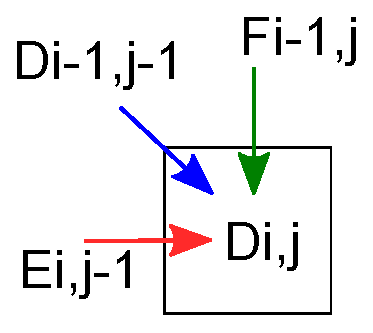
\includegraphics[scale=0.5]{img-align/nw-affine-gotoh-deps.eps}
	\caption[Gotoh's dependencies] {Dependencies for each cell of Gotoh's algorithm. Diagonal, horizontal and vertical.}
	\label{nw-affine-gotoh-deps}
  \end{minipage}
  \hspace{0.04\linewidth}
  \begin{minipage}{0.7\linewidth}
	\centering
	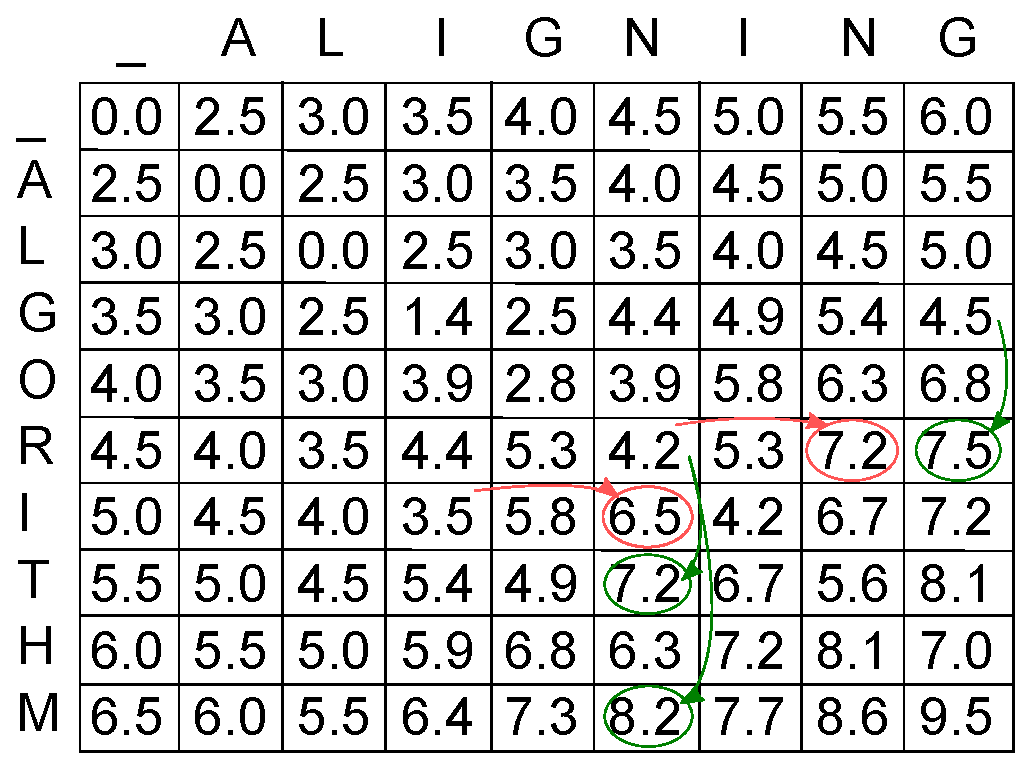
\includegraphics[scale=0.5]{img-align/nw-affine-gotoh-Dmat.eps}
	\caption[Gotoh's main matrix] {Gotoh's \ac{NW} algorithm D main matrix, with $GapCost = 2+0.5 \times (\#gaps)$, Match 0, Mismatch 1.4. Rightwards values in red come from the E matrix, and downwards green values from the F matrix.}
	\label{nw-affine-gotoh-Dmat}
  \end{minipage}
\end{figure} 


\begin{figure}[htb!]
 \begin{minipage}{0.48\linewidth}
	\centering
	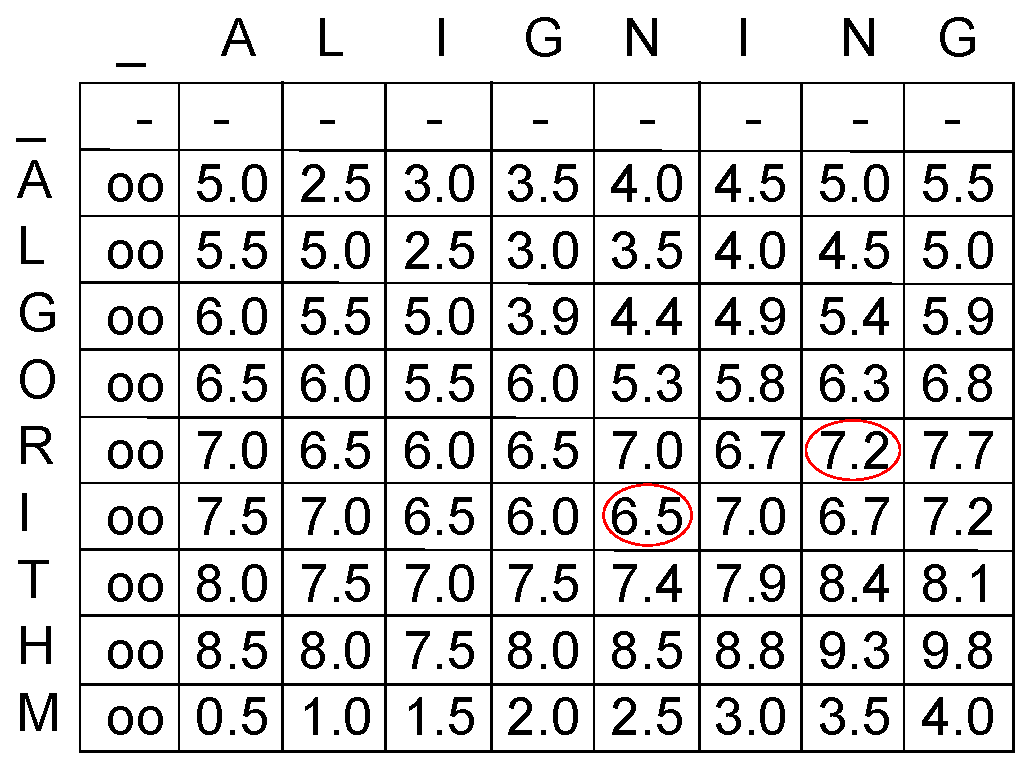
\includegraphics[scale=0.45]{img-align/nw-affine-gotoh-Emat.eps}
	\caption[Gotoh's E matrix] {Gotoh's left gaps (E) matrix. The values chosen for the main matrix are marked.}
	\label{nw-affine-gotoh-Emat}
  \end{minipage}
  \hspace{0.04\linewidth}
  \begin{minipage}{0.48\linewidth}
	\centering
	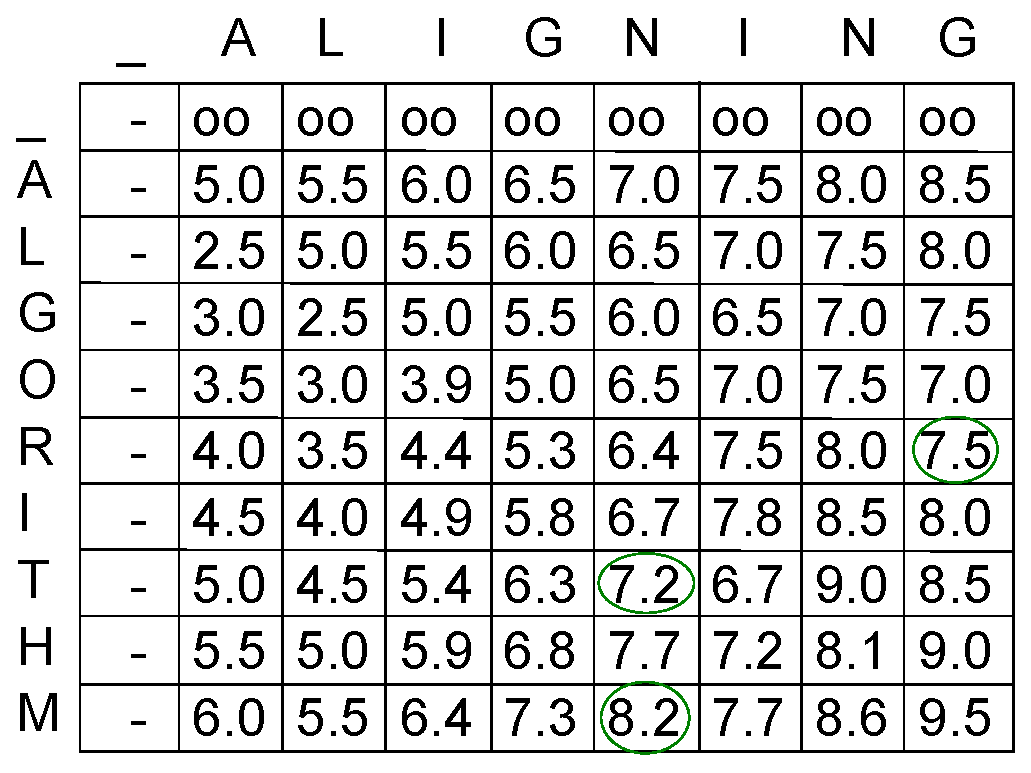
\includegraphics[scale=0.45]{img-align/nw-affine-gotoh-Fmat.eps}
	\caption[Gotoh's F matrix] {Gotoh's vertical gaps (F) matrix. The values chosen for the main matrix are marked.}
	\label{nw-affine-gotoh-Fmat}
  \end{minipage}
\end{figure} 



\subsection{SWAT optimization of the Smith-Waterman Algorithm}
\label{SWAT optimization}

%This improvement of the \ac{SW} algorithm is named after Green which first used it to great success in his 1993's SWAT program \cite{swat}. Pearson in 1991 had already implemented a similar optimization in the alignment kernel of FASTA, ssearch \cite{ssearch}.

For most sequences and typical scores, the D value in the Smith-Waterman algorithm remains at 0, or close by, in the majority of matrix cells (see \autoref{smith-waterman}). The E (horizontal) and F (vertical) dependencies can only affect D when the D value is higher (i.e. worse) than the weight of a single gap ($W_1 = W_{open} + 1 \times W_{ext}$). Such a penalty is usually chosen to be considerable costly, sometimes double the cost of a mismatch. Owing to that, only in relatively few cells are the E and F vectors able to affect the D cell value.

The SWAT optimization (\cite{swat},\cite{ssearch}) exploits this tendency. It consists of a relaxation in the required cells that need to be seen to evaluate the gap dependencies: all F and E cells lower than $W_1$ cannot contribute to the alignment, and neither can all cells before those, because they would offer a worse gap starting point. Therefore the previously presented zero-barrier may be extended to a $W_1$-barrier.

Using the original zero-barrier and this optimization, the cubic complexity of the \ac{SW} algorithm can be lowered in practice to $O(a \times n \times m)$, where '$a$' is some empirical constant. The Gotoh variant can also be greatly improved with these barriers, by ignoring the E and F values below the threshold.


%%%%%%%%%%%%%%%%%%%%%%%%%%%%%%%%%%%%%%%%%%%%%%%%%%%%%%%%%%%%%%%%%%%%%%%
%%%%%%%%%%%%%%%%%%%%%%%%%%%%%%%%%%%%%%%%%%%%%%%%%%%%%%%%%%%%%%%%%%%%%%%

\subsection{Substitution Scoring matrices}
\label{Substitution Scoring matrices}

Alignment algorithms operate on the special context of biological systems. Each sequence base (or residue) has a specific and distinct nature. Some are more frequent than others, some degenerate and mutate more easily, some are found more frequently in some regions. In particular, each symbol has a different probability of mutation into each other specific symbol. In order to accurately study and predict these dynamic biological events, the scoring system used to evaluate each sequence pair must take all this into account, and it must be constructed and trained with real biological data (i.e. mutations empirically observed in proteins and nucleic acids). These values were measured by Dayhoff in 1978 \cite{pam} to create PAM matrices, and by Henikoff in 1992 \cite{blosum} in the form of BLOSUM matrices, using a logarithmic scale. The two matrix types use opposite scoring schemes: PAMs were constructed from the observed mutations along a phylogenetic tree, whereas BLOSUMs measure the conserved regions. A lower PAM (fewer mutations) corresponds to a higher BLOSUM (more conservation), and vice versa.

An extension of the concept of substitution scores matrix is the \acp{PSSM}, also known as (Position Specific) Weight matrices, Frequency matrices or Profile matrices. These matrices count the number of occurrences of each symbol (line), for each sequence position (row). Employing \acp{PSSM} instead of simple substitution matrices has been proven to better model the sequences' homology. \cite{gribskov1987profile} \cite{henikoff1994position} \cite{rudnickipssms}



%%%%%%%%%%%%%%%%%%%%%%%%%%%%%%%%%%%%%%%%%%%%%%%%%%%%%%%%%%%%%%%%%%%%%%%
%%%%%%%%%%%%%%%%%%%%%%%%%%%%%%%%%%%%%%%%%%%%%%%%%%%%%%%%%%%%%%%%%%%%%%%
%%%%%%%%%%%%%%%%%%%%%%%%%%%%%%%%%%%%%%%%%%%%%%%%%%%%%%%%%%%%%%%%%%%%%%%
%%%%%%%%%%%%%%%%%%%%%%%%%%%%%%%%%%%%%%%%%%%%%%%%%%%%%%%%%%%%%%%%%%%%%%%







%%%%%%%%%%%%%%%%%%%%%%%%%%%%%%%%%%%%%%%%%%%%%%%%%%%%%%%%%%%%%%%%%%%%%%%%%%%%%%%%%%%%%%%%%%%%%%%%%%%%%%%
%%%%%%%%%%%%%%%%%%%%%%%%%%%%%%%%%%%%%%%%%%%%%%%%%%%%%%%%%%%%%%%%%%%%%%%%%%%%%%%%%%%%%%%%%%%%%%%%%%%%%%%
%%%%%%%%%%%%%%%%%%%%%%%%%%%%%%%%%%%%%%%%%%%%%%%%%%%%%%%%%%%%%%%%%%%%%%%%%%%%%%%%%%%%%%%%%%%%%%%%%%%%%%%
%%%%%%%%%%%%%%%%%%%%%%%%%%%%%%%%%%%%%%%%%%%%%%%%%%%%%%%%%%%%%%%%%%%%%%%%%%%%%%%%%%%%%%%%%%%%%%%%%%%%%%%

\section{Homology Search with Markov Models}

In this section, a different approach to sequence homology search will be described, an approach based on Hidden Markov Models. Despite the differen formulation of the problem, the  computation involved is very similar, and thus the algorithms and parallelization methods previusly analyzed, for the most part, can equally be used with Markov Models. 


\subsection{Markov Models}

In this section,  we will first introduce very briefly what are Markov Models.
A Markov Model is a probabilistic model of a system which enjoys the Markov property: the future states of the system depend entirely on the present state, and not on any previous states. A Hidden Markov Model (abbreviated HMM) is a Markov Model with unobserved states, so called 'hidden states'. In a HMM, the states may emit more than one possible token, according to a probability distribution. A HMM is therefore characterized by a number of unobserved states Q; a number of possible emission tokens T; a probability distribution of transitioning between the states Ft(q1,q2); and a probability distribution of emitting each token in each state Fe(q,w). The probability of some specific sequence of tokens being generated by a specific path of states $\pi$ is then given by:
$$P(x,\pi) = t_{0\pi_1} \prod\nolimits_{i=1}^L e_{\pi_i}(x_i) \times t_{\pi_i \pi_{i+1} }  $$

When using HMM, there are two tasks that are particularly important:
\begin{itemize}
	
	\item Decoding: Which path of states is the more likely to have generated a given token sequence, and what is the corresponding probability?
	This task is computed by the Viterbi Algorithm \cite{viterbi}, which progressively computes the most likely state to generate each new output symbol (i.e. token) , from the begin pseudo-state until reaching the end pseudo-state.	
	For each sucessive sequence symbol $x_i$, the Viterbi algorithm computes the recursive relations:
	$$ V_l(i) = e_l(x_i) \times max_k ( V_k (i-1) \times t_{kl} ) $$
	$$ Ptr_i(l) = argmax_k (V_k (i-1) \times t_{kl} ) $$	
	with $V_l(i)$ being the probability of being in state $l$, and emitting symbol $x_i$, and $Ptr_i(l)$ being the pointer to the chosen previous state.	
	To recover the most likely path, one must only traverse the computed pointers, $Ptr_i(l)$, in the reverse direction, from the end-state to begin-state.	
	
	\item Generation: What is the likelihood of a given sequence being generated by the model?

	To compute the likelihood probability, we need to sum the probabilities of all the possible generation paths. Since the number of possible paths is exponential, a more efficient method must be used. A solution is given by the Forward algorithm, which is similar to the Viterbi algorithm: a progressive sum of the probabilities of all previous state paths for each new token.

	For each sucessive sequence symbol $x_i$, the Forward procedure computes the following relation:
	$$ F_l(i) = e_l(x_i) \sum\limits_k F_k (i-1) \times t_{kl}  $$
	The final probability is calculated by summing the final probabilities of all the states:
	$$ F(x) = \sum\limits_k F_k (L) \times t_{k0}  $$
\end{itemize}

These two procedures can encounter value representation problems when implemented on a computer. Since they involve sucessive products of small probabilities, especially the Viterbi algorithm, the computed probalities quickly exceed the floating-point representation range of modern computers and go into underflow. This can be avoided by working in log-space, with logarithmic probabilities in every calculation, and the products turned into sums.

\label{log-transform}
The Logarithmic transformation poses a problem in the Forward algorithm: the log of a sum of two arguments is not easily computed from the logs of the arguments. The exact value is given by  $ \tilde{r} = log (exp(\tilde{a_1}) + exp(\tilde{a_2})) $, which can be written as $ \tilde{ r } = \tilde{a_1} + log (1 + exp(\tilde{a_2} - \tilde{a_1}))$. However, the function $log (1 + exp(\tilde{a_2} - \tilde{a_1}))$ can be approximated by interpolation from a table with a reasonably small size. \cite{hmmsbook}.

HMM have been used quite successfully for the past decades for various applications of statistical modeling and machine learning \cite{hmms-speech}.




\subsection{Alignment Profiles}

Until now, we have been looking at the homology search problem through the process of single alignment of one sequence against another.
In real applications however, namely for searching homologs (i.e. similar sequences) in a databse, we are looking for sequences that belong to a certain family or have a high similarity to a given group of sequences. Therefore, it is oftentimes more useful to search and compare the database against a group of sequences instead of a single query.

%\begin{figure}[htb!]
%  \begin{center}
%    \resizebox*{0.5\columnwidth}{!}{ 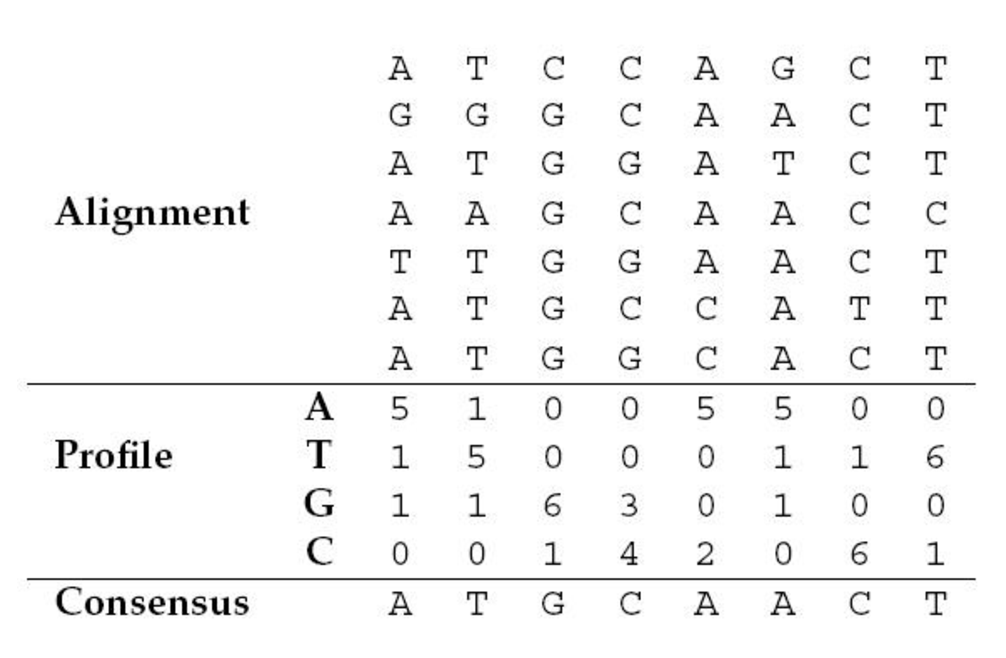
\includegraphics{img-align/consensus-profile.eps} }
%    \caption[Consensus Profile] {Example of a Consensus Profile derived from a multiple alignment of a family of similar sequences.}
%    \label{consensus-profile}
%  \end{center}
%\end{figure}

\begin{table}[h!]
\centering
\caption[Consensus Profile example] {Example of a Consensus Profile derived from a multiple alignment of a family of similar sequences.}
\label{consensus-profile}

\begin{tabular}{cccccccccc}
\multirow{6}{*}{\textbf{Alignment}} &  & A & T & C & C & A & G & C & T \\
&  & G & G & G & C & A & A & C & T \\
&  & A & T & G & G & A & T & C & T \\
&  & A & A & G & C & A & A & C & C \\
&  & A & T & G & C & C & A & T & T \\
&  & A & T & G & G & C & A & C & T \\
\hline
\multirow{4}{*}{\textbf{Profile }} & \textbf{A} & 5 & 1 & 0 & 0 & 5 & 5 & 0 & 0 \\
& \textbf{C} & 0 & 0 & 1 & 4 & 2 & 0 & 6 & 1 \\
& \textbf{G} & 1 & 1 & 6 & 3 & 0 & 1 & 0 & 0 \\
& \textbf{T} & 1 & 5 & 0 & 0 & 0 & 1 & 1 & 6 \\
\hline
\textbf{Consensus} &  & A & T & G & C & A & A & C & T \\
\end{tabular}
\end{table}

Profiles provide a more flexible way to identify homologs of a certain family, by highlighting the family's common features, and downplaying the divergences between the family's sequences. There are many ways to generate profiles, but most involve an initial multiple alignment of the sequences, followed by a probabilistic breakdown of the elements (residues or base-pairs) present in each position.

Profiles can thus effectively model a whole sequence family. This allows for a more efficient homology search: instead of comparing a query to each sequence in the family, the query can be compared to the Profile alone, greatly reducing the involved computational cost. Besides, a Profile gives a more correct representation of the defining characteristics of a family, by weighing the elements in proportion to their actual frequency (and thus importance) in the underlying family.



\subsection{Profile Markov Models}

A promising and widely used type of Profile constructs are Hidden Markov Models \cite{hmms}. 

Hidden Markov Models can be used to statistically model the distribution of sequence elements in a Profile, capturing the probability of each element in each position as the emission probability of tokens in each state. In such a model, each model state represents one position of the family consensus.
These Profile HMMs are then used to search a sequence database, by computing the probability of each database sequence being generated by the query model.

HMMs may also be used to find distant homologs by iteratively building and refining a model that describes them (such as in the SAM tool, \cite{sam}). In such an application, we start with an empty model. Iteratively,  each new sequence is aligned against the model, and that alignment is used to add the sequence to the multiple alignment of sequences that underlie the model. Finally the model is re-parametrized with the new multiple alignment.

Krogh and Haussler in 1994 \cite{krogh1994} developed a straightforward generalized profile Hidden Markov Model for homology searches, that emulate the results of a optimal alignment algorithm. The model is composed by three different types of states, respectively for matches/mismatches, insertions and deletions.

\begin{figure}[htb!]
	\begin{minipage}{0.48\linewidth}
		\centering
		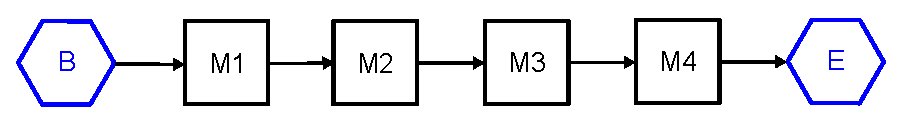
\includegraphics[scale=0.5]{img-hmm/model-construction-matches.eps}
		\caption[HMM for ungapped global alignment] {Example of a HMM composed solely of match states, allowing for ungapped global alignment.}
		\label{model-construction-matches}
	\end{minipage}
	\hspace{0.04\linewidth}
	\begin{minipage}{0.48\linewidth}
		\centering
		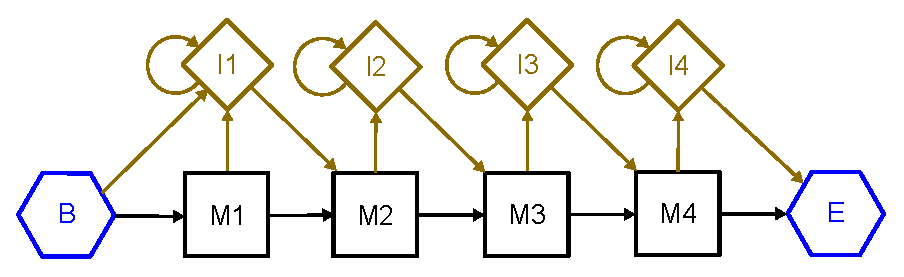
\includegraphics[scale=0.5]{img-hmm/model-construction-inserts.eps}
		\caption[HMM with Insert gaps] {Example of a HMM that allows arbitrary insertions. }
		\label{model-construction-inserts}
	\end{minipage}
\end{figure} 

The construction of the model is intuitive. First, a simple ungapped global alignment is modeled by a succession of match states, with a single string of transitions, as seen in \autoref{model-construction-matches}. These match states emit the alignment symbols, so they have a corresponding emission probability distribution, which is derived from the relative frequencies of symbols in the family's sequences. Since the symbols' frequencies vary in each position of the family's Profile, the emission distribution of the model, $e_{M_i}(x)$, will also be position-specific (similar to a \ac{PSSM}, see \sref{Substitution Scoring matrices}).

Our objective is to determine if a given sequence belongs to the model's family, so we have to discriminate the positive probability (sequence X generated by that model) against the negative probability (sequence X generated by some other random model). The negative probability is the background probability distribution, ${q_x}$., i.e., the probability of belonging to the standard random model. This is evaluated for the emission probabilities, in the form of log-odds ratios:

$ S(x) = log \frac{P(x|model)} {P(x|random)} = \sum\limits_{i=-1}^L log \frac{e_i{x_i}} {q_{x_i}} $

After having a model of match states for ungapped global alignment, we proceed to deal with gaps. It is possible to handle insertions (i.e., sections of the sequence $x$ that do not match the model) with an extra layer of states - insert states. An inserted region can occur at any point in the model, so we need to include an Insert state between each pair of match states. These new insert states must have a loop to allow for arbitrarily long inserted regions. A sketch of the resulting model with match and insert states is shown in \autoref{model-construction-inserts}.

These insert states also have an emission probability distribution $e_{I_i}(x)$, that represents the inserted symbols. This distribution however is arbitrary, it does not depend on the model, since these inserted elements are unknown to the model. To simplify the calculations, the insert emissions $e_{I_i}(x)$ are usually set to the background distribution ${q_x}$, resulting in a null odds-ratio contribution. The I $\rightarrow$ I model the gap-extend costs for non-matched symbols in the query sequence.

Lastly, deletions (portions of the profile not matched by the sequence) are added to the model, as forward jumps from each match state to every other suceeding match state. Each of the $N$ match states will have one average $\frac{N}{2}$ forward transitions. The basic idea is shown in \autoref{hmm-jumps1}. However, a topology with these forward jumps faces a cumbersome problem: the number of added transitions, $\frac{N^2}{2})$, is quite large, and can significantly slow down any algorithm. 

To circumvent the $\frac{N^2}{2})$ transitions, it is possible to develop an alternative topology that makes use of a third sucessive layer of silent 'jump states'. Silent states are those that do not emit any output symbol, but they may serve an important purpose in simplyfing a model. A forward jump is then achieved by sucessive transitions along the 'jump states' from one match state to the other, instead of a single transition between the two match states. A topology with jump states has the major advantage of using only a linear number of transitions ($N\times2$ new transitions) and new states ($N$ new states). An example of this topology is shown in \autoref{hmm-jumps2}.

\begin{figure}[htb!]
	\begin{minipage}{0.48\linewidth}
		\centering
		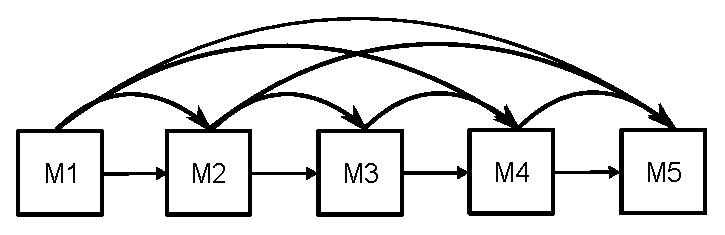
\includegraphics[scale=0.6]{img-hmm/hmm-jumps1.eps}
		\caption[HMM with Delete gaps] {Example of a HMM with a continuous sequence of states, and arbitrary jumps ahead.}
		\label{hmm-jumps1}
	\end{minipage}
	\hspace{0.04\linewidth}
	\begin{minipage}{0.48\linewidth}
		\centering
		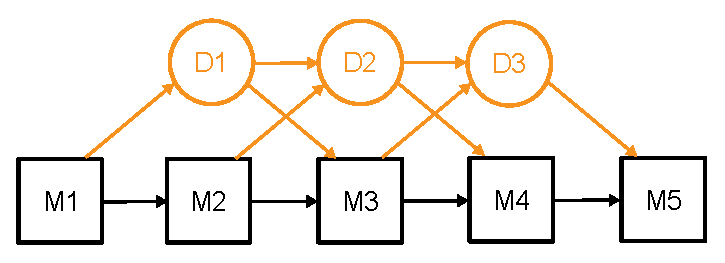
\includegraphics[scale=0.6]{img-hmm/hmm-jumps2.eps}
		\caption[HMM with Jump states] {Example of the previous HMM with the forward jump transitions converted to a layer of silent 'jump states'.}
		\label{hmm-jumps2}
	\end{minipage}
\end{figure} 

We can therefore use the 'jump states' as Delete states, where in each forward jump represents a region deleted from the profile model in the alignment. The D $\rightarrow$ D transitions thus correspond to gap-extend costs. Finally, the new layer of Delete states is added our previous model, which only had two layers, namely matches and inserts. Additional transitions from insert states to delete states, and vice-versa, can be included for the sake of correctness, although these transitions are usually very improbable and have a negligible effect. The final model for gapped global alignment, as proposed by Krogh and Haussler \cite{krogh1994}, can be seen in \autoref{krogh-haussler-model}. Krogh-Haussler's model is quite simple and intuitive, and has become the blueprint for later Profile HMMs \cite{sam}.

After having decided the structure of the HMM, it is necessary to parametrize it with the given family of sequences, namely to calculate from the data all the probability distributions required for the HMM. The parameterization of HMMs is a complex subject that falls outside the scope of this work (for this subject, see \cite{hmmsbook}). The Viterbi algorithm is also used for this purpose.

% STRESSAR que nao vamos abordar as formas de parametrizacao e os parametros usados no HMM
% Colunas com mais gaps que elementos sao modeladas por inserts

\begin{figure}[htb!]
  \begin{center}
    \resizebox*{1.0\columnwidth}{!}{ 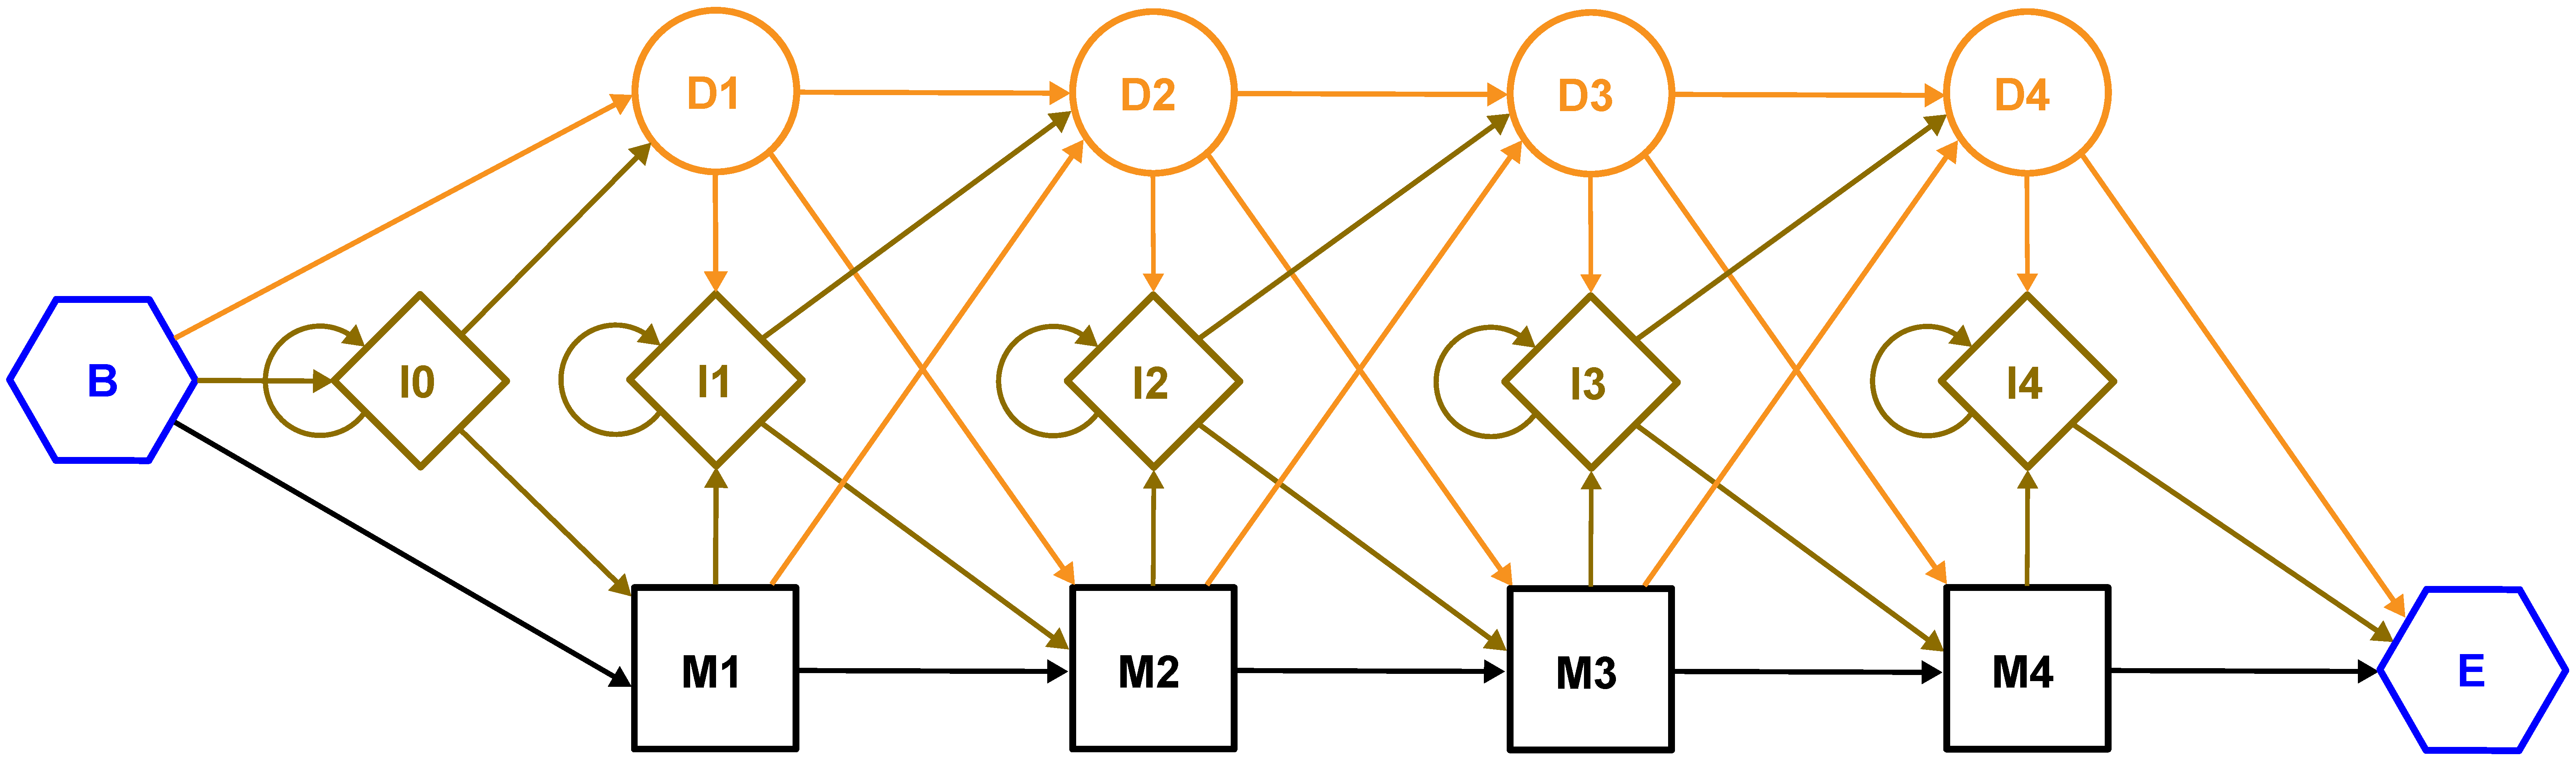
\includegraphics{img-hmm/krogh-haussler-model.eps} }
    \caption[HMM of Krogh-Haussler] {Krogh and Haussler' Hidden Markov Model for optimal gapped global alignment.}
    \label{krogh-haussler-model}
  \end{center}
\end{figure}





\subsection{Algorithms for global alignment Profile HMMs}

In a Profile HMM, the Viterbi algorithm gives the most likely path of states to generate the sequence, and the corresponding probability. It is therefore suitable for computing the alignment of the query sequence against the already multiple-aligned family's sequences (represented by the HMM). 

The Forward algorithm computes the overall likelihood of the sequence being generated by that model through any path, as opposed to a random model, by summing the probabilities of all possible paths. It is thus more suitable as a general similarity measure, indicating the likelihood of the query sequence belonging to the family.

For a global alignment Krogh-Haussler model, working in log-space, the Viterbi algorithm is expressed by the following \ac{DP} recurrence relations:
$$ V^M_j(i) = log \frac{e_{Mj}(x_i) }{q_{xi}} + Max  
		\begin{cases}
			V^M_{j-1} (i-1) + log\ t_{M_{j-1} M_j}  \\
			V^I_{j-1} (i-1) + log\ t_{I_{j-1} M_j}  \\
			V^D_{j-1} (i-1) + log\ t_{D_{j-1} M_j} 
		\end{cases} $$

$$ V^I_j(i) = log \frac{e_{Ij}(x_i) }{q_{xi}} + Max  
		\begin{cases}
			V^M_{j} (i-1) + log\ t_{M_{j} I_j}  \\
			V^I_{j} (i-1) + log\ t_{I_{j} I_j}  \\
			V^D_{j} (i-1) + log\ t_{D_{j} I_j}
		\end{cases} $$
$$V^D_j(i) = Max \begin{cases}
			V^M_{j-1} (i) + log\ t_{M_{j-1} D_j}  \\
			V^I_{j-1} (i) + log\ t_{I_{j-1} D_j}  \\
			V^D_{j-1} (i) + log\ t_{D_{j-1} D_j} 
		\end{cases} $$
$$ \\ $$

In regards to the Forward algorithms, for a global alignment model, working in log-space, we need to deal with following equations:
\begin{align*}
 F^M_j(i) = log \frac{e_{Mj}(x_i) }{q_{xi}} + log \;\;  
		[ \;\;  &t_{M_{j-1} M_j} \times exp \; (F^M_{j-1}(i-1))  \\ 
		+\;\;  &t_{I_{j-1} M_j}  \times exp \; (F^I_{j-1}(i-1))  \\
		+\;\;  &t_{D_{j-1} M_j} \times exp \; (F^D_{j-1}(i-1)) \;\; ] 
\end{align*}
\begin{align*}
 F^I_j(i) = log \frac{e_{Ij}(x_i) }{q_{xi}} + log \;\;  
		[ \;\;  &t_{M_{j} I_j} \times exp \; (F^M_{j}(i-1))  \\ 
		+\;\;  &t_{I_{j} I_j}  \times exp \; (F^I_{j}(i-1))  \\
		+\;\;  &t_{D_{j} I_j} \times exp \; (F^D_{j}(i-1)) \;\; ] 
\end{align*}
\begin{align*}
F^D_j(i) =  log \;\;[   \;\; &t_{M_{j} D_j} \times exp \; (F^M_{j-1}(i))  \\
			+\;\; &t_{I_{j} D_j} \times exp \; (F^I_{j-1}(i))  \\
			+\;\; &t_{D_{j} D_j} \times exp \; (F^D_{j_1}(i))  \;\; ]
\end{align*}



These equations are expensive to compute, given the logarithms and exponentials involved. An approximation can be devised through the use of interpolation, with lookup on a pre-computed $TabLog$ table (as previously explained in \sref{log-transform}), which yields the following pseudo-code:
\begin{align*}
 F^M_j(i) = log \frac{e_{Mj}(x_i) }{q_{xi}} + TabLog \;\;  
		[\;\; &log \; t_{M_{j-1} M_j} + F^M_{j-1}(i-1), \\
		 \;\;  TabLog \; [ \; &log \; t_{I_{j-1} M_j} + F^I_{j-1}(i-1)), \\
		 \;\;	&log \; t_{D_{j-1} M_j} + F^D_{j-1}(i-1) \;\; ] \;\; ]
\end{align*}
\begin{align*}
 F^I_j(i) = log \frac{e_{Ij}(x_i) }{q_{xi}} + TabLog \;\;  
		[\;\; &log \; t_{M_{j} M_j} + F^M_{j}(i-1), \\
		 \;\;  TabLog \; [ \; &log \; t_{I_{j} M_j} + F^I_{j}(i-1)), \\
		 \;\;	&log \; t_{D_{j} M_j} + F^D_{j}(i-1) \;\; ] \;\; ]
\end{align*}
\begin{align*}
F^D_j(i) = TabLog \;\; [ \; &log \; t_{M_{j} D_j} + F^M_{j-1}(i), \;\; \\
		&TabLog \; [	\; log \; t_{I_{j} D_j} + F^I_{j_1}(i),  
				\; log \; t_{D_{j} D_j} + F^D_{j_1}(i) ) \;\; ] \; ]
\end{align*}

The transition scores used are all in log-odds (i.e. $log \; t_{X_j Y_i }$).



\subsection{Simplification of the general Global Alignment HMM}

Some of terms may be removed from the Model. The D $\rightarrow$ I and I $\rightarrow$ D transitions have a negligible impact on the alignment, and therefore can also be removed. If the emission probabilities $e_{Ij}(x_i)$ are set to the background distribution, then the term $log \frac{e_{Ij}(x_i) }{q_{xi}}$ becomes null.

The simplified Viterbi equations in log-space are thus:

$$ V^M_j(i) = log \frac{e_{Mj}(x_i) }{q_{xi}} + Max  
		\begin{cases}
			V^M_{j-1} (i-1) + log\ t_{M_{j-1} M_j}  \\
			V^I_ {j-1} (i-1) + log\ t_{I_{j-1} M_j}  \\
			V^D_{j-1} (i-1) + log\ t_{D_{j-1} M_j} 
		\end{cases} $$

$$ V^I_j(i) = Max  
		\begin{cases}
			V^M_{j} (i-1) + log\ t_{M_{j} I_j}  \\
			V^I_{j} (i-1) + log\ t_{I_{j} I_j}
		\end{cases} $$

$$V^D_j(i) = Max \begin{cases}
			V^M_{j-1} (i) + log\ t_{M_{j-1} D_j}  \\
			V^D_{j-1} (i) + log\ t_{D_{j-1} D_j} 
		\end{cases} $$ \\

And the Forward equations in log-space, with the Interpolation approximation, become:
\begin{align*}
 F^M_j(i) = log \frac{e_{Mj}(x_i) }{q_{xi}} + TabLog \;\;  
		[\;\; &log\ t_{M_{j-1} M_j} + F^M_{j-1}(i-1), \\
		 \;\;  TabLog \; [ \; &log\ t_{I_{j-1} M_j} + F^I_{j-1}(i-1)), \\
		 \;\;	&log\ t_{D_{j-1} M_j} + F^D_{j-1}(i-1) \;\; ] \;\; ]
\end{align*}
\begin{align*}
&F^I_j(i) = TabLog	\;\; [	\;\; log\ t_{M_{j} I_j} + F^M_{j}(i-1), 
				\;\; log\ t_{I_{j} I_j} + F^I_{j}(i-1) ] \\
\\
&F^D_j(i) = TabLog \;\; [	\;\; log\ t_{M_{j} D_j} + F^M_{j-1}(i),
				\;\; log\ t_{D_{j} D_j} + F^D_{j_1}(i) ]
\\
\end{align*}




\subsection{Extension of Profile HMMs to Local Alignment}

A Profile HMM for global alignment may be converted to support local alignment as well, with the inclusion of some additional states. In essence, a local alignment constitutes a subregion of the query sequence that is aligned against a subregion of the model, with a significant score, flanked by two unmatched regions that include the rest of the query sequence and the rest of the model.

To capture a local alignment with a Profile HMM, one needs only to add these two 'flanking regions', for instance as sell-looping states with transitions from and to each match state (\cite{hmmsbook}). These 'flanking states' also emit tokens with a probability distribution, which we can set to the background random distribution to remove it from the computations. 

Therefore, the following specia-states are included:

\begin{itemize}

\item two flanking states connecting all normal states are added, the '$B$' state before and the '$E$' state after. These states have corresponding probability distributions for the array of possible transitions to or from normal states.

\item two self-looping flanking states, '$N$' before and '$C$' after. The self-looping states are characterized simply by a loop probability and a 'jump' probability out of the state.

\end{itemize}

An example of a Profile HMM to evaluate a single local alignment is shown in \autoref{model-local-unihit}.

\begin{figure}[htb!]
  \begin{center}
    \resizebox*{0.9\columnwidth}{!}{ 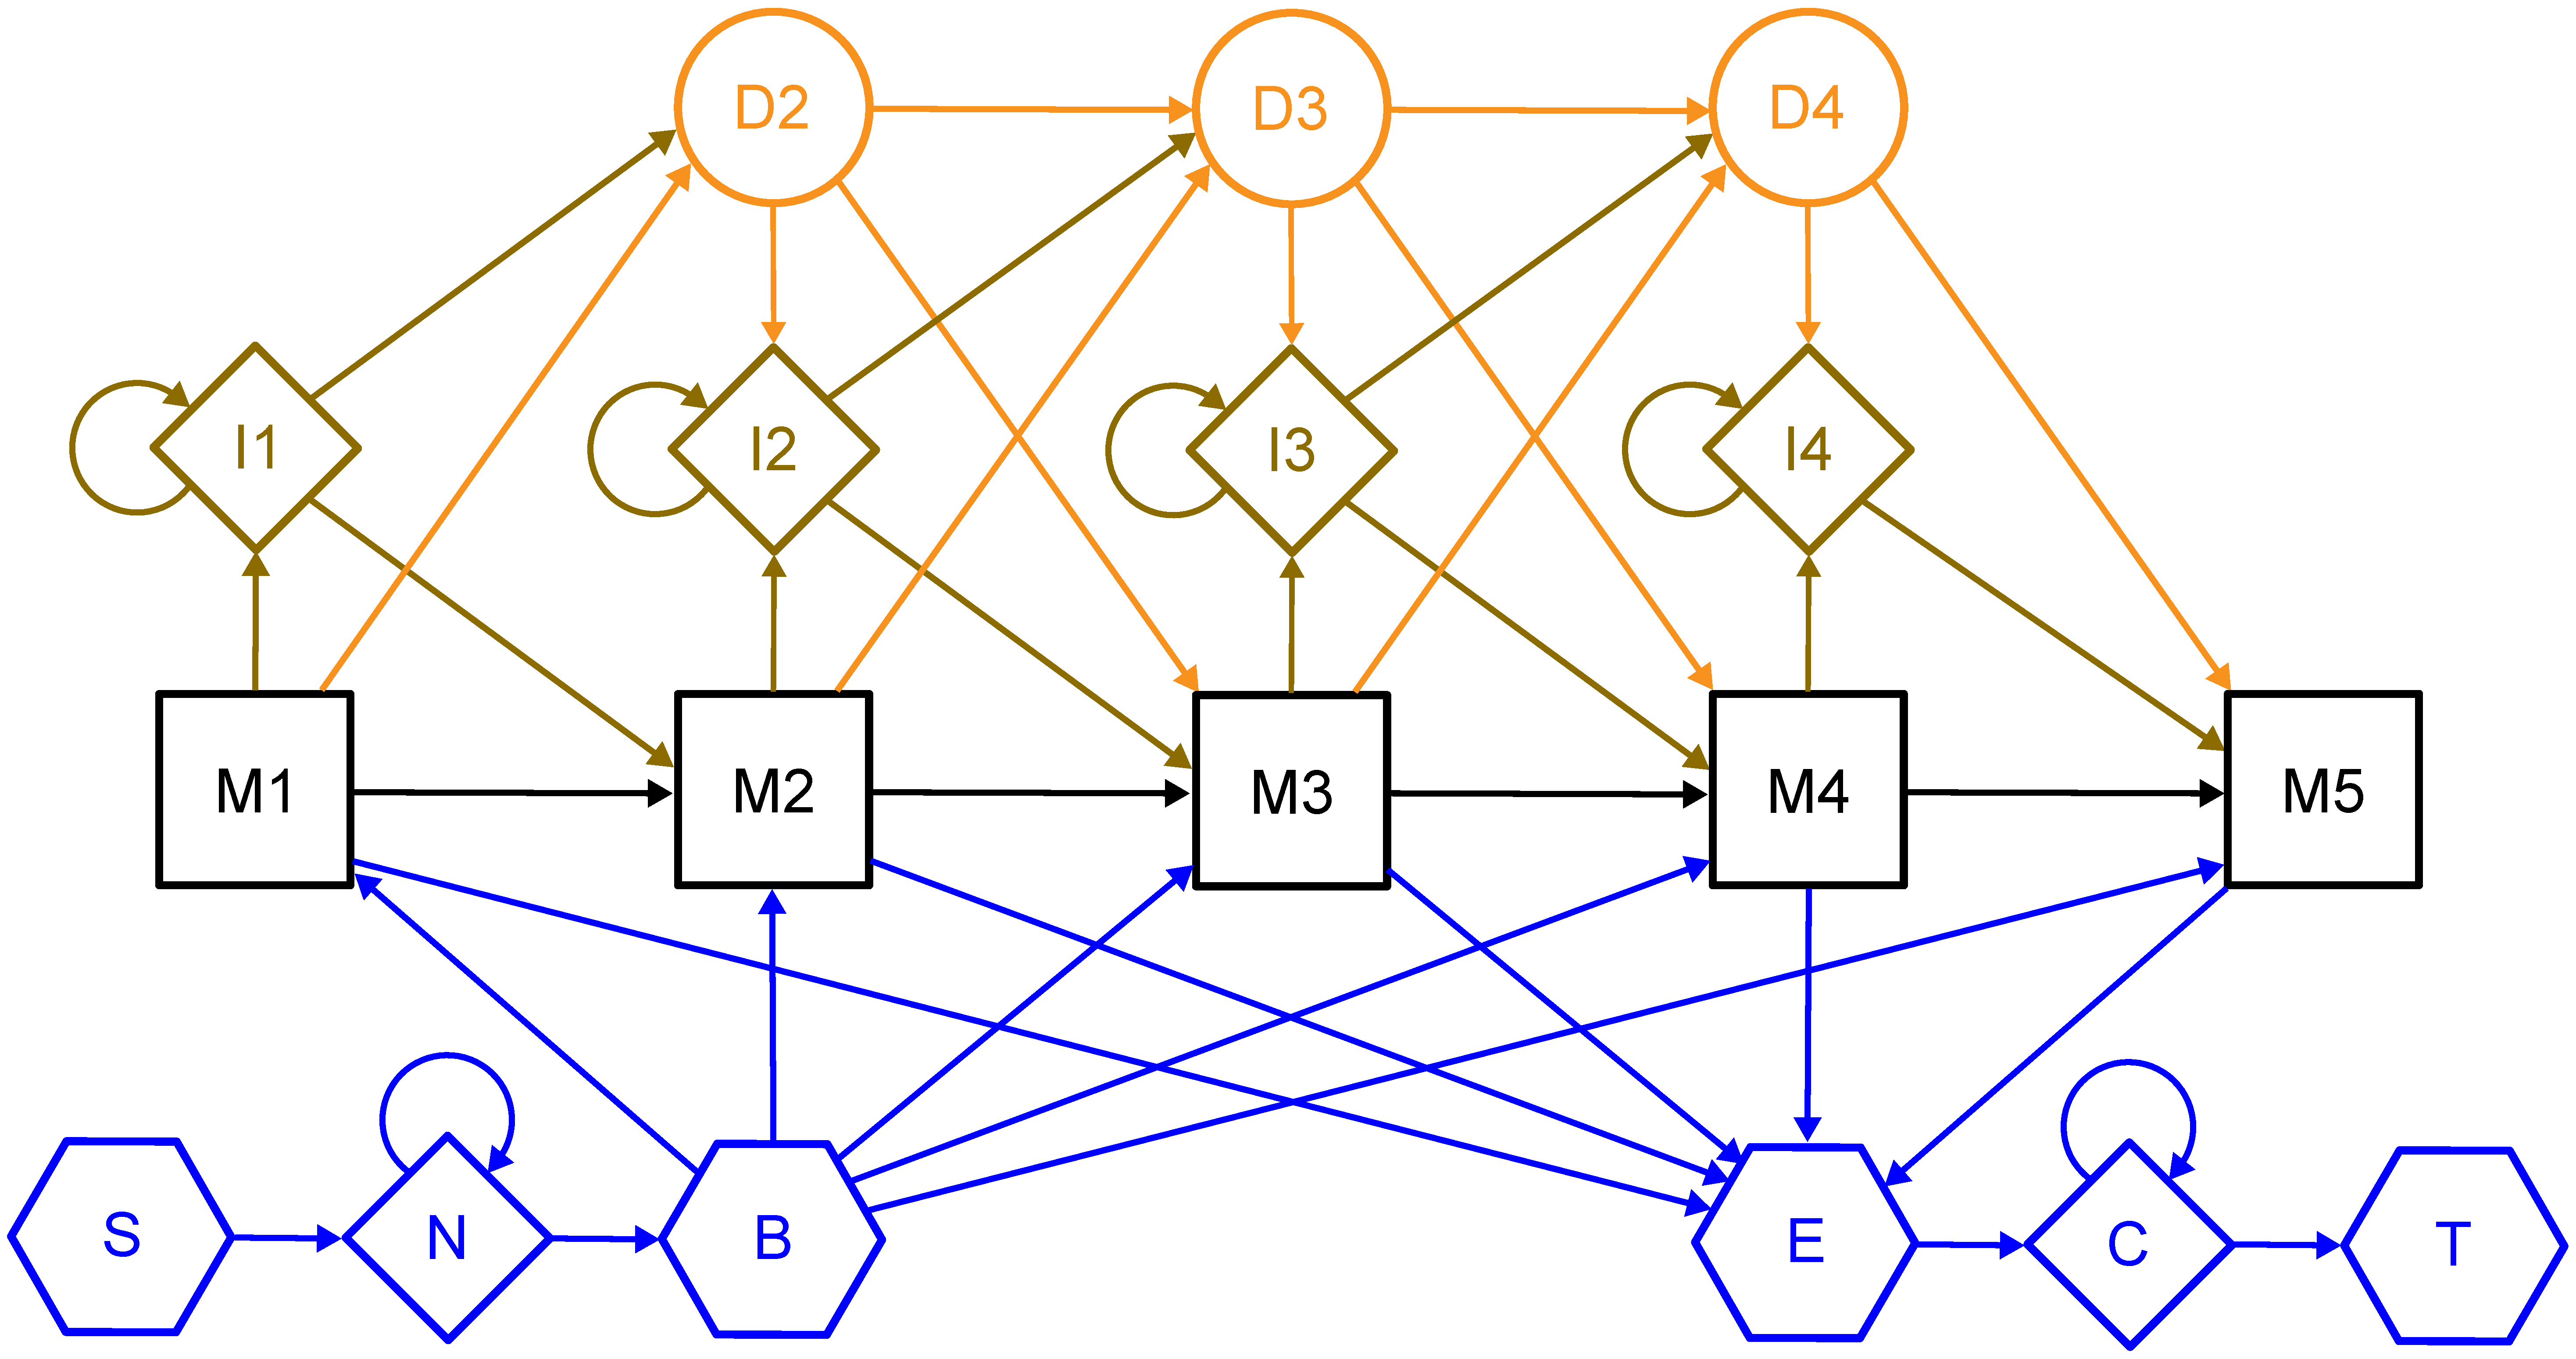
\includegraphics{img-hmm/model-local-unihit.eps} }
    \caption[HMM for unihit local alignment] {HMM for unihit local alignment (i.e. a single aligned region). }  
    \label{model-local-unihit}
  \end{center}
\end{figure}



\subsection{Extension of Profile HMMs to Multihit Alignments}

Up until now, it has only been discussed the case of \emph{unihit} evaluation with HMMs: only a single unbroken region, either the whole sequence and model (when in global alignment) or a subregion of the sequence and model (in the case of local alignment). It is also possible to use HMMs to match multiple regions, of both the sequence and the model. This is known as \emph{multihit} alignment mode, and it more closely resembles the classical alignment algorithms like Smith-Waterman. 

The previous HMMs can be extended to allow multihit alignments, by introducing another special state ('$J$'), connecting the $B$ and $E$ flanking states. This $J$ state requires only two parameters as well, a loop probability and a jump probability.

A multihit modeling capacity can be added to both global and local alignment HMMs. The \autoref{model-global-multihit} represents a HMM for multihit global alignment, while the more complex example for local alignment can be seen in \autoref{model-local-multihit}.

\begin{figure}[htb!]
  \begin{center}
    \resizebox*{1.0\columnwidth}{!}{ 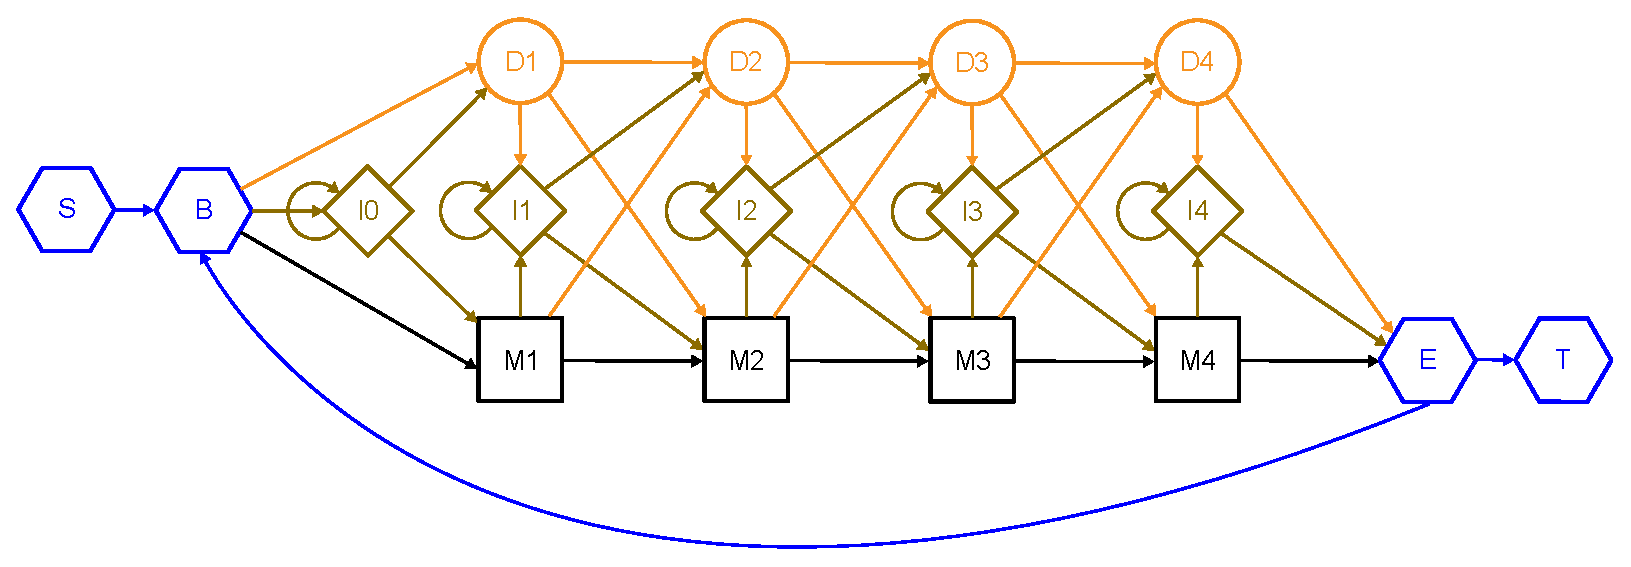
\includegraphics{img-hmm/model-global-multihit.eps} }
    \caption{HMM for multihit global alignment}  
    \label{model-global-multihit}
  \end{center}
\end{figure}


\begin{figure}[htb!]
  \begin{center}
    \resizebox*{0.9\columnwidth}{!}{ 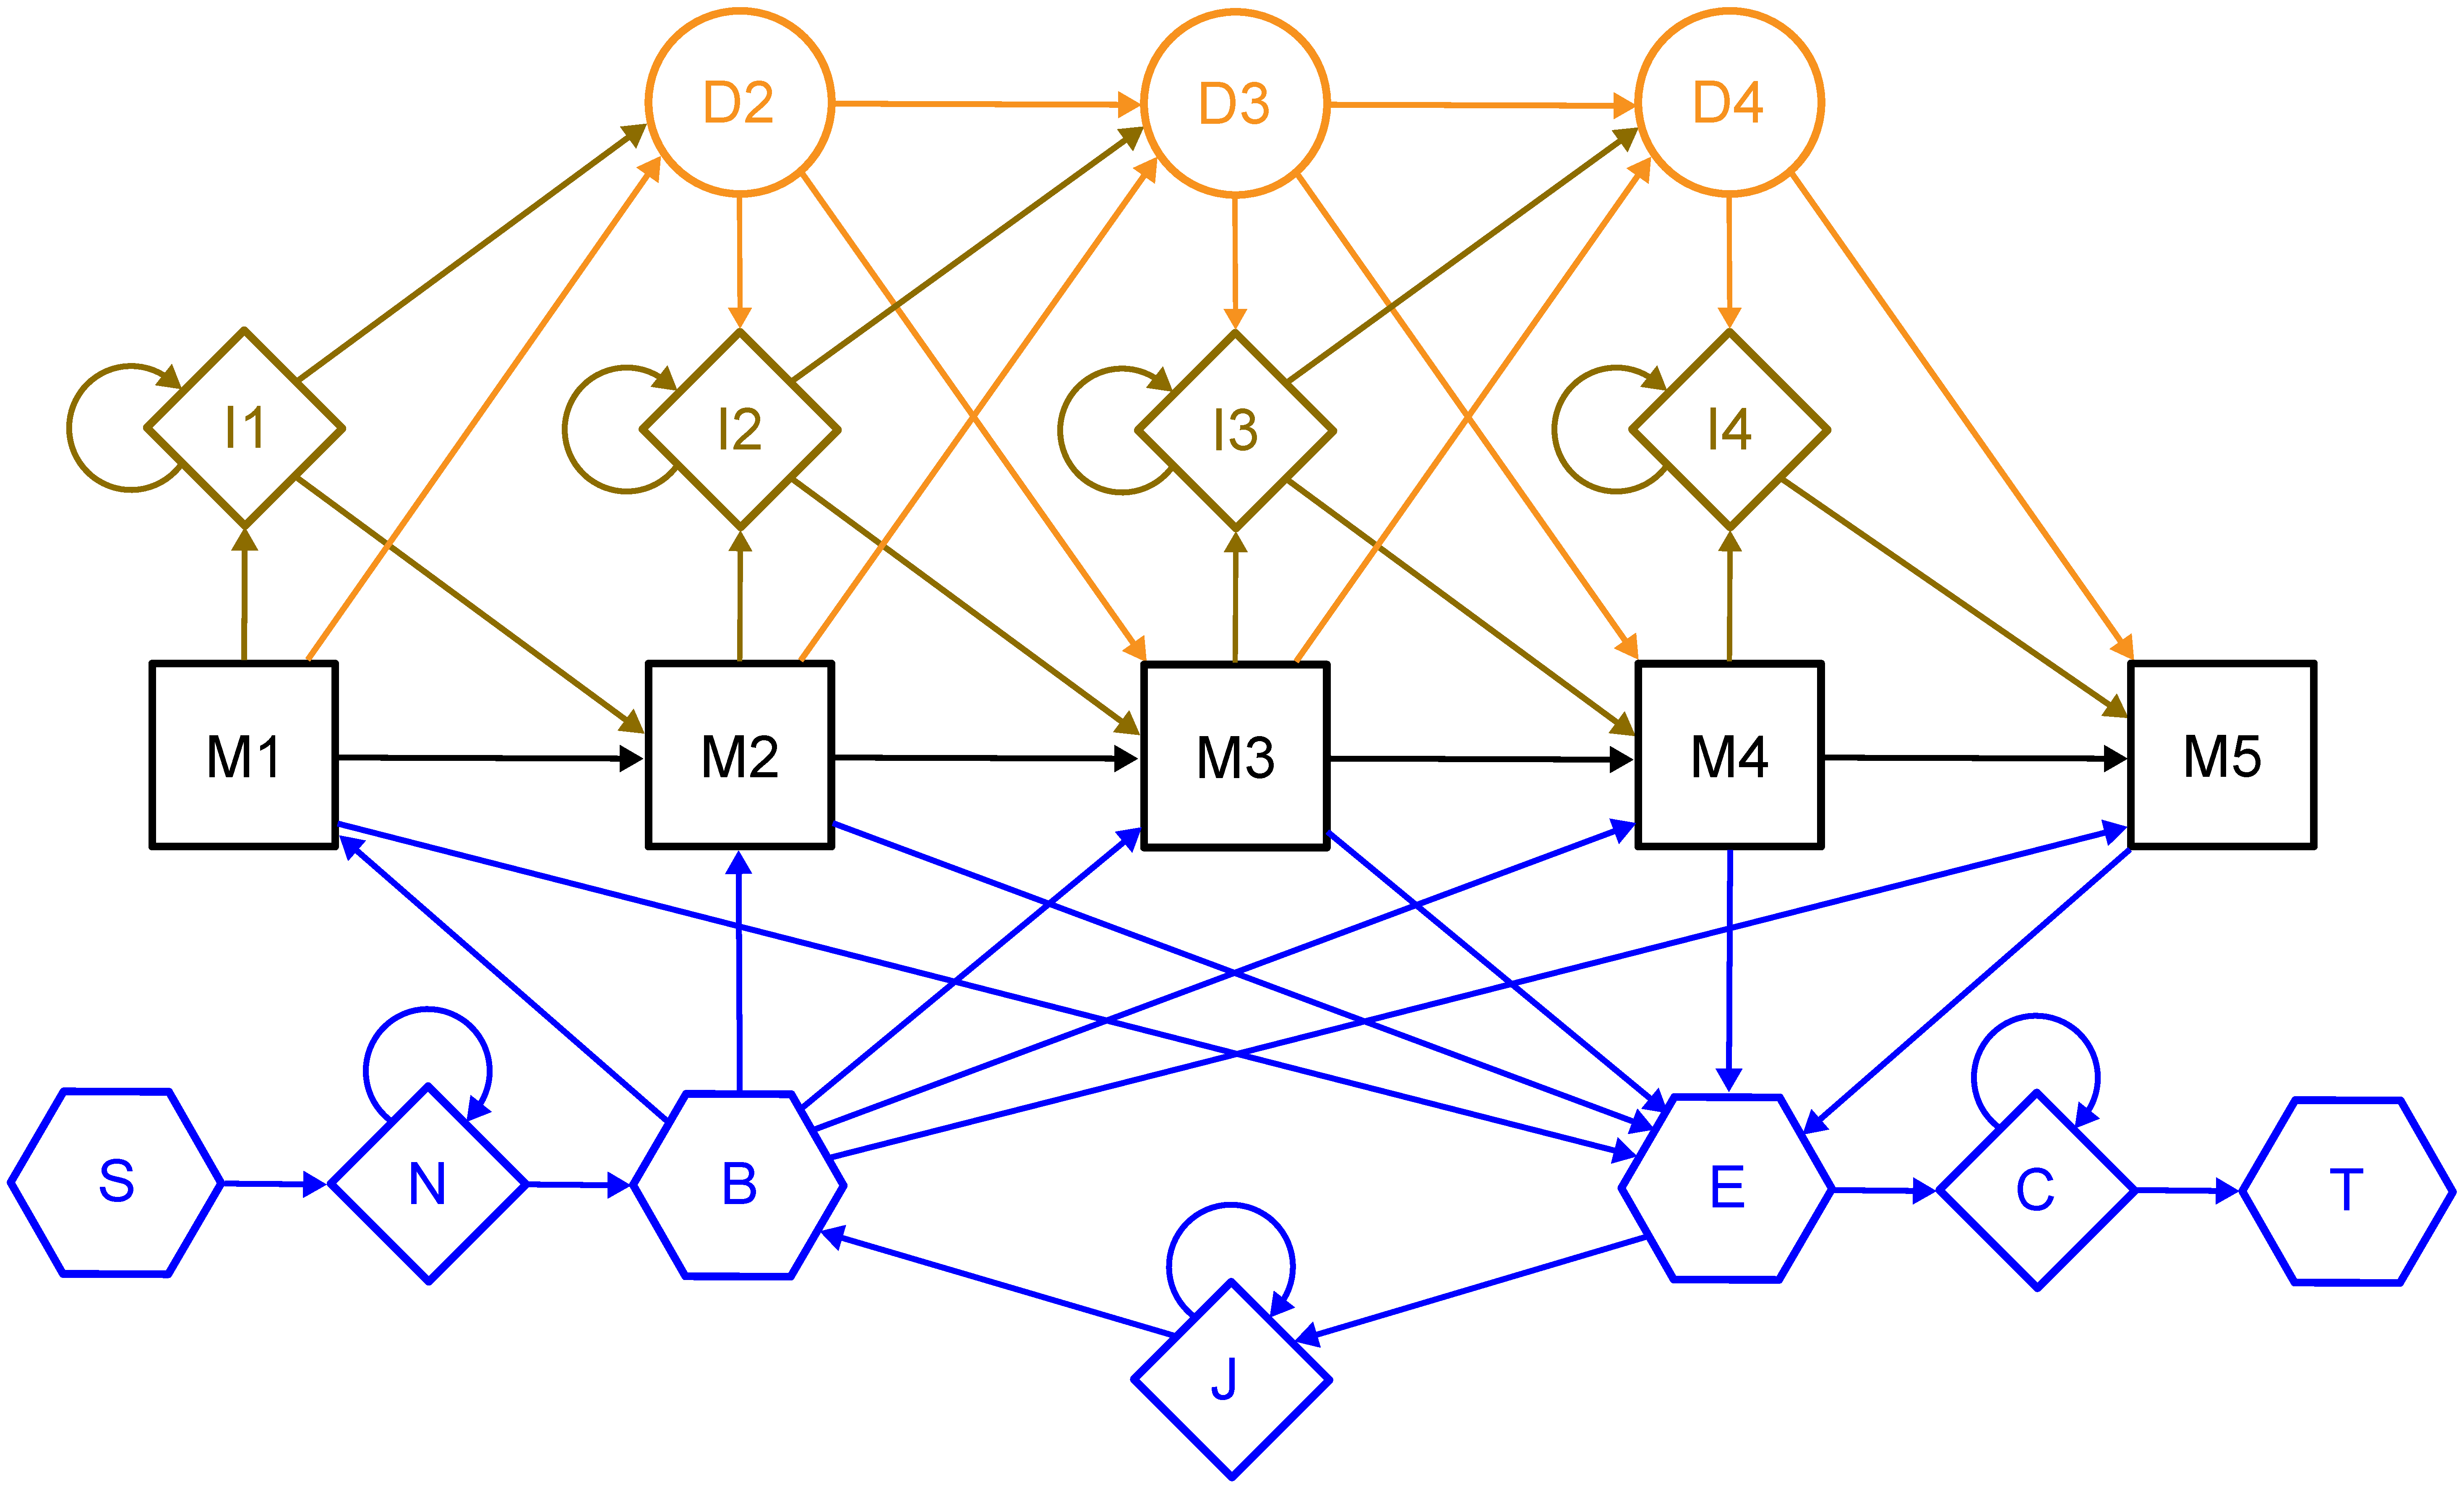
\includegraphics{img-hmm/model-local-multihit.eps} }
    \caption{HMM for multihit local alignment}  
    \label{model-local-multihit}
  \end{center}
\end{figure}

These multihit HMMs differ from the classical algorithms like Smith-Waterman and Needleman-Wunsch because the whole model is re-aligned against a new subregion of the sequence in each whole model loop. As a result, the same model region may be aligned multiple times to different sequence regions.

As for the algorithms to compute these multihit models, only the more interesting case of local alignment will be presented here.
The Viterbi algorithm for multihit local alignment can be computed by the pseudo-code in \cref{code-viterbi}.
The Forward algorithm for multihit local alignment model, with the additional special-states, is given by the pseudo-code in \cref{code-forward}.


%\cleardoublepage
\clearpage
 



%%%%%%%%%%%%%%%%%%%%%%%%%%%%%%%%%%%%%%%%%%%%%%%%%%%%%%%%%%%%%%%%%%%%%%%
%%%%%%%%%%%%%%%%%%%%%%%%%%%%%%%%%%%%%%%%%%%%%%%%%%%%%%%%%%%%%%%%%%%%%%%



%%%%%%%%%%%%%%%%%%%%%%%%%%%%%%%%%%%%%%%%%%%%%%%%%%%%%%%%%%%%%%%%%%%%%%%%%%%%%%%%%%%%%%%%%%%%%%%%%%%%%%%
% Parallelization of Homology Search
%%%%%%%%%%%%%%%%%%%%%%%%%%%%%%%%%%%%%%%%%%%%%%%%%%%%%%%%%%%%%%%%%%%%%%%%%%%%%%%%%%%%%%%%%%%%%%%%%%%%%%%

\fancychapter{Parallelization of Homology Search}

This chapter will review the most promising and well-studied techniques for parallelization of Homology Search, both of classical Alignment algorithms and Profile HMMs algorithms. The first section will deal with the parallelization of Alignment algorithms, and the later section will focus on the parallelization of Profile HMMs, which employ the same strategies, as it will be explained.

Parallelization approaches can be divided in Intra-task parallelism, wherein each alignment task is itself parallelized; and Inter-task parallelism, which consists of running multiple tasks (in this case, multiple alignments) in parallel.

\section{Parallelization of Alignment Algorithms}
\label{Parallelization of Alignment Algorithms}

\subsection{Instruction-level Parallelism and Code Optimization}

Scalar instruction-level parallelism in sequence alignment has been described by various authors such as Alpern \cite{alpern}, Szalkowski in SWPS3 (\cite {swps3}), Farrar \cite{farrarcell}, Rudnicki \cite{rudnicki2009cell}, \cite{rognes2011} and others. It is usually achieved by carefully re-arranging the instructions, normally done by the compiler or processor itself, in order to exploit the available processing pipelines on modern superscalar architectures. Special care must be taken on the implementation of very tight loops to allow the processor and compiler to better re-organize and parallelize the sequential code. The main concern is the removal of data dependencies and divergent execution paths (conditional branches).

Moreover, modern processors also employ many speculative optimization techniques, such as out-of-order execution and branch prediction. All these depend on the parallelization potential of sequential code, and as such, any un-parallelizable code section leads to a drastic performance cut. In particular, branch mis-predictions cause the whole pipeline to be flushed out, and all instructions already speculatively executed are discarded.

Another concern is the cache use: data locality is of the utmost importance, as well as the cache size itself, which determines how much of the inner variables and data can fit into cache. The cache size available, and the conscious and explicit optimization for such size, has a dramatic influence on the overall performance. A program with optimal cache utilization may come near a 100\% cache hit rate on the innermost loops that can fit into cache, and hence achieve an enormous speedup on the global runtime.

Many strategies have been described on this level to carefully hand-tune the most critical assembly code, such as:

- loop unrolling of the innermost loop \cite{alpern}, \cite{rognes2011}, so that it processes two or more iterations sequentially at a time. This reduces the number of inner branches, and hints the processor to parallelize the two iterations on the available concurrent execution pipelines;

- tiling of loops (strip-mining) to improve cache reuse \cite{alpern}. This technique consists of transforming a single loop into two nested loops, thus reducing the inner-loop length, to ensure that the inner-loop data stays in cache;

- reduce and remove any possible conditional branch, especially in the inner loops. In many cases, they can be moved out to the outer loops, initialization sections, or external same-level loops. This comes at the cost of some repeated or redundant work, but it is a small price to pay.
	



%%%%%%%%%%%%%%%%%%%%%%%%%%%%%%%%%%%%%%%%%%%%%%%%%%%%%%%%%%%%%%%%%%%%%%%
%%%%%%%%%%%%%%%%%%%%%%%%%%%%%%%%%%%%%%%%%%%%%%%%%%%%%%%%%%%%%%%%%%%%%%%

\subsection{Fine-grained Parallelism using SIMD units}

Fine-grained parallelism is implemented on the lowest instruction level. Besides the mechanisms described in the previous section, it can also be achieved through vector (SIMD) processing.

By now, SIMD extensions have already a reasonable long history of use and success. They implement a Single-Instruction/Multiple-Data parallel model on scalar CPUs, through the use of specialized vector processing units. Several of these instruction set extensions have enjoyed a considerable success, such as MMX/SSE on Intel and AMD's 3Dnow. One of most widely available is the SSE extensions on Intel processors. Each SSE register has 128-bits, capable of storing four 32-bit integers (rarely needed for alignment), eight 16-bit short integers (these can be used for alignments that reach high scores - such as very long sequences, very similar sequences, or very high base scores/penalties), or sixteen 8-bit bytes (the common case, allowing scores up to 255). Each stored element/value defines a single sequential 'execution channel'.

The first use of SIMD extensions for alignment tasks in general-purpose processors was employed by Alpern \cite{alpern} in 1995, using 64bit registers to simulate SIMD vectors. Others followed quickly,  using different parallelization strategies and decomposition patterns, on an increasing variety of different architectures (VAX mini-computers, Intel Pentiums, Cell BE, etc).


\subsubsection{Decomposition Patterns in Intra-task Parallelism}
\label{Decomposition Patterns in Intra-task Parallelism}

When employing SIMD vector processing, using each matrix cell computation as a \emph{primitive task}, the direction in which the cells are processed is of paramount importance. It determines how dependencies are parallelized, how many can be parallelized, and how costly it is to resolve the serial (non-parallelized) dependencies. When using SIMD units, the greatest obstacle is the dependencies within each SIMD vector (i.e. between the N parallel elements in the same N-channel SIMD unit vector). It is the most decisive factor in the overall performance.

Three main parallel decomposition patterns have been studied over the last decades to tackle the difficult problem of parallelizing data dependencies in intra-task parallelism: 

\myparagraph{Decomposition in a Diagonal Pattern}
\label{section-wozniak}

The most natural vectorial pattern to process the alignment matrix is by following the direction of the data dependencies, which is a diagonal direction \autoref{pattern-diagonal}. Processing each anti-diagonal in parallel is therefore a good method that was first proposed by Wozniak \cite{wozniak} in 1997 and often adopted ever since. One major advantage of this pattern is that it has no conditional branches in the inner loop. Still, it has one serious drawback: the heavy cost of the basic operations, required to diagonally access and process the matrix. Moreover, the diagonal pattern restricts the applicability of some precious optimizations, such as the the one proposed by Green in SWAT (see \sref{SWAT optimization}).

\myparagraph{Decomposition in a Vertical (or Horizontal) Continuous Pattern}
\label{section-rognes1}
		
Processing each column (or line) of the matrix in parallel is the other natural approach, perhaps the simplest and most intuitive \autoref{pattern-continuous}. This pattern has also been thoroughly employed, with some very optimized and efficient implementations, starting with Rognes \cite{rognes2000} in 2000 . The main problem of this strategy is the vertical (or horizontal, when parallelizing by lines) dependencies, which cannot be parallelized - they must be resolved sequentially, in a scalar way, amidst the SSE code, which is very inefficient.


\myparagraph{Decomposition in a Vertical (or Horizontal) Striped Pattern}
\label{section-farrar}

Building on Rognes solution, Farrar \cite{farrar} in 2007 devised a striped pattern decomposition to tackle the problem of vertical dependencies \autoref{pattern-striped}. Through the use of a striped pattern, beside the parallelization of horizontal and diagonal dependencies, it is also  possible to parallelize the vertical dependencies: each element j of the $i$-th segment will influence the same element j of the $(i+1)$-th segment. The biggest remaining problem is the dependencies across 'segment sections' (continuous sections) - in Farrar's algorithm, these are processed later, in a second inner loop (\emph{Lazy-F loop}), and following a SWAT-like optimization (i.e. the F values may only have any effect if they are higher than $W_1$). Despite the striped decomposition's better results, it is also less flexible and less prone to extension and customization (for instance, to run banded alignments). Moreover, for very short sequences, the striped pattern has an overhead (mostly from the Lazy-F loop) that is not easily amortized.

\begin{figure}[htb!]
\centering
\mbox{
	\subfigure[Decomposition in anti-diagonals. The lower, upper, and right sides are padded.]{
		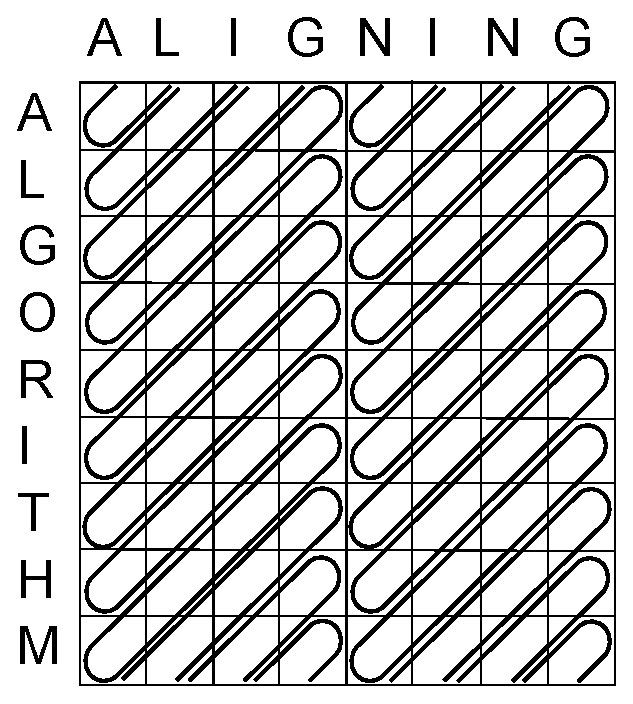
\includegraphics[scale=0.45]{img-par/pattern-diagonal.eps}
		\label{pattern-diagonal}
	}
	\quad
	\subfigure[Decomposition in continous lines. The lower side (last segment per column) is padded.]{
		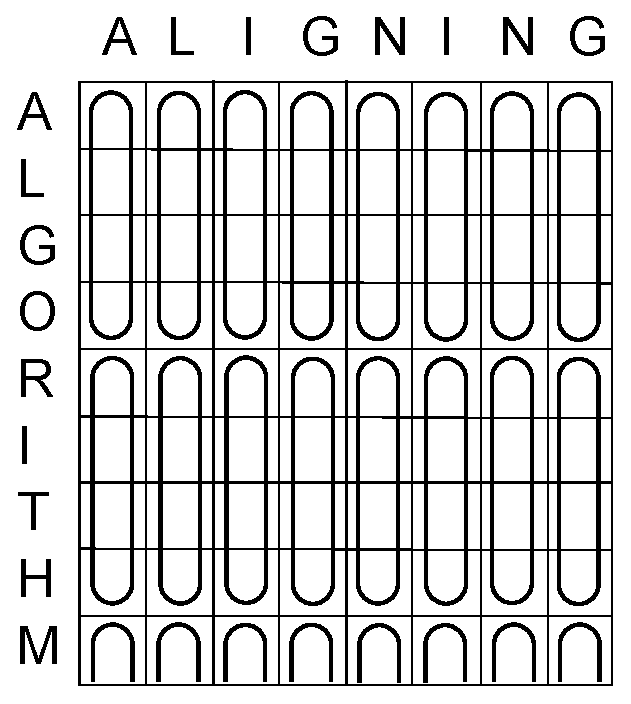
\includegraphics[scale=0.45]{img-par/pattern-continuous.eps}
		\label{pattern-continuous}
	}
	\quad
	\subfigure[Decomposition in striped lines. Each segment is padded.]{
		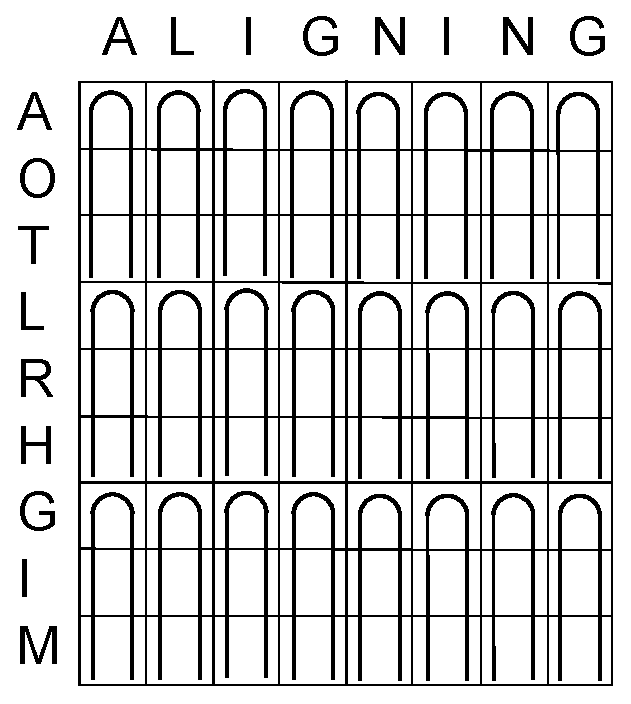
\includegraphics[scale=0.45]{img-par/pattern-striped.eps}
		\label{pattern-striped}
	}
}
\caption{Decomposition patterns for intra-task parallelism}
\end{figure}




%%%%%%%%%%%%%%%%%%%%%%%%%%%%%%%%%%%%%%%%%%%%%%%%%%%%%%%%%%%%%%%%%%%%%%%
%%%%%%%%%%%%%%%%%%%%%%%%%%%%%%%%%%%%%%%%%%%%%%%%%%%%%%%%%%%%%%%%%%%%%%%
		
\subsubsection{Main Problems of SIMD Intra-task parallelism}
		
There are several  issues afflicting SIMD algorithms, the most serious being:

\myparagraph{Limited Range of the parallel SIMD elements}

To maximize the algorithm's throughput, it is naturally desired to process as many elements in parallel as possible. This leads to fields of 8bits (1byte) for each element, which can have a maximum range of merely 255 (assuming only positive scores and penalties, or convert them to be such). For short sequences and reasonable typical scoring values, this is usually enough, but not always. Very similar sequences can easily overflow the 255-range, which invalidates the final score obtained, and forces alignment to be repeated with a higher range.
			
\myparagraph{Scoring matrices}

It is costly to access scoring matrices. Each access requires two indirections, one to find the sequence residue, and the other when the residue is used to access the matrix of scores. When using SIMD instructions, this problem increases tenfold - each vector element requires a different score, but those are scattered over the matrix (which is indexed by residue value, both in lines and columns).
	
\myparagraph{Divergent execution paths}

Divergent execution paths are  introduced by conditional branches in the inner loops, which in practice turn the theoretical parallel code into scalar code. Furthermore, these hamper the processor's pipeline and branch prediction. One example is the required branches when processing the vertical dependencies within a SIMD vector.

\myparagraph {Scalar sequential code}

Some inherently scalar sequential code cannot simply be parallelized. For instance, the vertical dependencies cannot be fully parallelized, as well as the initialization scalar values. These singular cases require manipulation of the internal SSE elements with cumbersome vector instructions, such as shifts, packs and shuffles, to simulate simple scalar operations.

\myparagraph {Cache Storage}

A fundamental issue is the cache availability to store the arrays of SSE vectors used in the innermost loops: one E array, one of two H array(s), the F value, several auxiliary variables and constant values (variable names taken from Gotoh's equations, see \sref{Gotoh algorithm}). A lazy tuning of the inner loops data to the cache storage size may considerably impair the overall system performance.

\myparagraph {Banded Alignment}

Banded alignment brings new challenges to vectorial parallelism. Farrar's striped pattern works very well for long runs, but the Lazy-F loop overhead becomes a problem in very small runs (a band width of 30 bases can fit entirely in two SSE vectors). Another problem is the frequent inner-loop re-initializations. 
%TODO MAIS COISAS
Regarding the query profiles, their loading onto the SSE registers also induces an additional problem, since the memory becomes unaligned when processing each new column starting one cell later.
	
	
\subsubsection{Improvements for SIMD Algorithms}

To solve these main problems and improve the SIMD implementations, a few clever optimizations have been proposed:

\myparagraph{Unsigned and Saturated Arithmetic}

In order to increase the SIMD elements available range, unsigned arithmetic can be used, thus doubling the maximum range.

To deal with negative values, all scores and matrix cells are biased by a fixed small amount that guarantees no negative scores. Saturated arithmetic is then used to prevent values from dropping below 0 (and underflowing), as well as capping the values at the maximal value, preventing overflows. The minimum operation of the \ac{SW} algorithm is also spared, being replaced by the implicit sature-to-zero operation. Underflows correspond to the maximum operation with 0, and are part of the algorithm. Overflows, on the contrary, are an error introduced by the limited range used, and are used as a sign that the whole procedure needs to be repeated with a higher range. As such, the test for the correctness of the alignment needs only to be done in the end, and it is simply '\emph{final score \textgreater MaxValue - Bias}'.

There are cases however, when this mechanism cannot be used, as necessary architectural support is lacking. For instance, SSE only supports  signed arithmetic for short values (16bit). To overcome this obstacle, some emulations of unsigned saturated arithmetic were devised. Farrar biased all values with -32k (the short min value), and then used saturated signed arithmetic to solve the problem. Rognes \cite{rognes2011} in 2011 used a similar approach in the 7bit range, with both saturated arithmetic and unsaturated maximum, to avoid the Add instruction needed to unbias the scores.
		
For architectures without any support for saturation, Farrar \cite{farrarcell} proposed a different biasing procedure. The idea is to add a small bias to every value, maximize each computed value with this bias (preventing it from dropping below 0), and testing for overflow with '\emph{value \textgreater MaxValue - Bias}'.

\myparagraph{Query-specific scoring profile}
\label{scoring-profile}

Packing each element at a time into the required SSE vector would be a considerable bottleneck. To avoid this, the substitution scores must be stored sequentially (or striped in Farrar's version) in memory, according to the respective sequence elements, so that a single load instruction can fetch the whole SSE vector from the substitution matrix in memory onto a register. The result is a new scoring matrix adapted to the query sequence, called a query-specific scoring profile.

The storage required for such a profile can also easily grow out of hand, especially for very large queries. This is a serious problem in computers with very small on-chip memory (GPUs and Cell's synergistic processors, for instance). The mechanism described in the next paragraph attempts to minimize this problem. 
		
\myparagraph{Compacting and expanding scoring profiles}

A possible method to compact the scoring profile was proposed in \cite{swps3}. The idea is to use the minimum required memory to keep the substitution scores (normally only 1byte per value), and expand them to larger sizes using SSE's unpack instruction, when executing with 16bit of higher elements' ranges. The sequences themselves can also be compacted with 2bits per base. 

%\myparagraph{Scaled Offset Map}
%A recent original ideia has been presented \cite{scaledmap} 
%A possible strategy to support much larger scores, while still using the same limited 8bit elements, is the usage of a scaled offset map. It consists of a checker-block divided matrix with offset factors to represent higher-ranged scores. Each square block of the \ac{DP} matrix keeps an offset scale coefficient that gives a constant offset for the scores of the whole block when multiplied by a constant offset base value. This offset scale is determined at the boundaries between blocks, such that no possible variation within the same block can surpass the constant offset base.

%This mechanism introduces an overhead in the blocks' boundaries, as well as more storage needed to keep the offsets, so it is only useful when most alignments run in the limited range with a small but still considerable fraction needing higher ranges.
% When most alignments need the 16bit range, it is also not practical to use this, since it entails the overhead... ERRADO o overhead  e' constante independente das scores
	
\myparagraph{Optimizations of the Lazy-F loop}

Some optimizations have been studied for Farrar's Lazy-F loop \cite{swps3} \cite{farrarcell}, and achieved good results. One of the improvements consists mainly on relaxing the loop termination condition, since the original Lazy-F loop has in the worst case N (the complete column length) iterations. The other idea is moving some of the conditionals to a more external (and hence, less executed) position.

%estudar e expandir isto



\subsubsection{SIMD Implementation of Global Alignment}

As it has been described in \sref{Smith-Waterman algorithm for Local Alignment}, global alignment (in particular the \ac{NW} algorithm) differs from local alignment (\ac{SW}) in that the alignment must cover the whole sequences instead of just partial, positive-scoring, subsequences. Global alignment can be regarded as subproblem of local alignment when the start and end point of the alignment are fixed. The \ac{NW} algorithm, being a somehow reduced form of the \ac{SW} algorithm, is also and more efficient and simpler to implement. The main differences in the implementation are the following:
	
- No need to keep the best score found. The resulting alignment score is always the score of the last (rightmost) cell. A maximum operation in the inner loops is thus spared
	
- No need to use a zero lower bound - the maximization with 0 is also avoided.

- No alignment re-runs due to overflowing: Considering that, increasing scores can be used instead of decreasing, the values' range will always be positive; hence there are no underflows and lower-bound saturation is not needed. Higher-bound saturation is still needed to avoid wrap-around's. However, the overflown cells no longer constitute a problem since they have an extremely poor score (the higher the cell value, the worse it is). They are merely an innocuous side-effect of the procedure. In principle, they will never be chosen by the recursion's rule, and thus can be safely ignored. Actually, this may not be always the case, if the used arithmetic range is very ill-adjusted to the sequences. For correctly parametrized alignments, this technique can generally be safely used.
	
- Given that the start and endpoints of the alignment are known, some tuning of the algorithm can be done (for instance, heuristic filters and metrics).	%EXPANDIR MAIS ISTO
	
% TODO => Varios optimizacoes possiveis das implementacoes SW estudadas, qd passadas a globais




%%%%%%%%%%%%%%%%%%%%%%%%%%%%%%%%%%%%%%%%%%%%%%%%%%%%%%%%%%%%%%%%%%%%%%%
%%%%%%%%%%%%%%%%%%%%%%%%%%%%%%%%%%%%%%%%%%%%%%%%%%%%%%%%%%%%%%%%%%%%%%%

\subsection{Intra-task Parallelism on Multiple Cores}

Middle-level parallelism is achieved by dividing the \ac{DP} matrix in 'chunks' that can then be processed in parallel by the different cores on a single machine. This can also be extended to a grid of compurers, with each node processing a chunk, when the sequences are quite large. Several recent applications have been developed using this paradigm (\cite{liao2004parallel}, \cite{meng2005exploiting}, \cite{framework2010parallel}, \cite{hosny}).

This middle-level approach is much easier to implement than the fine-grained SSE: this one follows a simple MIMD model, in which each single processing datapath can diverge without any penalty, contrary to the SIMD model of vector processing that binds all the datapaths together. 

The first issue to consider in this level is the order in which the chunks are processed. Which ones can be processed in parallel? How many at the same time? The strategy that seems to work best is by parallelizing along each anti-diagonal (similar to Wozniak's fine-grained pattern \cite{wozniak}), which is the natural direction of the algorithm's dependencies. This leads to a so-called "tiled-chunk pattern" (each diagonal of chunks being seen as a tile). Authors in \cite{boukerche2007parallel}, \cite{zalign} and \cite{hosny} use this pattern. The order in which the chunks are processed is not very strict: they can advance vertically or horizontally. The only restriction is that each chunk above and to the left must be processed before.

To minimize the communication cost of exchanging values between cores, each one should process a chunk as large as possible in each iteration. The best layout is to use a single chunk per process per level (communication round). Each chunk should have roughly close to $\frac{N}{P}$ columns (or rows vice versa, $N$ columns, $P$ processors) , so that the computational work is balanced among all cores.  As for rows, each chunk can have any number of them. In particular they can have only one row, allowing for a finer-grain parallel decomposition \cite{boukerche2007parallel} (especially useful when the communication cost is low, such as when using shared symmetric memory multiprocessors). Note that the score matrix is an abstract concept: in practice the Gotoh linear-space algorithm is always employed, and only a couple of arrays are needed.

When using a granularity of one for columns and rows (1 cell for each chunk), each diagonal only depends on the past two diagonals (the previous one for vertical and horizontal dependencies, and the other for the diagonal dependencies). When using larger chunks, the data requirements are much better: each diagonal front needs only a 'stair-shaped' previous diagonal chunk-frontier (with $M+N$ cells, $M$ columns, $N$ rows). Since each diagonal has $a \times N$ cells (arbitrary granularity, $a$), the needed data-to-computation ratio is quite good. On the other hand, the higher the granularity is, the slower becomes the initial start-up time when some cores are idle waiting for available chunks.

Several alternative algorithmic strategies have been proposed to decompose the matrix between workers (such as ParAlign \cite{paralign} and GCM-BSP \cite{parbcp}). These use exploitable properties of the algorithms to split the computing space among parallel nodes, and later merge the results, usually with some restriction or accuracy loss. Most of these algorithms also only work for global alignment, since the 'restarting' step of local alignment is much more unpredictable.

% (EXPANDIR ESTAS TECNICAS)


%%%%%%%%%%%%%%%%%%%%%%%%%%%%%%%%%%%%%%%%%%%%%%%%%%%%%%%%%%%%%%%%%%%%%%%
%%%%%%%%%%%%%%%%%%%%%%%%%%%%%%%%%%%%%%%%%%%%%%%%%%%%%%%%%%%%%%%%%%%%%%%

\subsection{Inter-task Parallelism}
\label{Inter-task Parallelism}

Besides parallelizing a single alignment task, it is also possible to process multiple alignment matrices in parallel too (a single cell, or chunk, of each matrix at a time). This alternative method has also been much studied in the last decade.


\subsubsection{SIMD extensions}
\label{Rognes-section}

Instead of using a SIMD vector to process multiple cells of the same alignment matrix, we could feed a single cell from multiple matrices to each one of the independent parallel channels. This approach was first proposed by Alpern \cite{alpern} in 1995, and later extended and improved by Rognes in 2011 \cite{rognes2011}, on SSE.

Rognes thought of using vector processing such as SSE to implement inter-task parallelism (i.e. running many alignment tasks in parallel), using a lock-step processing model. Each vector is loaded with N different sequences, one in each vector element (or channel), and the algorithm aligns them concurrently against a target sequence, using the N vector channels to hold the independent computed values. 

The main advantage of using parallel channels is the complete elimination of all data dependencies among SIMD elements. The alignment tasks are completely independent.

The drawbacks of this strategy are its restrictive applications and limitations, deriving from the fact that the N alignments proceed on step from begining to end. Any divergence on the program flow carries a prohibitive performance penalty, either as stoppage time or as wasted computing potential (for instance, empty padded cells).

One problem is the necessary pre-loading and arrangement of the per-residue emission scores. The emission scores to use depend on the searched sequences, and thus cannot be predicted, pre-computed and memorized before knowing those sequences. Each new batch of N sequences to search requires the loading of new emissions scores.

Rognes solution is to load the emission scores for the N different residues from the N database sequences, each from its own emission scores' array, before the inner loop through the query. The emission arrays are thus loaded for the N new residues to process, and transposed from the original continuous pattern into a striped pattern, using the SSE operations unpack and shuffle. After the transposition, each new SSE vector then holds N single emission scores from the different N residues, all of which corresponding to a single query residue.

Another problem is the different lengths of the N concurrent database sequences. Rognes' solution is to stop the algorithm whenever one of the sequences ends, and replace it with another in the same channel. An alternative way would be to pre-sort the whole database by sequence length, and thus minimize the length differences in each run of the algorithm. The total cumulative length differences could be so small as to become negligeble, and so the wasted computed cells could be easily ignored.



\subsubsection{Multiprocessors}

Using a MIMD model for inter-task parallelization is much simpler, and more flexible. The sequences to align are divided by the different scalar processing units, which can be threads on a multicore or processes in separate machines. Intuitively, for smaller sequences, it is more convenient and efficient to use a single multicore processor to reduce communication costs, while for larger alignments, a grid of machines offers more available memory and resources. When compared to SIMD inter-task parallelism, this strategy is much less constrained, and supports larger sequences.

Load balancing is also an important issue: the overall sequence load for each node should be roughly identical. For this purpose, the sequences may be first sorted by length, and then 'horizontally' divided among the nodes.

% TODO extender isto





%%%%%%%%%%%%%%%%%%%%%%%%%%%%%%%%%%%%%%%%%%%%%%%%%%%%%%%%%%%%%%%%%%%%%%%%%%%%%%%%%%%%%%%%%%%%%%%%%%%%%%%
%%%%%%%%%%%%%%%%%%%%%%%%%%%%%%%%%%%%%%%%%%%%%%%%%%%%%%%%%%%%%%%%%%%%%%%%%%%%%%%%%%%%%%%%%%%%%%%%%%%%%%%
%%%%%%%%%%%%%%%%%%%%%%%%%%%%%%%%%%%%%%%%%%%%%%%%%%%%%%%%%%%%%%%%%%%%%%%%%%%%%%%%%%%%%%%%%%%%%%%%%%%%%%%
%%%%%%%%%%%%%%%%%%%%%%%%%%%%%%%%%%%%%%%%%%%%%%%%%%%%%%%%%%%%%%%%%%%%%%%%%%%%%%%%%%%%%%%%%%%%%%%%%%%%%%%


\section{Parallelization of Profile Hidden Markov Models}

Here, the most studied and promising parallelization strategies for Profile HMMs will be discussed, building upon the methods for classical alignment algorithms, already described in section \sref{Parallelization of Alignment Algorithms}. As has been shown in the last section, the HMMs algorithms (Viterbi and Forward) have a similar structure and data access pattern as the classical single alignment algorithms (Smith-Waterman, Needleman-Wunsch etc). As would be expected, this similarity in the algorithms makes the parallelization strategies of single alignment to be very fitting for HMMs as well.


\subsection{Comparison between Profile HMMs and Single Alignment algorithms}

The algorithms used for Profile HMMs (Viterbi and Forward) are largely similar to the single alignment algorithms that were presented first (Smith-Waterman and Needleman-Wunsch with the Gotoh Optimization, see \sref{Gotoh algorithm}). They both are Dynamic Programming algorithms with three components to model Matches/Mismatches, Insertions and Deletions. They both have the same recursive dependencies, such as, horizontal, vertical and diagonal.

To compare them, these are the Gotoh Recursions for the Smith-Waterman single-alignment algorithm:

match   $ M(i,j) = Max \begin{cases} 
						0 		\\
						M(i-1,j-1) + weight(a_i; b_j)	\\
						I(i,j)	\\
						D(i,j)	\\
						\end{cases} $ \\
\\

insert $ I(i,j) = Max \begin{cases} 
						M(i-1,j) + Wext + Wopen \\
						I(i-1,j) + Wext		\\
						\end{cases} $ \\
\\

delete $ D(i,j) = Max  \begin{cases} 
						M(i,j-1) + Wext + Wopen \\
						D(i,j-1) + Wext 	\\
						\end{cases} $ \\
\\
And these are the three main recursions of the Viterbi algorithm for a Profile HMM that suppors local alignment, in log-space, using a similar notation and ignoring the other special states for now:

match	$ M(i,j) = log\ {e_{Mj}(x_i)} + Max  
				\begin{cases}
					B(i-1)     + log\ t_{B_{j-1} M_j} \\
					M(i-1,j-1) + log\ t_{M_{j-1} M_j} \\
					I(i-1,j-1) + log\ t_{I_{j-1} M_j} \\
					D(i-1,j-1) + log\ t_{D_{j-1} M_j} \\
				\end{cases} $ \\
\\

insert	$ I(i,j) = Max 	\begin{cases}
					M(i-1,j) + log\ t_{M_{j} I_j}	\\
					I(i-1,j) + log\ t_{I_{j} I_j}	\\
				\end{cases} $ \\
\\

delete	$ D(i,j) = Max	\begin{cases}
					M(i,j-1) + log\ t_{M_{j-1} D_j} \\
					D(i,j-1) + log\ t_{D_{j-1} D_j} \\
				\end{cases} $ \\ 
\\
It should be remembered that the transitions and emissions scores ($ log\ t_{X_j' Y_j} $ and $ log\ {e_Mj(x_i)} $) are pre-computed scores, which depend solely on the sequence symbol (in the case of emissions) and the transition states (in both cases).
It is thus clear that these two algorithms have are very much alike, and can be computed with roughly the same methods. The same holds true for the Forward algorithm, although with the particular table lookups.

Now, it is relevant to consider and contrast the differences between the two types of algorithms:

\begin{enumerate}

\item Gap Scores: While Smith-Waterman uses two single constant values, respectively for opening and extending a gap; Viterbi uses a series of constant values dependent on the position-specific transition states. This series of values introduces a necessary lookup in an array, and thus an unavoidable delay.


\item Match scores: Smith-Waterman uses a Weighting matrix, also known as a 'scoring matrix' (such as BLOSUM \cite{blosum} and PAM \cite{pam}), accessed by a combination of the target symbol and query symbol. The weighting matrix can be optimized into a query-specific Scoring Profile (see \sref{scoring-profile}), yielding a single continuous array of scores for each inner-loop iteration.
	The rough equivalent in the Viterbi case are the Match emission scores, which vary according to the current Match State $M_j$ and sequence symbol. Thus they are already in a 'model-specific profile', and can be re-used between sequences, essentially like a Query-Specific Profile for the Smith-Waterman.


\item Data dependencies:
\begin{enumerate}
\item In the SW algorithm, the I values depend solely on the last column, the D values on the last line, and the M values on the current I and D values, plus the previous diagonal M value. The computations can be re-ordered to use a single array for the I and M values, and a single cell for the D values (as per the Gotoh optimization). Although most authors use two switching arrays for the M values (for the current and last columns), it is possible to dispense one of them by doing delayed stores, i.e., loading the next $M(j)$ before storing the current $M(j)$. The re-ordered computations follow the scheme in \cref{code-sw-delayed-stores}.


\begin{algorithm}[htb!]
\caption[Smith-Waterman pseudo-code with delayed Match writes] {Pseudo-code of the Smith-Waterman algorithm with delayed Match writes}
\label{code-sw-delayed-stores}

\begin{algorithmic}

\For{$i \gets 1 \textrm{ to } TargetLength $} 

	\State	 $ D \gets Mprevious \gets 0 $

	\For{$j \gets 1 \textrm{ to } QueryLength $} 

		\State // Use of delayed \emph{H(i-1,j-1)} value, i.e., \emph{Mprevious}; and update in-place of \emph{D} 
		\State $ D \gets Max 	\begin{cases} 
									 Mprevious + Wext + Wopen	 	\\
									D + Wext 					\\
								\end{cases} $ \\
		\State // Update in-place using the values of \emph{I(j)} and \emph{M(j)} from the \emph{i-1} outer-loop iteration 
		\State $ I(j) \gets Max	\begin{cases} 
										M(j) + Wext + Wopen	\\
										I(j) + Wext			\\
									\end{cases} $ \\
		
		\State // Use of delayed \emph{H(i-1,j-1)} value, i.e., \emph{Mprevious} 
		\State $ Mnew \gets Max \begin{cases} 
									0 		\\
									Mprevious + weight(Target_i; Query_j)	\\
									I(j)	\\
									D		\\
								\end{cases} $ \\
		
		
		\State $ Mprevious \gets M(j) $		// Save \emph{H(i-1,j)} for next iteration 
		\State $ M(j) \gets Hnew $ \ \ \ \ \ \ \ \ // Delayed store of \emph{H(j)} 

	\EndFor
\EndFor

\end{algorithmic}
\end{algorithm}


\item In the Viterbi (or Forward) algorithm, the data dependencies are more complex but they can also be implemented with single I and M arrays, using delayed load/store operations. As for the D dependencies, they now require a whole array instead of a single variable, since the previous D column ($D(i-1,j-1)$) has to be saved for the computation of the match states ('M'). The resulting re-ordered computations are shown in \cref{code-viterbi-delayed-stores} (all scores are in log-odds).


\begin{algorithm}[htb!]
\caption[Viterbi pseudo-code with delayed Match writes] {Pseudo-code of the Viterbi algorithm with delayed writes of the Match values. All scores are represented in log-odds.}
\label{code-viterbi-delayed-stores}
\begin{algorithmic}

\For{$i \gets 1 \textrm{ to } TargetLength $} 

	\State	 $ D \gets Mprevious \gets 0 $

	\For{$j \gets 1 \textrm{ to } QueryLength $} 

		\State // Use of delayed values from last iteration
		\State $ Mnew \gets e'_{Mj}(x_i) + Max  
					\begin{cases}
						B     		+ a'_{B_{j-1} M_j} \\
						Mprevious	+ a'_{M_{j-1} M_j} \\
						Iprevious	+ a'_{I_{j-1} M_j} \\
						Dprevious	+ a'_{D_{j-1} M_j} \\
					\end{cases} $ \\
		
		\State // Preemptive Load of previous values, from the \emph{i-1} outer-loop iteration
		\State $ Mprevious \gets M(j) $
		\State $ Dprevious \gets D(j) $
		\State $ Iprevious \gets I(j) $
		
		\State // Delayed Store of new values
		\State $ M(j) \gets Mnew $
		\State $ D(j) \gets Dnew $
		\State $ I(j) \gets Max
						\begin{cases}
							Mprevious + a'_{M_{j} I_j} 	\\
							Iprevious + a'_{I_{j} I_j}	\\
						\end{cases} $	\\

		\State // Preemptive Computation of \emph{D(i,j+1)}, to be stored in the next iteration
		\State $Dnew \gets Max
						\begin{cases}
							Mnew + a'_{M_{j-1} D_j} 
							Dnew + a'_{M_{j-1} D_j} 
						\end{cases} $
	\EndFor
	
\EndFor

\end{algorithmic}
\end{algorithm}

\end{enumerate}
\end{enumerate}

So, to surmise, the Viterbi algorithm requires more complex dependencies, with more delayed load/stores, and using more memory (state-specific transitions scores and a 'D' array).



\subsection{Intra-task parallelization of Profile HMMs}

Since the Viterbi and Forward algorithms for Profile HMMs are so similar to the Smith-Waterman algorithm, it can be used the same parallelization strategies described before for Single Alignment. These can be divided in intra-task (parallelizing each task in itself, each execution of the algorithm) and inter-task approaches, also known as 'data-parallelism' (running multiple tasks concurrently, i.e. executing the algorithm concurrently on different data sequences).

Intra-task parallelism has been the most used on SIMD architectures (such as SSE). Lindahl in 2005 \cite{lindahl} used a continuous pattern (as in \sref{section-rognes1}) on the AltiVec SIMD instruction set. Lindahl also unrolled the inner loop, producing 24 intermediate values to make better use of the available AltiVec registers, interleaved computations with memory fetches to hide some memory latency.  % achieving a 9-fold speedup. nao percebo como...

The most successful decomposition pattern for intra-task parallelism is Farrar's striped (\sref{section-farrar}), which was implemented in the HMMER tool (\cite{hmmer3}). The other data decomposition patterns for SIMD intra-task parallelism, analyzed in \sref{Decomposition Patterns in Intra-task Parallelism}, can equally work for Profile HMMs, but Farrar's approach has been the most adopted due to its better performance.

The Farrar method for Viterbi Decoding of Profile HMMs mostly uses the re-ordered sequence of operations shown in the previous section, with a data decomposition for SSE units following the striped approach. The main differences between a striped parallelization for Viterbi, and the original for Smith-Waterman, are in the treatment of the Delete values.

Each $ith$ Match state of the Profile HMMs has an incoming transition from the \emph{previous} $(i-1)th$ Delete State, i.e., the Delete state of the previous column, whereas in the Smith-Waterman, the Match values depended on the Delete values \emph{of the same column}. As a result of this difference in the Dynamic Programming relations:

\begin{enumerate}

\item The whole column of D values, i.e., the whole set of Delete states for each input symbol, has to be saved in order to be used for the calculation of the M values of the next input symbol.

\item The M values computed for the $(i-1)th$ input symbol do not require the D values that are computed in that same iteration (since these will be only used later). This 'de-coupling' of the calculations allows the Lazy-F loop to correct \emph{only} the D values of the current iteration, and leave the M and I values unchanged, since these were computed with D values of the previous iteration. The Lazy-F loop is thus quite simplified, when compared to the Smith-Waterman case, in which any change to a D value had also to be propagated to the M and I values that had been computed with the Ds of the same iteration. 

\item In the main inner-loop, over the model states, only the M $\rightarrow$ D are used to calculate the temporary D values. The D $\rightarrow$ D transitions can all moved down to the Lazy-F loop, which will factor them in as required. Again, this is possible because the D values are not immediately used to calculate the M values.

\end{enumerate}

%	Lazy-F loop s? actualiza a ultima coluna guardada de DDs, n?o mexe nos Ms ou Is
%		=> pk a ultima coluna de DDs ? o q vai ser usado na proximo inner loop, na prox coluna de MMs e IIs.
%		ao contrario do SW, o M nao usa o DD da propria coluna, usa o anterior. simplifica o Lazy-F loop


Another important issue in the parallelization of Profile HMMs algorithm is the necessary memory, larger than for the \ac{SW} algorithm (due to the transitions scores and the new D array).


\subsection{Inter-task parallelization of Profile HMMs}

An alternative solution is to use inter-task parallelism (i.e., running multiple tasks in parallel) instead of intra-task.
Inter-task parallelism is generally implemented on a multi-threading or grid environment, wherein each task runs isolate on its own processor core. This approach was pursued by \cite{hmmer-mpi}, which scaled HMMER on a computing grid with MPI. The latest release of HMMER has been parallelized for a multi-threading environment, and distributed with MPI.

Inter-task parallelism can also be achieved with a SIMD model (i.e., vectorization), such as GPUs and SS (the same technology used for intra-task parallelism). ClawHMMER \cite{clawhmmer} implemented the Viterbi and Forward algorithms on a GPU, by vectorizing multiple database sequences against the same model. The same could be explored with SSE, in a way similar to what Rognes did for the Smith-Waterman algorithm (see \sref{Rognes-section}). There is however a dearth of work devoted to inter-task vectorization of HMMs algorithms in SSE, a dearth which will be addressed in the next chapter.



\subsection{HMMER}

\begin{figure}[htb!]
  \begin{center}
    \resizebox*{0.9\columnwidth}{!}{ 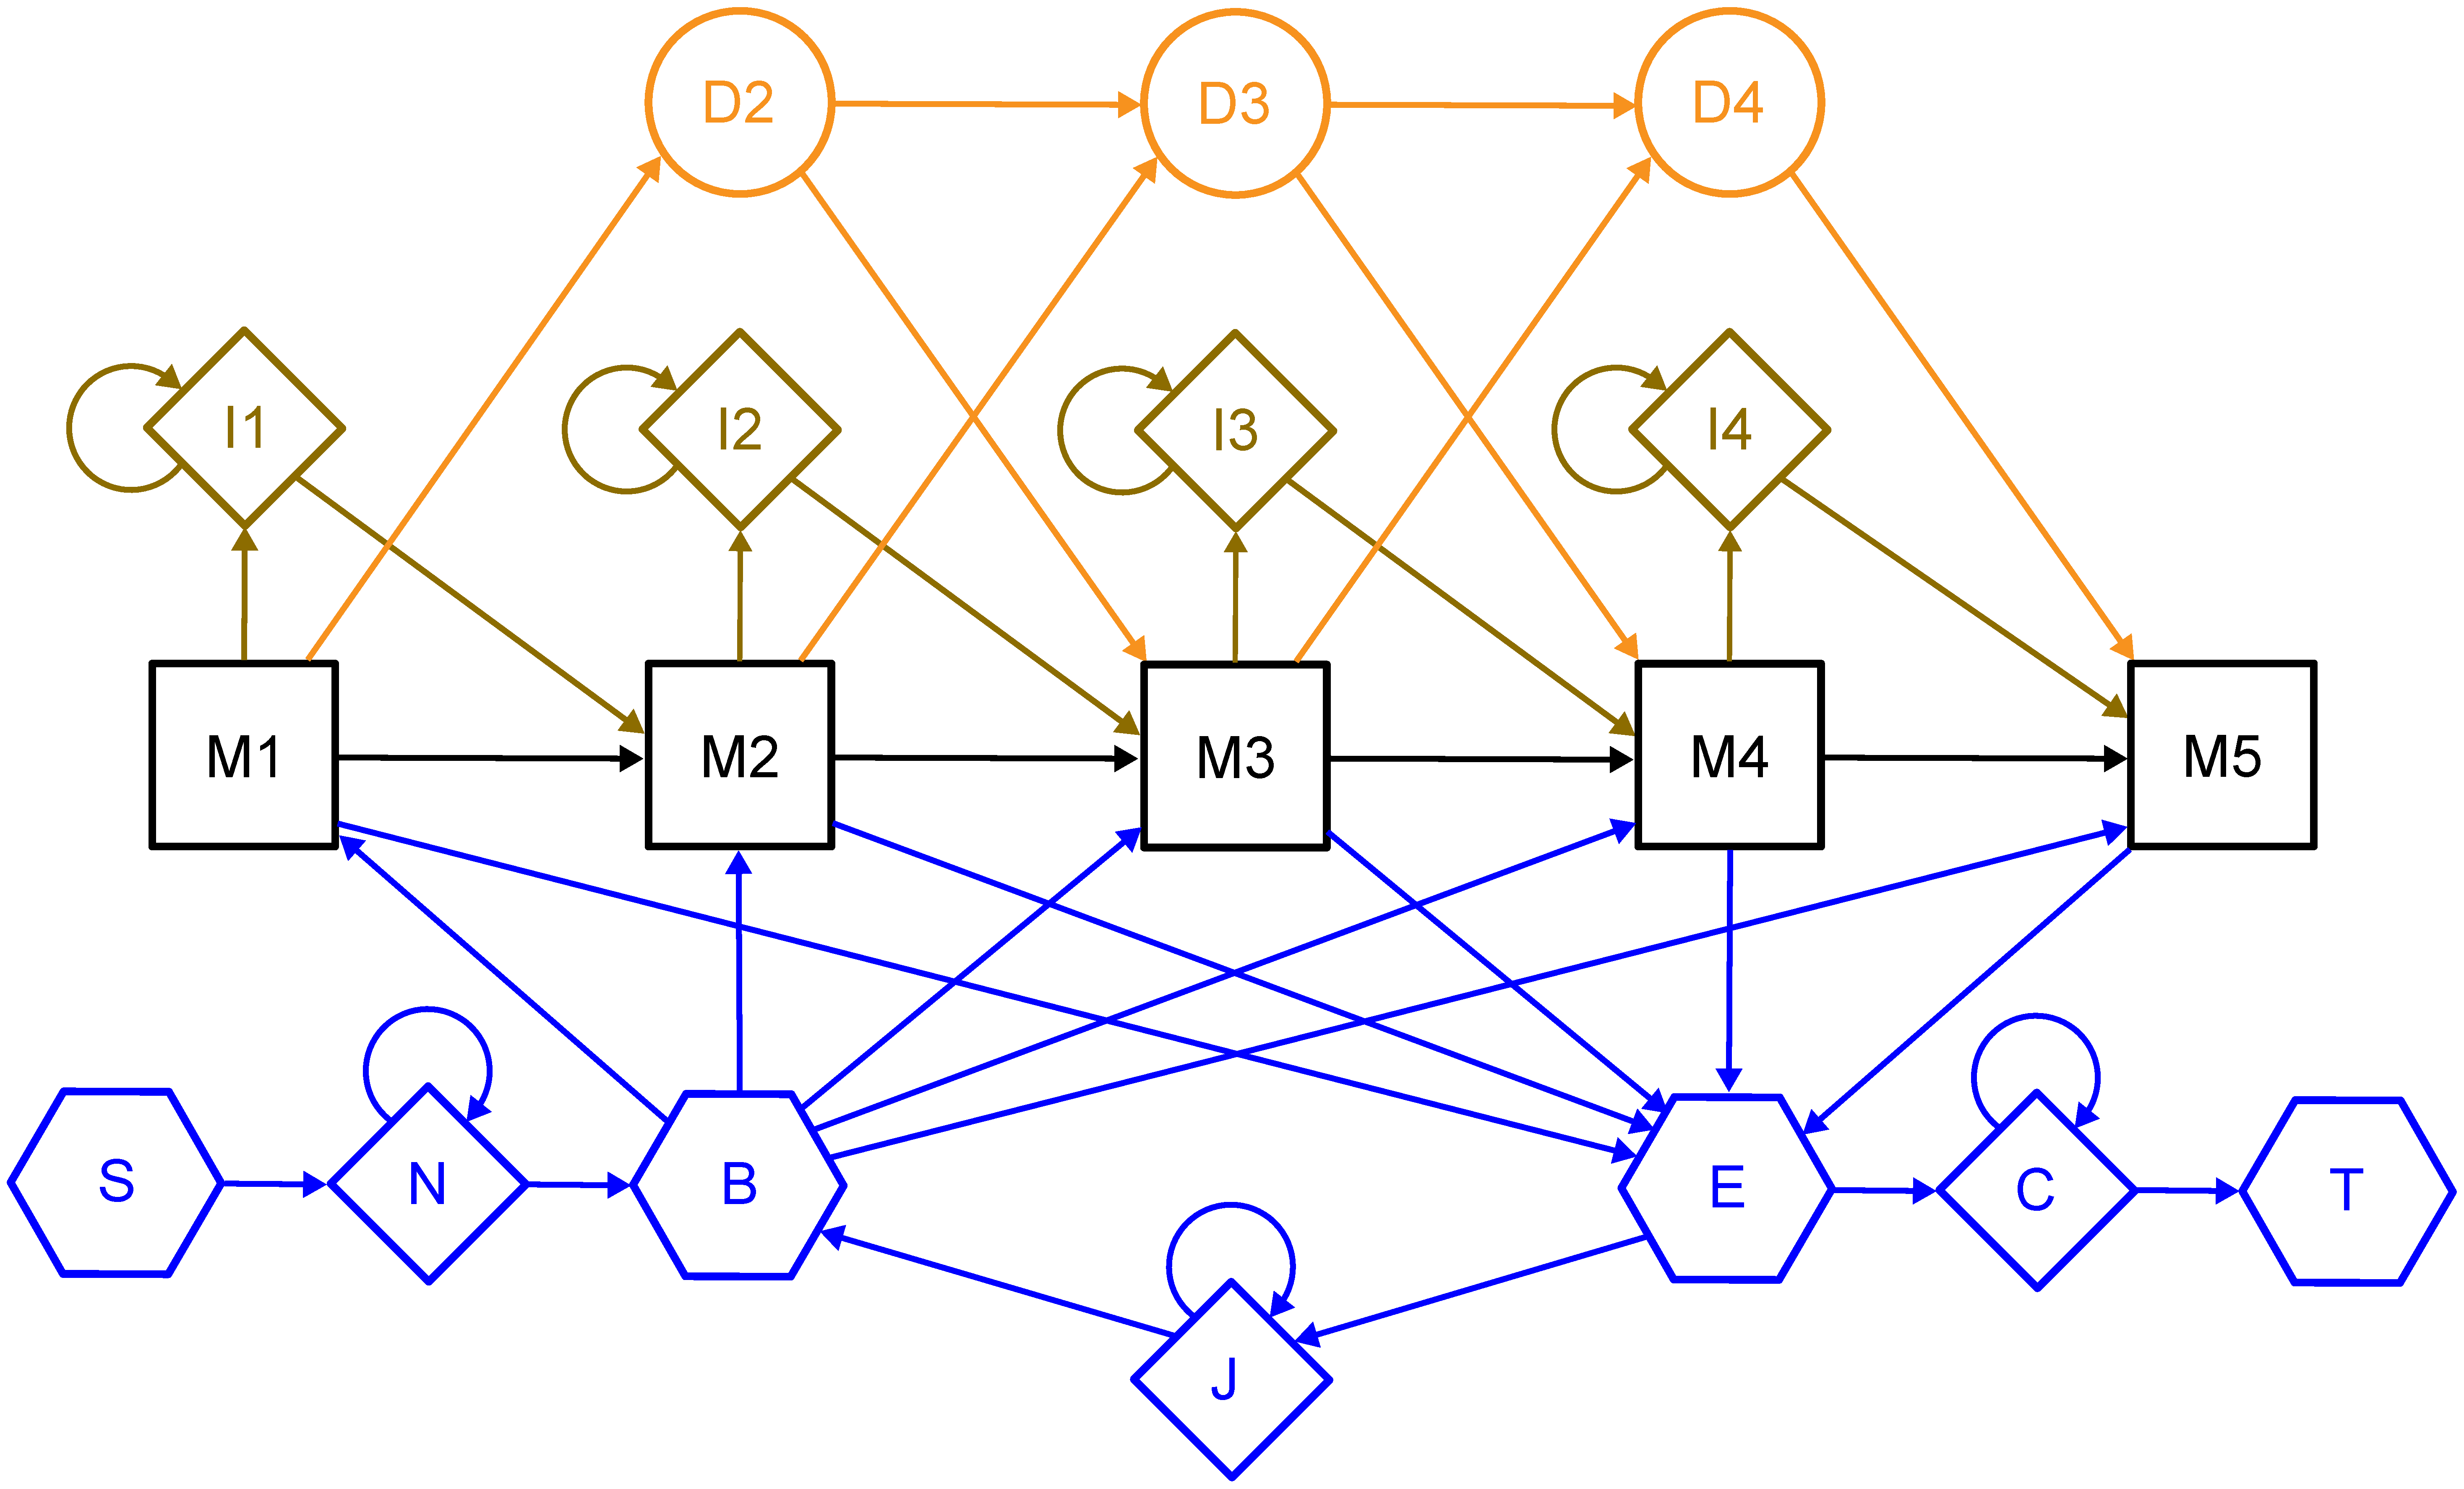
\includegraphics{img-hmm/hmmer-model.eps} }
    \caption[HMMER general model] {Complete model used by HMMER 3.0. Allows for multiple hits (multihit mode) in either local or global alignment mode. }
    \label{hmmer-model}
  \end{center}
\end{figure}

HMMER is a tool developed by Eddy \cite{eddy1998profile} that uses Hidden Markov Models to do sequence homology search. HMMER has become a very popular suite, and a strong focus of Profile \acp{HMM} research, with many efforts conducted to improve it and optimize it (\cite{hmmer-fpgas}, \cite{hmmer-gpus}, \cite{lindahl}, \cite{hmmer-mpi}, \cite{clawhmmer}).

The original version of HMMER relied on a model architecture similar to the Krogh-Haussler model, called 'Plan 9'(due to its nine transitions per state triplet). The current version employs the 'Plan 7' model architecture, shown in \autoref{hmmer-model}. The core of this architecture is similar to Krogh-Haussler/Plan 9, but Plan 7 has no D $\rightarrow$ I or I $\rightarrow$ D transitions, thus reducing the number of transitions to 7. Plus, Insert states have emission probabilities identical to the background distribution, canceling its component in the algorithm. 

Some special-states were also added to Plan 7 to allow for arbitrary restarts (thus making it a local alignment) and repeats (multihit alignment). These special states are parametrized to control the desired form of alignment (the HMMER \emph{alignment mode}). HMMER generally supports 6 different combinations of \emph{alignment modes}, formed by combining 2 options: unihit vs multihit alignments, and the basic alignment mode (global, glocal, and local). These are explained bellow: 

\begin{itemize}

\item Local mode: Aligns regions of the sequence against regions of the model. In unihit local alignment (HMMER's \emph{UNILOCAL}), only one region is matched. In multihit local alignment (HMMER's \emph{LOCAL}), multiple regions in the sequence and model are matched, and the same model region may be aligned multiple times (thus differing from classical Smith-Waterman);

\item Global mode: Aligns the whole sequence against the entire model. It corresponds to the Needleman-Wunsch algorithm. The special states self-looping states $N$, and $C$ are disabled, as well as the $B \rightarrow Mi's$ and $Mi's \rightarrow E$ transitions;

\item Glocal mode: The whole model is aligned against a subsequence of the target. This is an interesting particular alignment mode offered by HMMER. To make it work, the $B \rightarrow Mi's$ and $Mi's \rightarrow E$ transitions are disabled (thus forcing the whole alignment of the model) but the $N$ and $C$ self-looping states are enabled, to consume arbitrarily long  leading and trailing regions of the target sequence.

\end{itemize}

The original striped implementation of the Viterbi and Forward algorithms in HMMER used SSE units with 4 channels of (32 bit) floats. Floating-point values are the most suitable to the task, since we are dealing with probabilities with possibly many decimal places.

To increase the overall speedup, the data units were later changed to 8 channels of signed integer words (16 bit), through a discretization process of the floating-point probabilities. The discretization is done by a simple scaling operation, plus to an offset to gain a slightly larger representation space.

The SSE arithmetic uses signed saturation, which automatically limits overflowed values, that can then be checked for high-scoring hits. Underflows would be a problem however, since the algorithms use $-\infty$ scores as nullifying limit values, which should never touch the normal valid scores (i.e. scores without $-\infty$ terms). As such, HMMER uses a discretization range that ensures the normal scores will never underflow for model and sequence lengths below $10^{16}$ (\cite{hmmer3}).

The latest HMMER versions are HMMER 3.0, released in March 2010 \cite{hmmer3}, and HMMER 3.1b1 released recently in May 2013. 
Since HMMER 3.0, only the Local mode is supported in full; and, in particular, in the optimized implementations of the SSE-vectorized search filters. According to the author (\cite{hmmer-userguide}), accurate statistics are only available for the Local mode, and the other modes are poorly understood in terms of probabilistic significance. Furthermore, only the Local mode does not underflow the limited-precision presentation used in the SSE implementations.


\myparagraph{HMMER Pipeline}
\label{hmmer-pipeline}

HMMER 3.0 introduced a processing pipeline which uses a combination of incremental filters, each more accurate, restrictive and expensive than the previous one. \autoref{figure-hmmer-pipeline1} gives a representation of the filtering steps of the pipeline.

\begin{figure}[h!]
	\centering
	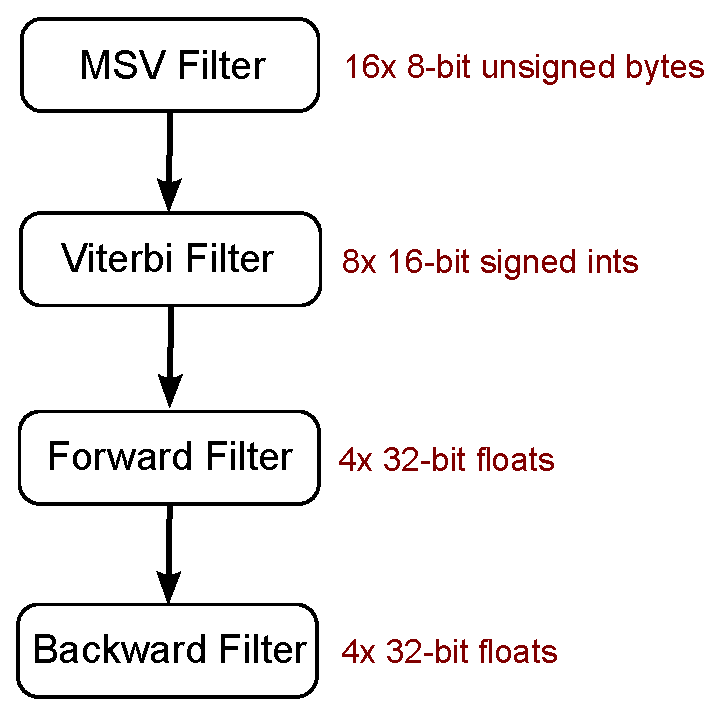
\includegraphics[scale=0.5]{img-hmm/hmmer-pipeline.eps}
	\caption{Diagram of HMMER's vectorized pipeline.}
	\label{figure-hmmer-pipeline1}
\end{figure}

The MSV (\emph{multiple segment Viterbi}) filter computes an optimal sum of multiple ungapped local alignment fragments. All of these filters have been parallelized with SSE, following Farrar's striped strategy, with increasingly higher precision. The fastest and coarser MSV filter uses 8-bit score values, the Viterbi Filter uses 16-bit scores, and the Forward and Backward filters use the full 32-bit floating point scores. In the case of Viterbi, an 8-bit precision was found to be insufficient and produce unacceptable high errors. The overall pipeline has also been parallelized to run on a multi-threaded, multi-node MPI environment with each thread processing each sequence independently.



%HMMER provides various different analysis tools, such as \emph{jackhammer} which performs an iterative database search, rebuilding and refining of the model after aligning each sequence to it, and \emph{hmmscan} which searches a target sequence against a database of profile models. On this work, the focus will be on \emph{hmmsearch}, the most used tool, that searches a target model against a sequence database.

%The application developed in this work, COPS, uses only Viterbi algorithm filter in unihit local mode (i.e., the mode more related to the original Smith-Waterman). 


%\cleardoublepage
\clearpage






%%%%%%%%%%%%%%%%%%%%%%%%%%%%%%%%%%%%%%%%%%%%%%%%%%%%%%%%%%%%%%%%%%%%%%%%%%%%%%%%%%%%%%%%%%%%%%%%%%%%%%%%%%%%%%%%%%%%%
%%%%%%%%%%%%%%%%%%%%%%%%%%%%%%%%%%%%%%%%%%%%%%%%%%%%%%%%%%%%%%%%%%%%%%%%%%%%%%%%%%%%%%%%%%%%%%%%%%%%%%%%%%%%%%%%%%%%%
%%%%%%%%%%%%%%%%%%%%%%%%%%%%%%%%%%%%%%%%%%%%%%%%%%%%%%%%%%%%%%%%%%%%%%%%%%%%%%%%%%%%%%%%%%%%%%%%%%%%%%%%%%%%%%%%%%%%%

\fancychapter{SIMD Inter-task parallel Viterbi}

\section{Proposed Solution}

The focus of the present work is to develop a parallelization approach based on SIMD (namely SSE on Intel Processors) inter-task vectorization for Profile \acp{HMM} algorithms. Rognes in 2011 (\cite{rognes2011}) pursued this strategy for alignment algorithms like Smith-Waterman. Building on Rognes' work, the same strategy can be followed for \acp{HMM} algorithms. 
However, as mentioned in the previous chapter, this is a promising new approach, that has not yet been much explored.
%this is still a rarely explored avenue which this work hopes to bring into more study. 

This work focuses on one of the most popular \acp{HMM} Homology search suites: HMMER \cite{hmmer3}. HMMER offers many tools, and one of the its key processing steps used by many of the tools is the Viterbi Decoding algorithm with a Profile \ac{HMM}. The Viterbi step is currently (as of May 2013) being implemented on SSE with Farrar's intra-task striped pattern. In this work, an alternative solution was developed, 
%Here, a new alternative solution was developed, that hopes to be competitive against, and improve on, HMMER's existing implementation. 

The Rognes-based implementation of Viterbi Decoding created in this work was named \emph{COPS} (Cache-Oblivious Parallel SIMD Viterbi). It is targeted at the HMMER suite and it is compatible with its internal configurations, being mostly interchangeable with the exception of the requirements of Inter-task parallelism (i.e. processing batches of sequences each time instead of just one). Also for this reason, COPS was developed on top of the HMMER suite as a standalone tool instead of being integrated into the HMMER pipeline of search filters (one of which being the Viterbi algorithm). A full integration into the HMMER pipeline was deemed unsuitable, since the pipeline is designed to process only one sequence at a time. Later work may extend this approach to the Forward algorithm as well and as into AVX2, Intel's new vector instruction set (an  extension of SSE).


%REVER ISTO
The following sections will present the developed implementation of the Viterbi algorithm with inter-task vectorization, the problems found, and two new methods to improve the strategy used by Rognes. Finally, the last section will describe a coarser-grained multi-threading parallelization of the algorithm itself, running on top the vector inter-task parallelization.





%%%%%%%%%%%%%%%%%%%%%%%%%%%%%%%%%%%%%%%%%%%%%%%%%%%%%%%%%%%%%%%%%%%%%%%%%%%%%%%%%%%%%%%%%%%%%%%%%%%%%%%%%%%%%%%%%%%%%
%%%%%%%%%%%%%%%%%%%%%%%%%%%%%%%%%%%%%%%%%%%%%%%%%%%%%%%%%%%%%%%%%%%%%%%%%%%%%%%%%%%%%%%%%%%%%%%%%%%%%%%%%%%%%%%%%%%%%


\section{Rognes-based SSE Inter-task vectorization}
\label{Rognes-based SSE Inter-task vectorization}

The main goal of this work consisted in implementing an inter-task vector parallelization of Viterbi Decoding in Intel's SSE, such as Rognes did for the Smith-Waterman algorithm \cite{rognes2011}.

Recall that this approach consists of using the N parallel SIMD channels for N different references (i.e. computing the Viterbi equations in parallel for the N sequences). This is known as 'Inter-task parallelism', as described previously in \sref{Inter-task Parallelism}. 

The initial implementation was largely based on Rognes' vectorization of the Smith-Waterman algorithm, with the changes necessary for the Viterbi problem. Since it is a form of inter-task parallelism, each channel is expected to perform the same operations, and thus the core of the algorithm maintains mostly the logic of the scalar version. The corresponding code  for the inner loop over the model states is presented in \cref{code-rognes}.

	
Initially, 32-bit floating-point values were used, which allowed for four independent channels in the SSE vectors. Four different sequences are fed into these four channels. Mmx, Imx and Dmx are the SSE dynamic programming arrays, respectively for Match, Delete and Insert state values. Mpv, Ipv and Dpv are auxiliary SSE registers to temporarily hold delayed or preempted values.
vB and vE are the SSE registers for the E and B flanking states values.

To compute the Match states, there are dependencies on M, D, and I, namely from the previous state triplet and previous sequence symbol (Mpv, Dpv, Ipv). These dependencies must be retrieved in the previous state iteration, \emph{before the writes}, to fetch the values of the previous symbol (indexes (i-1, k-1) in a \ac{DP} matrix) before they are re-written.
Each computed Match value is used to update the E (semi-end) state. 

In regards to Insert states, they depend on the M and I values in the same state-triplet, but from the previous sequence token. The M and I values can thus be fetched from the current state iteration, before the updates (saved in Mpv and Ipv).
Note that the D $\rightarrow$ I transitions have been removed by design from the model.

Finally, for the Delete states, there are D $\rightarrow$  D and M $\rightarrow$  D dependencies, from the same sequence token but previous state triplet (indexes (i,k-1)). To find these, it is necessary to preemptively compute and save the D and M values in the previous state iteration (Mnext saved and Dcv preemptively computed).

After each inner loop over the state triplets, the special states (E, J, C, N and B) are updated.


The measured performance (number of values computed per second) is mostly dependent on the model length (denoted by M, number of model state-triplets), with hardly any influence from the sequences length (denoted by L).
It achieved a 78\% performance improvement on the serial version by this initial parallelization with the Rognes-bases strategy. A diagram of the Rognes algorithm applied to HMMER is shown in \autoref{rognes-hmmer}.

\begin{figure}[htb!]
  \begin{center}
    \resizebox*{1.0\columnwidth}{!}{ 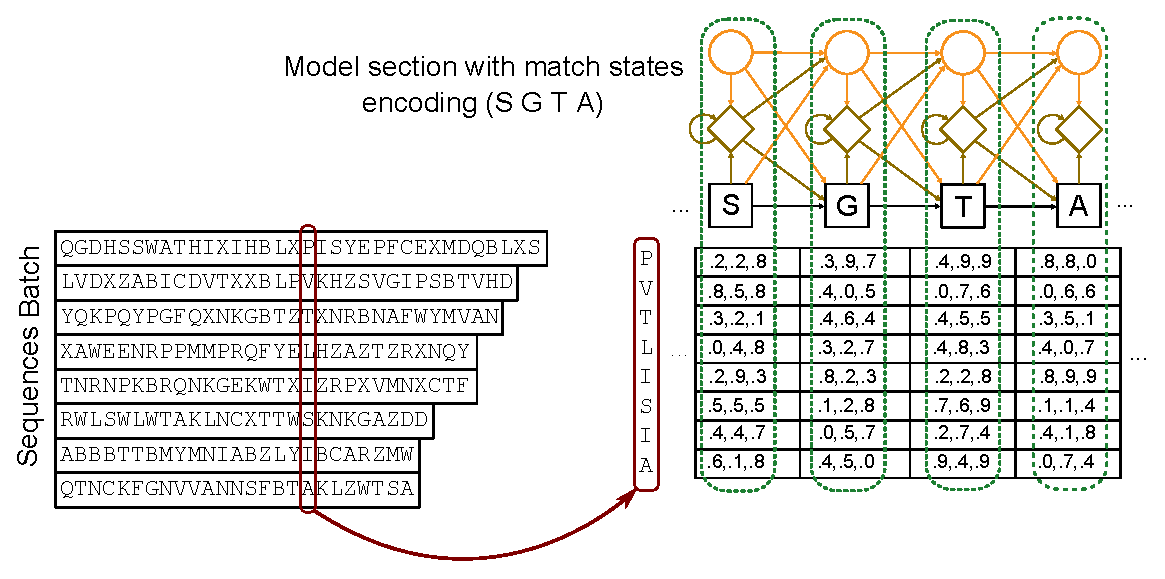
\includegraphics{img/rognes-hmmer.eps} }
    \caption[Vectorization of the Viterbi algorithm] {Rognes inter-sequence strategy applied to Viterbi Decoding in HMMER.}
    \label{rognes-hmmer}
  \end{center}
\end{figure}



\paragraph*{Initial Optimizations to the Rognes strategy}

\begin{itemize}

%The J transitions were removed from the model since our implementation does not support multihit alignments.
%Since our implementation only supports multihit local mode, the J state is disabled. As a result the E $\rightarrow$ C transition is always taken, hence the transition cost is 0 and can be removed from the algorithm.

\item Since the Insert emission scores are set to the background distribution in HMMER by default, they yield a null contribution and can be removed from the code.

\item It is possible is to pre-compute and save the $vB$ values for each state triplet. This however cannot be done when dealing with a dataset composed of varying-length sequences, since the model must be re-configured with each different sequence length.

\item For the main transition scores (i.e. between normal states), a single array was allocated, and the 8 transitions were stored in a interleaved manner, continuous in relation to the state triplets, in the order by which they are fetched in the inner loop. This allows for a better use of memory, avoiding mixed accesses to multiple different memory locations.
This arranged pre-allocated layout yielded a performance speedup of 15\%. 

\item Another improvement is unrolling the last iteration of the inner loop. The last iteration is particular since it only needs to compute the match value, hence the other operations can be removed.

\end{itemize}




\section {Loading of Emission Scores}
\label {Loading of Emission Scores}

Special concern was given to the method of loading and arranging the per-token Match Emission scores, because it was found that this step accounted for a substantial fraction of the overall time spent by the application. First the original method used by Rognes in the Swipe tool was implemented, evaluated, and then a new improved strategy was devised and implemented. The two are analyzed in the following sections.


\subsection{Rognes method of Loading the Emission Scores}

The Match Emission scores present a significant problem: it is impossible to arrange the emission scores in an memory-efficient pattern before the sequence tokens are known. A complete pre-arrangement of all possible $token \times state$ combinations would require $AlphabetSize^{AlphabetSize} \times L \times M$ 16-byte values. For DNA, which has an $AlphabetSize$ of 4, the required memory is manageable. For proteins, which are the usual target of such systems and have an usual $AlphabetSize$ of 21, it exceed the available memory of almost every system.The complete pre-calculation approach is infeasible.

To tackle this problem, initially, the loading of the Match emission scores was done using the method of Rognes' Swipe program \cite{rognes2011}. The method consists in pre-loading and arranging each quartet of emission scores ($4xM$, $M$ being the Model length), corresponding to the 4 parallel sequence tokens, necessary for the entire inner loop through the model states. For each new tuple of sequence tokens, an array of $M$ SSE vectors is computed and arranged for efficient access in the inner loop.

The costly arrangement must compute a transposition of the original scores, in successive rounds of 4x4 32-bit values: arrays indexed by symbol are transposed into consecutive tuples of 4 interleaved scores from the 4 different sequences. The transposition is achieved through SSE \emph{unpack} instructions, which interleave the lower or higher-order bits of 2 arguments, starting with a finer-grain unpack (32-bit unpacks when using 32-bit scores) and proceeding to coarser-grained unpacks (ultimately 64-bit unpacks that compute 128-bit values, size of the SSE vectors). This strategy is illustrated in \autoref{scores-loading-rognes}, with the corresponding pseudo-code shown in \cref{code-loading-rognes}.


\begin{figure}[htb!]
  \begin{center}
    \resizebox*{1.0\columnwidth}{!}{ 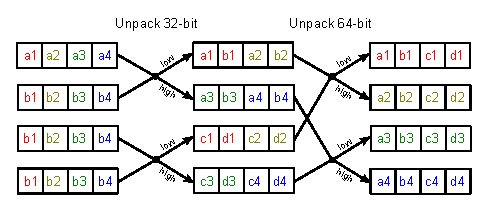
\includegraphics{img/scores-loading-rognes.eps} }
    \caption[Loading of Emission scores] {Emission scores pre-processing using SSE unpacks, according to Rognes' Swipe tool.}
    \label{scores-loading-rognes}
  \end{center}
\end{figure}


%\begin{algorithm}[htb!]
%\caption{ - Exemplo Listing }
%\label{code-listing-rognes}
%
%\lstset{language=C} 
%\begin{lstlisting}
%
%	/* Initialization of the zero row.	*/
%	xmxN = 0;
%	xmxE = xmxJ = xmxC = -eslINFINITY;			/* need seq to get here */
%	for (k = 0; k <= gm->M; k++)
%		dmx[k] = mmx[k] = imx[k] = -eslINFINITY;	/* need seq to get here */
%	/* DP recursion */
%	for (i = 1; i <= L; i++) 
%	{
%		float *rsc = gm->rsc[dsq[i]];
%		float sc, ipv, mpv, dpv, dcv;
%		dcv = mpv = dpv = ipv = sc = -eslINFINITY;
%		imx[0] = dmx[0] = mmx[0] = -eslINFINITY;
%		xmxE = -eslINFINITY;
%	}
%\end{lstlisting}
%\end{algorithm}

Besides the costly SSE operations in themselves, this method suffers from a poor memory utilization, requiring an additional write (and later read) to store and load the re-arranged scores. The results obtained point to roughly 30\% of the program runtime being spent in the arrangement of emission scores, a considerable amount.



\subsection{Inline method of Loading the Emission scores}

The original strategy for the pre-processing of emission scores, as developed by Rognes in Swipe, suffered from a serious performance penalty. In order to relieve this burden,  a new method was devised to keep Emission values as closer to the processor as possible, and thus avoid the drawback of the additional re-writing on memory. 

The transposition of scores is processed by rounds of 4 (since each SSE vector holds 4 floats, and the transposition must use a square 'matrix'), so the round of 4 values is the smallest block of data that can be transposed at the same time. The new method computes these 4-floats transpositions inlined between each round of 4 inner loop iterations. Each transposition produces 4 SSE vectors of emission scores, which can then immediately be used to compute 4 state triplets. The transposed scores are merely stored temporarily in close cache memory, and thus avoid the penalty hit of a full round of memory re-writings and improves the cache efficiency. This requires the inner loop be unrolled in 4 iterations.

After this transformation, the new inner loop consists of the code in \cref{code-loading-inline}. The optimization of interleaved scores' loading lead to an execution time roughly 30\% to 40\% faster than the pre-loading method used by Rognes' tool.

This method requires the number of model states to be a multiple of 4 (for 32-bit floats), to support the 4-state loop step. In order to easily deal with this, the model should be padded with dummy states up to a 4-state barrier. The dummy states carry dummy scores, set to $-infinity$, so that they have a null effect on the final results. These extra dummy states have a negligible effect on the overall performance.





\section{Discretization to 8x16-bit integer channels}

In order to increase the parallelization potential, the original 4 channel x 32-bit float version was converted to an 8channel x 16-bit integer version. This conversion implied a discretization of the floating-point scores, similar to the one employed by HMMER in its Viterbi Filter algorithm.

The discretization used a scale transformation with a factor configurable at compile-time. HMMER's authors estimate an optimal scaling factor of $\frac{500.0}{\ln 2}$, which does not underflow for any $L,M <= 10^{16}$ (\cite{hmmer3}).

Although 16-bit scores do not underflow (for any practical application), they may easily overflow when the sequence is slightly similar to the underlying family of the model. The occurrence of such overflows is detected by numerical manipulation of the vE values at the end of the inner loop.
%\begin{algorithmic}
%\LeftComment Select the overflowed channels
%\State newOverflows = \_mm\_cmpgt\_epi16(xmxE, vLimit)
%\LeftComment Union of the new overflowed channels with the older ones
%\State vOverflows = \_mm\_or\_si128(vOverflows, newOverflows)
%\end{algorithmic}


\myparagraph{3/2-nat optimization}
\label {3/2-nat optimization}

The 3/2-nat optimization was adopted to simplify the special-state calculations, and it is only valid for local alignment:
HMMMER assumes that, for local alignment with reasonable large and non-homologous sequences, only a small section will be matched. The rest of alignment will be merely filled with gaps (NN, CC, and JJ loops), totaling close to $L$ gaps. So, the optimization removes the NN, CC, and JJ loop transitions from the algorithm, and adds the correspondent cumulative sum of their contributions (3.0 for multihit mode and 2.0 for unihit) in the end. 

In COPS, it was equally applied the '-2.0 nat approximation' used by HMMER: N $\rightarrow$ N and C $\rightarrow$ C transitions are deleted, and a -2.0 offset bias is added to N in the beginning, and subtracted after the algorithm finishes. This value approximates the cumulative contribution of N $\rightarrow$ N and C $\rightarrow$ C insertion loops which, for a large $L$, is given by $ \log  \frac{L}{L+2}$.

%Eles substitutim estas transicoes por uma aprox para sequencias longas. No entanto o erro aumenta quando as sequencias sao semelhantes. 



\section{Model Partitioning to improve the L1 cache utilization}
\label{Model Partitioning to improve the L1 cache utilization}

A significant bottleneck was detected in the utilization of the innermost L1 data cache when using large models. This section will analyze the problem, and the solution that was found based on loop-tiling the inner loop.


\subsection{Problems with First-level Cache Efficiency}
\label{Problems with First-level Cache Efficiency}

At this point, early results showed a considerable performance degradation with an increasing Model length. After some experiments, it was found that the deterioration was caused by an exponential increase in the number of occurring L1 cache misses (the fastest cache level in Intel processors). It was also found that these L1D cache misses were overwhelmingly in the core inner loop of the code ($\sim$97\% of total cache misses).

An explanation for the explosion of cache misses seemed likely to be the eviction of the $M$-length auxiliary and scores' arrays from the cache between each execution of the inner-loop (i.e. between each outer-loop iteration). These arrays are re-used in each new passage through the inner loop, so it would be highly advantageous to keep the data in cache as long as possible. As such, a brief survey of the memory requirements of the most critical section of the code (the inner loop) is warranted. The original Rognes work likely did not suffer from these limitations, since the Smith-Waterman algorithm requires much less memory.

The estimated memory size of the data most heavily accessed by the inner loop is shown in \autoref{table-memory-comp}, for both HMMER's ViterbiFilter and this work's COPS.


\begin{table}[htb!]
\centering
\caption[Estimates of used inner loop memory] {Theoretical estimates of memory used by the core inner loop, in bytes}
\label{table-memory-comp}

\begin{tabular}{|c|c|c|}
\hline
	Spec & COPS, 16-bit integers   &   ViterbiFilter (HMMER), 16-bit integers   \\ \hline
	Mmx, Dmx, Imx	&	$3 \times M \times 1 6$	& $3 \times M \times 2$	\\ \hline
	Transition Scores	&	$8 \times M \times 16 $	& $8 \times M \times 2$	\\ \hline
	Match emission scores &	$M  \times 16 $		& $M \times 2$		\\ \hline
	Auxiliary Emission array &	$24 \times 16 $		&  \textendash		\\ \hline
	$\sim$20 aux. variables	&	$20 \times 16 $		& $20 \times 16 = 320$	\\ \hline
	Total			&	$192 \times M +700$	& $24 \times M  + 320$	\\ \hline
	Total minus E.M. scores &	$176 \times M + 700$	& $22 \times M + 320$	\\ \hline
	Max. $M$ to fill a 32KB cache &	$\frac{32768-700}{192} \approx 167 $	&  $\frac{32768-320}{22} \approx 1470 $ \\ \hline
\end{tabular}
\end{table}

We measured the computation performance and the number of L1D cache misses for the COPS tool of this work and the ViterbiFilter program of HMMER, using models of varying lengths. The performance was measured in million of state scores computed per second, using the Linux function \emph{ftime}. The cache profiling was conducted using Hardware counters, with the tool OProfile. \cite{oprofile} These tests were conducted on a commercial Intel Core2 architecture, with 32KB of the innermost L1D cache. The Emission match scores are only used once, they are never re-used, so their memory footprint and access pattern is an unavoidable hurdle, whose impact cannot be minimized.


The HMMER striped version uses a fraction of the memory requirements of COPS, mainly due to the shorter inner-loop and related vectors (with only $\sim$$\frac{M}{16}$ elements instead of $M$). This reduced memory footprint allows it to avoid the limits of the L1D cache for the inner-loop until a comfortably high model length (roughly 1470 in the estimates). The experimental results bear out this view (\autoref{cache-misses-nonpart}).

\begin{figure}[htb!]
	\centering
	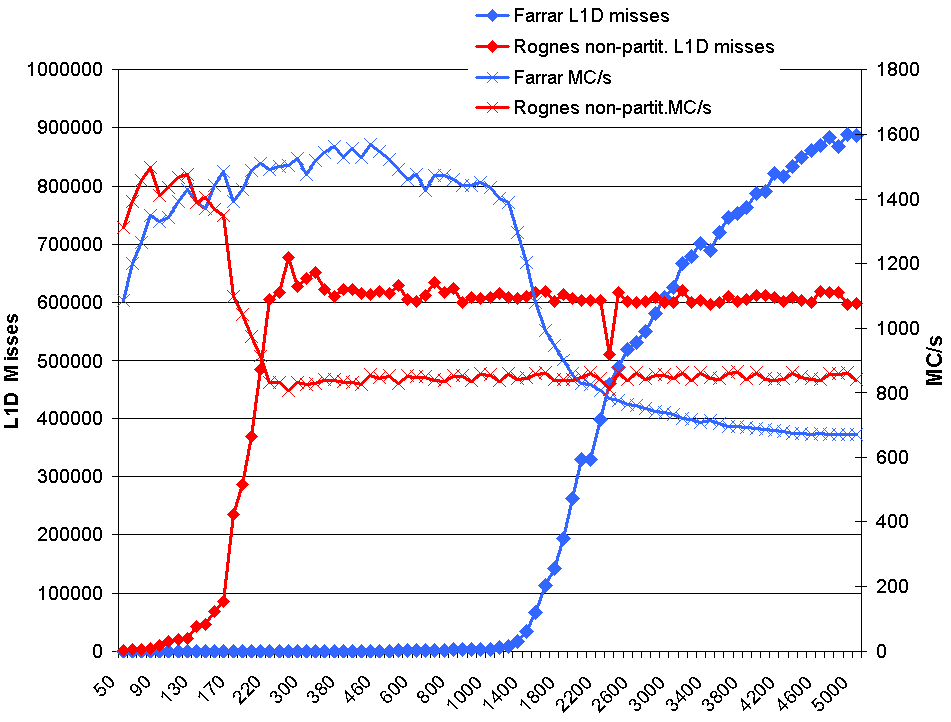
\includegraphics[width=16cm]{graphics/cache-misses-nonpart.png} 
	\caption[Cache profiling of non-partitioned models]  {Results of cache profiling of HMMER's Farrar-based ViterbiFilter, and the Rognes-based COPS, with a 32KB L1D cache. Measured in millions of cells computed per second (MC/s) and L1 data cache misses.}
	\label{cache-misses-nonpart}
\end{figure}

The theoretical estimates point to \emph{critical point} of full L1D utilization around $\sim$1470 for ViterbiFilter and $\sim$167 for COPS, for 32KB L1 data caches. These points coincide rather well with the observed spikes in cache misses and drops in performance, which figure strongly correlated in the results:

\begin{itemize}[noitemsep,nolistsep]

\item Rognes-based COPS: from a M of 120 to 220, there is a 26000\% increase in cache misses, and a 44\% drop in performance. Both the performance and the number of misses stabilize for M $>$ 220.

\item Farrar-based ViterbiFilter: between a M of 1200 and 2300, the number of misses rises 50000\% with the performance falling 43\%. Both the performance and the cache misses continue to deteriorate for longer models, although at a slower pace.

\end{itemize}

So, for practical applications, where the model length rarely exceeds 2000, COPS had a considerable memory handicap, which left it sorely uncompetitive vis-a-vis the striped ViterbiFilter. The graphic shows how the striped version was 70\% faster than the inter-sequence version for Ms between $\sim$180 and $\sim$1400. For models exceedingly long, starting with Ms $>$ 2400, COPS is again competitive and was able to achieve a small speedup against the HMMER implementation.





\subsection{Partitioning the Model}

In order to solve the cache efficiency problem, it was devised a \emph{loop-tiling} strategy based on a partitioning of the model states, that sought to limit the amount of memory required by the core loop. The normal model states are split in blocks of maximum \emph{M.P.} states, and the blocks are iterated over in a new outermost-loop. This corresponds to a standard \emph{loop-tiling} (a.k.a., \emph{strip-mining}) strategy, illustrated by the pseudo-code in \autoref{table-partitioning-comp}.

\begin{table}[htb!]
\centering
\caption[Inner loop code, before and after partitioning] {Comparison of the inner loop code, before and after partitioning the Model}
\label{table-partitioning-comp}

\begin{tabularx}{\textwidth}{ |X|X| }
\hline
Original code, non-partitioned  &  Strip-mined code, partitioned   \\ \hline

\begin{algorithmic}
\LeftComment Loop through the sequence symbols
\For {$i \gets 1 \textrm{ to } SequenceLength \ (L) $} 
	\State ...		

	\LeftComment Loop through the model state-triplets
	\For {$i \gets 0 \textrm{ to } M-1 $} 
		\LeftComment Core Viterbi code
		\State ...
	\EndFor
	
	\LeftComment Update the special states
	\State ...	
\EndFor
\end{algorithmic}

&
\begin{algorithmic}
\LeftComment  Loop through the partitions
\For {$i \gets 1 \textrm{ to } Npartitions $} 
	
	\LeftComment Loop through the sequence symbols
	\For {$i \gets 1 \textrm{ to } SequenceLength \ (L) $} 
	
		\State Load\_Data\_From\_Last\_Partition(i)
		\State ...		

		\LeftComment Loop through the state-triplets
		\LeftComment of the current partition

		\For {$i \gets 0 \textrm{ to } MP $} 
			\LeftComment Core Viterbi code
			\State ...
		\EndFor
	
		\LeftComment Update the special states
		\State ...	
		\State Store\_Data\_For\_Next\_Partition(i)
	\EndFor
	
\EndFor
\end{algorithmic}

\\ \hline
\end{tabularx}
\end{table}



The outer loop (new middle loop) over the sequences mostly re-uses the same memory locations (except for emission scores), which are accessed in the inner core loop, so these locations should be kept in close cache.
By limiting the model states loop to a maximum of \emph{MP} state-triplets, we can effectively guarantee that the whole sequence loop (the middle loop in the new layout) does not access more than roughly $\sim$ $(176 \times M + 320)$ bytes (disregarding the emission scores). The memory required by the inner loop is then cached in close memory, and repeatedly accessed over all the sequence loop while in cache, thereby reducing drastically the occurrence of cache misses.
The maximum partition length, \emph{MP}, is adjusted to achieve an optimal cache occupation, one that fills the available capacity of the closest data cache up to its limit.

There are two memory blocks which cannot be \emph{strip-mined} and thus degrade the performance of this optimization:

\begin {itemize}

\item Emission scores, which must be refreshed (re-computed) for each new round of sequence tokens. These values are only accessed once, so it is counter-productive to consider their cacheability.

\label{prefetching}
An attempt was made to prevent their loading into cache, by using the Intel \emph{software prefetch} instructions for non-temporal access, which tell the processor that the data is \emph{non-temporal} (i.e.; will never be reused) and thus should not evict other data from the cache. 
However, the non-temporal prefetches could not improve on the hardware prefetching already done by the processor, since the data access patterns are very regular (continuous actually). The number of LLC caches misses (i.e. for the larger L2 and L3 caches) is practically null.
% helper threads e prefetching n tem impacto

%An attempt to further exploit the parallelization potential of modern processors using Hyper-threading also proved infertile, actually yielding slightly slower code for Intel processors. In the case of AMD processors, the improvement from hyper-threading was very small. This shows how little time the program spends stalled, waiting for resources. 

\item Dependencies that must be exchanged between partitions. The last Match, Insert, and Delete contributions from each partition have to be carried on to the next partition, and so they have to be saved at the end of each partition. Each partition receives as input one line of previous states, with one state-triplet for each 8-fold round of sequences, and produces as output another line of values to the next partition. 

These dependencies can be minimized to 3 values per sequence round (vE, Mnext, and Dcv) after re-factoring the core code and moving the computation of Mnext with the 3 state dependencies to the end (\autoref{table-refactor-comp}).

\begin{table}[htb!]
\centering
\caption[Inner loop code, before and after refactoring the Match dependencies] {Comparison of the inner loop, before and after refactoring the Match computation to minimize the number of dependencies}
\label{table-refactor-comp}

\begin{tabularx}{\textwidth}{ |X|X| }
\hline

Original code	&  Refactored code \\ \hline

\begin{algorithmic}
	\LeftComment Loop through the model state-triplets
	\For {$i \gets 0 \textrm{ to } M-1 $} 

		\State $ Mnext \gets Max
					\begin{cases}
						vB + t_{BM}(k)	\\
						Mpv + t_{MM}(k)	\\
						Ipv  + t_{IM}(k)	\\
						Dpv + t_{DM}(k)	\\
					\end{cases} $ \\
		\State $ Mnext \gets Max(Mnext, e_{match}(k)) $

		\State $ vE \gets Max(vE, Mnext) $		
		\State $ Dpv \gets Dmx(k) $
		\State $ Ipv  \gets Imx(k)  $
		\State $ Mpv \gets Mmx(k) $
		\State $ Mmx(k) \gets Mnext $
		\State $ Dmx(k) \gets Dcv   $
		
		\State $ Imx(k) \gets Max
					\begin{cases}
						Mpv+  t_{MI}(k+1)	\\
						Ipv +  t_{II}(k+1)	\\
					\end{cases} $ \\

		\State $ Dcv \gets Max
					\begin{cases}
						Mnext +  t_{MD}(k+1)	\\
						Dcv +  t_{DD}(k+1)	\\
					\end{cases} $ 
	\EndFor
\end{algorithmic}
&
\begin{algorithmic}
	\LeftComment Loop through the model state-triplets
	\For {$i \gets 0 \textrm{ to } M-1 $} 

		\LeftComment Use partial value of Mnext
		\State $ Mnext \gets Max
					\begin{cases}
						Mnext \\						
						vB + t_{BM}(k)	\\
					\end{cases} $ \\
		\State $ Mnext \gets  Max(Mnext, e_{match}(k)) $

		\State $ vE \gets Max(vE, Mnext) $		
		\State $ Dpv \gets Dmx(k) $
		\State $ Ipv  \gets Imx(k)  $
		\State $ Mpv \gets Mmx(k) $
		\State $ Mmx(k) \gets Mnext $
		\State $ Dmx(k) \gets Dcv   $
		
		\State $ Imx(k) \gets Max
					\begin{cases}
						Mpv+  t_{MI}(k+1)	\\
						Ipv +  t_{II}(k+1)	\\
					\end{cases} $ \\
		\State $ Dcv \gets Max
					\begin{cases}
						Mnext +  t_{MD}(k+1)	\\
						Dcv +  t_{DD}(k+1)	\\
					\end{cases} $ 

		\LeftComment Partial computation of Mnext
		\State $ Mnext \gets  Max
					\begin{cases}
						Mpv + t_{MM}(k)	\\
						Ipv  + t_{IM}(k)	\\
						Dpv + t_{DM}(k)	\\
					\end{cases} $ \\
	\EndFor
\end{algorithmic}
\\ \hline
\end{tabularx}
\end{table}

\end {itemize}


\begin{figure}[htb!]
	\centering
	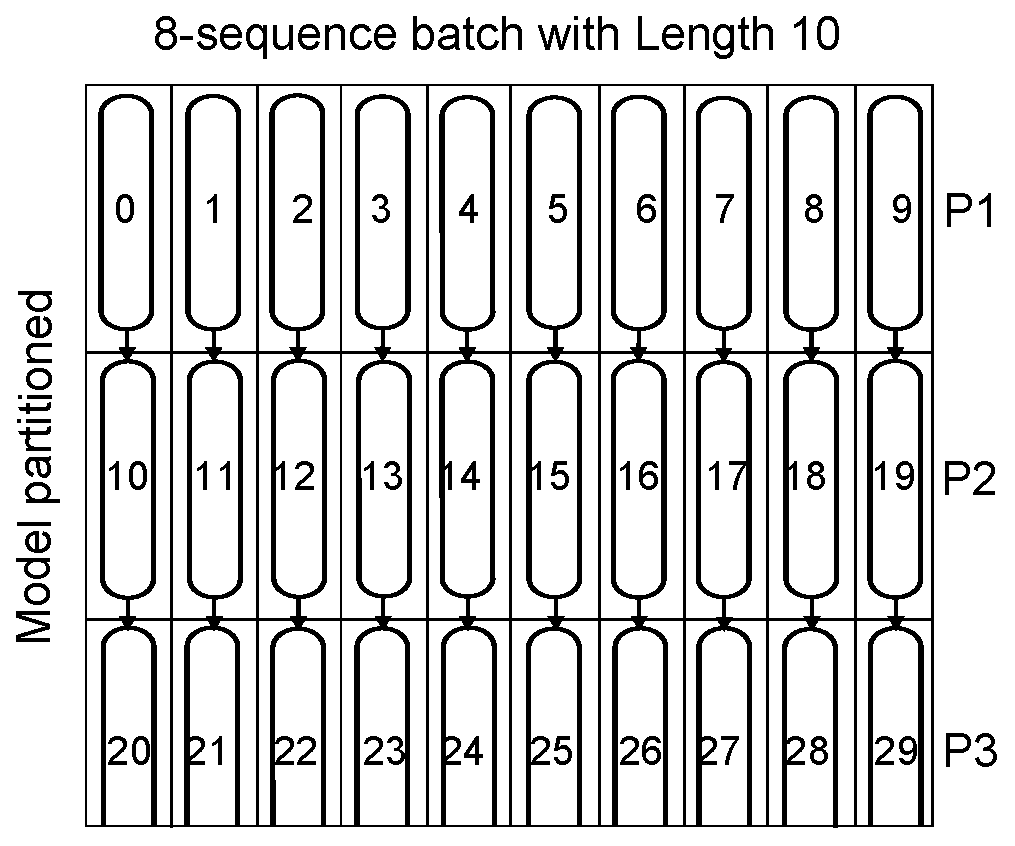
\includegraphics[scale=0.56]{img/partitions.eps} 
	\caption[Processing order in a partitioned model] {Processing pattern of the adopted partitioned model,with an 8-sequence batch of length 10. The numbers represent the processing order of each partition. The arrows show the inter-partition dependencies.}
	\label{figure-partitions}
\end{figure}

The processing order of the partitions is shown in \autoref{figure-partitions}.



\subsection{Problems of Model Partitioning}

There are some restrictions to the applicability of model partitioning however. The computation of each symbol-tuple through the model must be independent between each other. In particular, it must not depend on the final result of the previous symbol-tuple, which is the case for multihit alignments (alignment of the model multiple times against a sequence target). Therefore, the model can only be partitioned for unihit alignments (HMMER's 'uni-local mode'). In unihit alignments, the J special state, which encodes the token-to-token dependencies, is disabled.

The partitions used must necessarily have a length multiple of 8, to accommodate the loop step of 8 unrolled states. As a result, the model must be expanding up to a length also multiple of 8, by padding with dummy states and scores. The dummy scores are all set to -infinity so that they do not affect the result. The extra states add a slight performance penalty of extra computation.



\subsection{Determining the Optimal Empirical Partition Length}

Overall, the partitioned COPS implementation has an expected memory footprint of around $240*M + 900$ bytes (corresponding to the original memory requirements of the non-partitioned COPS, plus the additional arrays that are required to store the inter-partition dependencies). It can thereby be estimated the value for the maximum partition length ($MP$) as the maximum model length that limits the memory footprint to the size of the L1D. Hence the value of $MP$ can be determined by following the formula: $ MP = \frac{\displaystyle L1Dsize - 900}{\displaystyle 240} $.

Apart from a slight skew towards smaller lengths, justified by the sharing of the L1D cache with other variables not correlated with this processing loop, these estimated $MP$ values coincide very consistently with the best partition lengths that were experimentically observed:
\begin{itemize}[noitemsep,nolistsep]
\item 112 to 120 states, for 32KB L1D CPUs, (e.g. Intel Core, Core2, Nehalem, Sandy Bridge, Ivy Bridge and Haswell);
\item around 48  states, for 16KB L1D CPUs, (e.g. AMD's Opteron Bulldozer and Piledriver);
\item 216 to 224 states, for 64KB L1D CPUs, (e.g. AMD's Opteron K8, K10, Phenom I and II).
\end{itemize}

%These experimental values confirm the theoretical estimates of the L1D cache size limits, and its impact on inner loop data (see \autoref{table-memory-comp}).
%It was also observed that the size and policies of the outermost cache levels (usually L2 and L3 shared between cores) also affect the performance....
%Other processors will naturally have a different optimal value, mainly depending on the cache architecture (levels, policies and sizes of caches).



\subsection{Evaluation after Partitioning}

After partitioning, the overall performance behaved remarkably as expected, maintaining the same level of caches misses and computation speed for any model length:

\begin{figure}[h!]
	\centering
	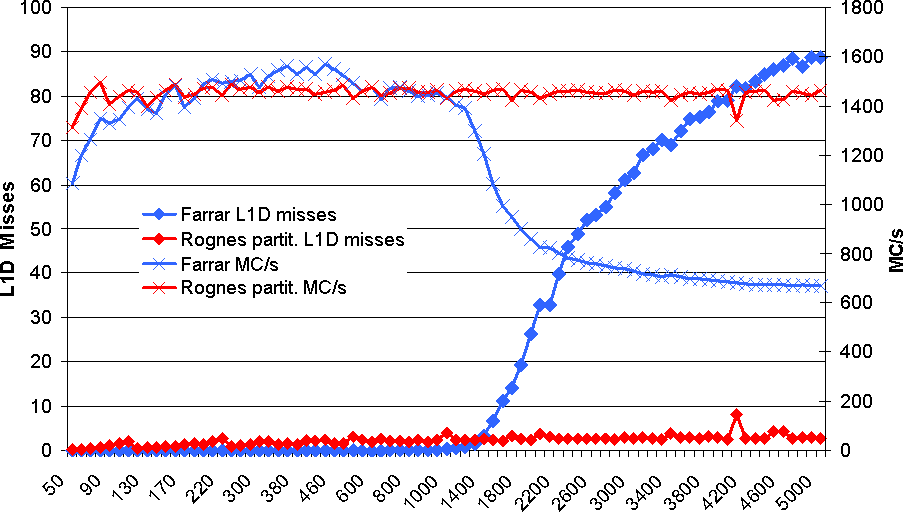
\includegraphics[width=16cm]{graphics/cache-misses-part.png} 
	\caption[Partitioning performance results] {Results of cache profiling of HMMER's Farrar-based ViterbiFilter, and the new partitioned COPS. Measured in millions of cells computed per second (MC/s) and L1 data cache misses.}
	\label{cache-misses-part}
\end{figure}

As a result, COPS managed to be slightly faster than HMMER's ViterbiFilter for models up to $\sim$1200, after which the COPS program quickly gains a close to 2-fold speedup over ViterbiFilter, due to the latter's cache degradation.

Compared to the non-partitioned COPS code, the partitioned version was about 42\% faster for long models ($\sim$1000) \emph{before refactoring the inner loop code}. After refactoring the auxiliary storage arrays (Mpv, Ipv, Dpv), the improvement was of 49\%. The complete pseudo-code of this final version is presented in \cref{code-complete} and \cref{code-compute}.




\section{Batches of Sequences with varying lengths}

Since the program runs with 8 parallel sequences in lock-step, there is a problem when the sequences have different lengths. The program must then either ignore the shorter sequences and continue until all sequences are completed (the static approach), or feed in new sequences to replace the finished ones, while the algorithm is running (the dynamic approach used by Rognes). 

The two possible approaches were implemented in this work, and their performance compared:

\begin{itemize}

\item \textbf{ Static approach: restarting the execution every time to load new sequences }
%\paragraph{Static approach: restarting the execution every time to load new sequences}

The sequences are padded with dummy valid symbols (e.g.; any residue) up to the length of the longest sequences, for each new group of sequences processed. The dummy residue maps to a score array of $-\infty$ scores. These emission scores cancel the updates of vE by the Match states $M$ when they are added to the computation of $M$.

In the 32-bit floating point implementation, additional concerns are required: the C $\rightarrow$ C transition cannot be eliminated with dummy scores. It was necessary to mark where each sequence terminates (i.e. its length), compare the limit length in each iteration, and then, by numeric manipulation, nullify the C $\rightarrow$ C transition for iterations beyond the limit length.

The wasted computation incurred by the dummy symbols was evaluated with a practical-use database (NRDB90) and found to be minimal: it accounted for less than 0.01\% of the total computing effort.
% Besides this penalty of redundant computation, there are additional drawbacks to this approach. Estao no texto abaixo do itemize


\item \textbf{ Dynamic approach: runtime swapping of sequences }
% \paragraph{Dynamic approach: runtime swapping of sequences}

The Dynamic swapping method was chosen by Rognes for his Swipe tool. In this approach, the sequences are checked in each iteration of the outer loop (loop over sequence symbols) to determine if any has reached its end. Those that have, are exchanged with the next database sequence, and the appropriate SSE vector elements in the auxiliary data arrays are reset to $-\infty$.

\end{itemize}


The performance of both methods was evaluated with both a randomized dataset of multiple-length sequences, and the NRDB90, whose sequences have more disparate lengths. On both tests, the Static approach proved to be about $\sim$60\% faster than the dynamic approach.

Furthermore, the Rognes dynamic method has a few limitations, which inhibits its use in the present work:

\begin{itemize}[noitemsep,nolistsep]
\item The sequence loop must be the outer-most loop, and by consequence it would not be possible to employ the Model partitioning optimization.
\item The parametrization of the model targeted to each particular sequence Length would equally prove impossible to conduct, since the entire database must be evaluated in a single execution run, without the possibility of re-starts and re-parameterizations.
\end{itemize}

Even if the swapping method were more efficient, these two limitations are enough to seal the decision of instead using the re-starting method in COPS.

However, with the static re-starting method, there is also an additional source of non-negligible scoring errors in the mis-parametrization of the sequences in the group. Before each execution of the algorithm, the model is reconfigured with the average sequence Length value among the 8 sequences. In particular, the re-configuration computes the transition scores of the special states. Since 8 sequences are processed in lock-step, if their lengths differ, the shorter sequences will yield slightly biased scores. This error can be minimized by first sorting the database sequences, which for practical large databases results in an uniform length for most 8-sequence batches. The re-configuration of the model is a very short step, and does not cause any measurable performance penalty.

The sorting step was done by the standard C implementation of the Quicksort algorithm. Its runtime cost was measured, and determined to be negligble in the context of the application. It took less than 0.01\% of the overall runtime, even when sorting large databases with either many small sequences, or fewer but larger sequences.





\section{Multi-threading the partitions}
\label{Multi-threading the partitions}

After having a partitioned model, each partition can be seen as a 'chunk' of data to process. This data layout seems particularly suitable for an additional level of paralellization: multi-threading using a wave-front model of partitioned chunks. From the start, the parallel speedup over the number of threads would expectedly never reach linear growth (mainly due to the unavoidable synchronization and communication between threads). Still, this second parallelization level is an interesting improvement, which could be applied to other areas (e.g.; single tasks that cannot be linearly decomposed into independent threads).


With a partitioned model, it is possible to add \ac{SMP} multi-threading to parallelize the partitioned chunks. Some number, $N$, of partitions are simultaneously processed by $N$ threads, following a wave-front pattern: each thread starts its assigned partition of the $i$-th sequence residue when the previous thread has finished the previous partition of the same $i$-th sequence residue (\autoref{wave-front-model}). The computing pattern is thus 1) left-to-right (ascending by sequence index), and 2) top-to-down (ascending by model state index).

\begin{wrapfigure}{r}{0.3\linewidth}
%    \resizebox*{0.3\columnwidth}{!}{ \includegraphics{img-hmm/wave-front-model.eps} }
	\includegraphics[width=1.0\linewidth]{img-par/wave-front-model.eps}
	\caption[Multi-threaded Wave-front pattern] {Multi-threaded Wave-front pattern. Blocks are processed concurrently in a diagonal pattern (same color for concurrent partitions). }
	\label{wave-front-model}
\end{wrapfigure}

The main-master thread has some special tasks that distinguish it from the worker-slave threads: it is the only thread responsible for loading the sequences, resetting the control and synchronization flags, and re-configuring the model.

There are two synchronization concerns involved in the multi-threaded wave-front strategy: synchronization of all threads at the start of the algorithm (since it is run multiple times using the same $N$ threads), and synchronization of data between threads processing inter-dependent chunks. These two concerns will be explained in detail in the following subsections.


\subsection{Execution call synchronization}

The first level of synchronization concerns the sequentiality of calls to the algorithm, each call running with the same threadpool, requiring synchronization of all threads before starting each new execution of the algorithm. The synchronization here is essential to allow time for the main thread to do its preparation work between runs. On the other hand, it is desirable that the synchronization be as efficient and lightweight as possible.

A few methods were tried, which either did not ensure the proper synchronization, or were not optimally efficient:

\begin{itemize}

%\item Mutexs and signals
%
%\begin{algorithm}[htb!]
%\caption{ - Pseudo-code of synchronization method with mutexes and signals}
%\label{code-mutexs}
%
%\begin{algorithmic}
%\State MutexLock(synchMutex)
%\If{MASTER}
%	\State ConditionBroadcast(synchCond)
%\Else 
%	\State ConditionWait(synchCond, synchMutex)
%\EndIf
%\State MutexUnlock(synchMutex)
%\end{algorithmic}
%\end{algorithm}
%
%This method fails because it requires the main thread to be the last entering the mutex, which usually happens, but it's not guaranteed.


\item Synchronization barrier from Pthreads library

This approach consists of the primitive pthread\_barrier from the POSIX Pthread library, which acts on a 'barrier' variable initialized with the desired number of threads. When the method 'Wait' is called by a thread, it is blocked by in the barrier until all threads have called the same method. 
This primitive achieves the synchronization requirement of this project, but it is slower than other methods.


\item Per-thread semaphores

\begin{algorithm}[htb!]
\caption{Pseudo-code of synchronization method with Semaphores}
\label{code-semaphores}

\begin{algorithmic}
	\LeftComment Declaration:
	\State Semaphore synchSems[NTHREADS]
		
	\LeftComment Initialization:
	\For{$i \gets 0 \textrm{ to } Nthreads $} 
		\State SemaphoreInit(synchSems[i], 0)
	\EndFor
	
	\LeftComment Worker:
	\State SemaphoreWait(synchSemaphores[myThreadId])
	
	\LeftComment Main:
	\For{$i \gets 0 \textrm{ to } Nthreads $} 
		\State SemaphorePost(synchSemaphores[i])
	\EndFor
\end{algorithmic}
\end{algorithm}


The semaphores are initialized with a value o 0. To start each run, the main thread signals each worker thread that it can start, using the \emph{Post} method. Each worker thread calls the \emph{Wait} method on its corresponding semaphore. This method will either block and wait if the main thread hadn't signaled it yet, or consume one value and proceed if otherwise. The workers that are waiting on the semaphores are woken up by the main thread signals.

The semaphores technique works but it is again slower than other methods.



\item Per-thread start flags

This method uses an array of simple synchronization flags (integers), one per thread, wherein each thread may wait for a command from the main thread.

\begin{algorithm}[htb!]
\caption{Pseudo-code of synchronization method with Per-thread start flags}
\label{code-startflags}

\begin{algorithmic}
	\LeftComment Worker:
	\While { syncFlags[myThreadId] is False }
		\State YieldCPU()
	\EndWhile
	\LeftComment after leaving the loop, and seeing a True flag, reset it to False:
	\State syncFlags[myThreadId] = False

	\LeftComment Main:
	\For{$i \gets 0 \textrm{ to } Nthreads $} 
		\State syncFlags[i] = True
	\EndFor
\end{algorithmic}
\end{algorithm}

Again, this is a functional and lightweight method, but it was deferred in exchange for a more slightly better approach.

\end{itemize}

In the end, the chosen method was a variation of the Per-thread start flags, that uses a single global execution counter and per-thread local counters:

\begin{algorithm}[htb!]
\caption{Pseudo-code of synchronization method with Per-thread local counters}
\label{code-counters}

\begin{algorithmic}
	\LeftComment Main:
	\State Inc globalExecCounter

	\LeftComment Worker:
	\State myExecCounter = 0
	\While { True }
		\State Inc myExecCounter
		\While { globalExecCounter $\neq$  myExecCounter }
			\State	YieldCPU()
		\EndWhile
		\State Call DoWork()
	\EndWhile

\end{algorithmic}
\end{algorithm}


The worker waits (yielding the CPU) until its local replica counter matches the value of the global counter, whose value is only set by the main thread.
There are no data consistency concerns here, simply because outdated values of the global counter will not cause undesired behavior, such as workers' early starts. The only problematic effect of out-of-date values is possibly additional wait cycles for the workers.

Two simple benchmarks were used to evaluate the relative performance of each synchronization method: a first benchmark (\autoref{synch-computation}) consisting of a small model and small generated random sequences ($\sim$100 residues each); and a second benchmark (\autoref{synch-nocomputation}) that stressed the synchronization primitives alone, with no computation whatsoever.

\begin{figure}[htb!]
    \begin{minipage}{0.48\linewidth}
		\centering
		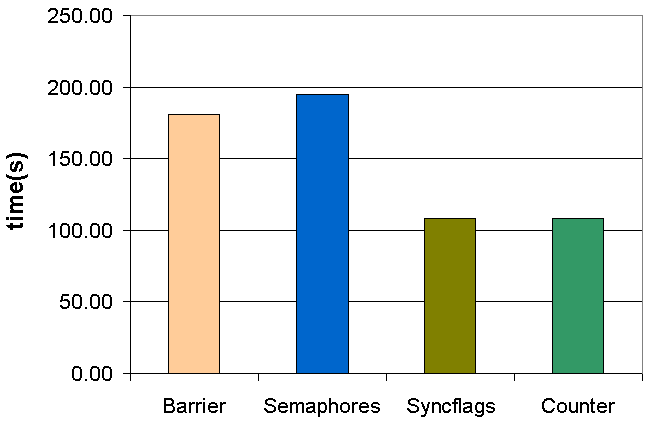
\includegraphics[width=7.5cm]{graphics/synch-computation.png} 
		\caption[Synchronization Evaluation with computation] {First benchmark: COPS code with a 100-length model, 4 threads, and 800K 100-length sequences.}
		\label{synch-computation}
    \end{minipage}
    \hspace{0.04\linewidth}
    \begin{minipage}{0.48\linewidth}
		\centering
		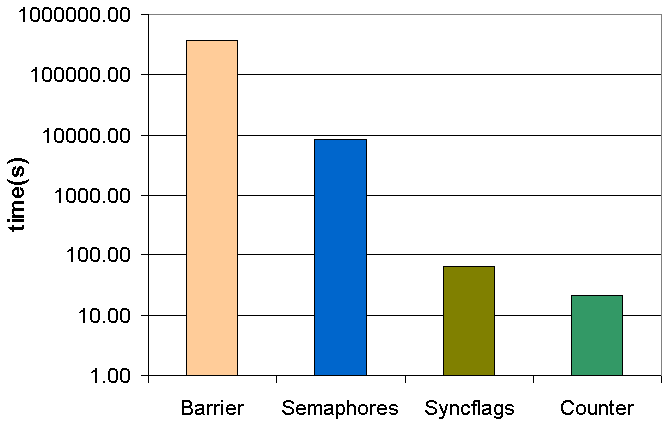
\includegraphics[width=7.5cm]{graphics/synch-nocomputation.png} 
		\caption[Synchronization Evaluation without computation] {Second benchmark: only synchronization primitives, in $80K \times 80K$ rounds. Logarithmic scale.}
		\label{synch-nocomputation}
    \end{minipage}
%	\caption{Relative performance of the various synchronization methods. Tested on a quadcore Intel Core2duo.}
\end{figure}


These results show that the Counter method is indeed the most efficient solution. Note the logarithmic scale on the second benchmark, clearly illustrating the disproportionate efficiency of the no-locks methods vis-a-vis the locking approaches.

Finally, it was evaluated the overall percentage of idle thread time incurred by the chosen method (global Counter + local counters). A battery of tests was run, starting from sequences with a large amount of wasted computation lines due to partitioning, and down to sequences with no wasted computation. The determined result was that the total idle thread, cumulative of the 4 threads used, ranged from < 1\% to a maximum of 5\% in the worst case, with an average between 0\% and 2\%. These values are reasonable and quite positive for the average case.


	
\subsection{Partition synchronization}

The second level of synchronization concerns the exchange of data between threads processing adjacent partitions. Namely, each thread must send data to the thread processing the succeeding partition, independently for each sequence index. Moreover, each thread must block itself while it is waiting for data from the preceding partition, and this procedure repeats for each and every sequence index. The synchronization overhead is reduced by the decomposition by sequences indices, resulting in relatively small work-chunks of size $PartitionLength \times 1$.

To implement this synchronization requirement, it was chosen a simple and efficient solution: 
\begin{itemize}
\item $Nthreads$ arrays of flags, one for every pair (partition, sequence symbol), wherein threads can wait and signal one another. The wait is implemented by yielding the CPU and the signaling is done by setting the flag.

\item Unique arrays (with length equal to the sequence length) for the data that needs to be exchanged.
Only one array is needed for each type of data, because only one transfer of data can occur at any given time for each sequence symbol (i.e.; the data is propagated only one thread at a time, every time the active thread finishes and passes its data to the next partition thread). Only one thread is active processing a sequence index at a given time, any other thread is either in a previous index or waiting on the preceding partition thread.
\end{itemize}

The chosen synchronization technique has the precious benefit of not using any locks or blocking primitives.
No memory barriers are needed, because stale data is not a problem for the program. Data that is not updated will cause no consistency problems, rather it will merely lead to more waiting (yielding) cycles. The flags are only reset by the master thread, before starting the algorithm.

%Volatiles parece que tambem nao sao precisos. Mas nao tem impacto na performance.
	

\subsection{Computing the Practical Threaded Partition Length}

A relevant issue to consider is what partition length should be used in each case? This practical partition length differs from the theoretical optimal length by taking into account the computation effort that is wasted by idle threads when the partitions are not evenly divisible by the threads.

The optimal length depends on a few variables: model size, number of threads, and optimal partition length (which is used as a maximum threshold for the practical length), with the stated goal of finding a partition length that maximizes the effective thread use.

\begin{enumerate}

\item It is computed the number of minimum (i.e. assuming the threshold length) total chunks required to cover the complete model, and that are a multiple of the number of threads:
	$MinNchunks = roundtop(\frac{M}{MaxPartLength}, Nthreads)$

\item This minimum number of chunks is used to compute the practical partition length (which has to be a multiple of the SSE vector size, 8):
	$ PartitionLength = roundtop(\frac{M}{MinNchunks}, 8) $

\item The actual number of partitions is finally calculated based on the partition length chosen:
	$Npartitions = ceiling(\frac{M}{PartitionLength} ) $
	
\end{enumerate}

% AQUI podia-se falar do calculo do trabalho desperdicado

The partitions are then issued to the available threads, using static decomposition and a fixed pinning scheme that ensures the last partition belongs to the master thread (which has the last ThreadId). This is important because it is the master that deals with the algorithm terminations, and extracts and computes the final result.

The following formula was used to determine the start partition of each thread:
	$StartPartition = (Npartitions + myThreadId) \mod Nthreads $

	


%\cleardoublepage
\clearpage

		


	
	


%%%%%%%%%%%%%%%%%%%%%%%%%%%%%%%%%%%%%%%%%%%%%%%%%%%%%%%%%%%%%%%%%%%%%%%%%%%%%%%%%%%%%%%%%%%%%%%%%%%%%%%%%
%%%%%%%%%%%%%%%%%%%%%%%%%%%%%%%%%%%%%%%%%%%%%%%%%%%%%%%%%%%%%%%%%%%%%%%%%%%%%%%%%%%%%%%%%%%%%%%%%%%%%%%%%

\fancychapter{Evaluation}

In this chapter, it will be evaluated the performance gain from each of the main contributions of this work, culminating with the complete multi-threaded version. The results obtained from each benchmark against the relevant comparable software, HMMER's Farrar-based ViterbiFilter vectorization, will be presented and discussed.

\section{Evaluation Methodology}

This section will describe the evaluation methodology and configuration used for the various tests, as well as the features being evaluated. 

\subsection{Benchmark implementations}

As previously described in \sref{hmmer-pipeline}, HMMER uses a multi-level processing pipeline to conduct most sequence homology search tasks. This pipeline is composed by a few filtering levels, each more expensive and fine-grained than the previous one. The current pipeline (HMMER version 3.1b1) has the structure presented earlier in \autoref{figure-hmmer-pipeline1}.

The COPS implementation developed in this thesis targets the second level, as an improvement on the Viterbi Decoding filter of the pipeline. However, the whole pipeline processes the sequences sequentially, one by one, and not in parallel. The multi-threaded parallelization of in HMMER is done by running one different pipeline in each thread. The pipeline itself supports only one thread processing a single sequence.
This pipeline architecture is thus incompatible with both the Rognes method (inter-task vectorization of N concurrent sequences) and the multi-threading developed in COPS (threading of partitions in a wave-front decomposition). 

Given this incompatibility, it was impossible to integrate the developed COPS code into the HMMER pipeline. Instead, the code was packaged into a small stand-alone tool, built on top the HMMER suite. It uses the HMMER libraries and models, and serves as a proof-of-concept for the developed techniques and architecture.

In order to evaluate the overall performance of COPS vis-a-vis the HMMER Viterbi Decoding implementation (i.e., the ViterbiFilter program), a small multi-threaded test tool was created for ViterbiFilter. The benchmark runs with multiple-threads to be fully comparable to the multi-threaded COPS. The used threadpool was implemented efficiently with mutexes and a single synchronized sequence counter.

Besides HMMER's ViterbiFilter, the benchmarks were also run against a serial implementation of Viterbi, optimized for the alignment mode used (Unihit Local alignment).



\subsection{Evaluation Dataset}

To evaluate the developed application, an extensive and thorough range of benchmarks was carried out. The evaluation dataset consists of:

\begin{itemize}

\item HMMs sampled from the Dfam database of Homo Sapiens DNA (\cite{pfam}), with model lengths from 60 to 3000, increasing by a step of roughly 100 model states each time.

Dfam is a widely used database of protein families, and \acp{HMM}s constructed to model them. The latest release of Dfam, as of March 2013, uses HMMER3.1b1 to create the Hidden Markov models. The complete list of chosen HMMs from Dfam is presented below (their length is prefixed to the model name): 

\vspace{1px}
\begin{tabular}{llll}
M0063-U7		& M0700-MER77B			& M1409-MLT1H-int	& M2204-CR1\_Mam	\\
M0101-HY3		& M0804-LTR1E			& M1509-LTR104\_Mam	& M2334-L1M2c\_5end	\\
M0200-MER107	& M0900-MER4D1			& M1597-Tigger6b	& M2434-L1MCa\_5end	\\
M0301-Eulor9A	& M1000-L1MEg2\_5end	& M1727-L1P3\_5end	& M2532-L1MC3\_3end	\\
M0401-MER121	& M1106-L1MD2\_3end		& M1817-REP522		& M2629-L1MC4a\_3end\\
M0500-LTR72B	& M1204-Charlie17b		& M1961-Charlie4	& M2731-Tigger4		\\
M0600-MER4A1	& M1302-HSMAR2			& M2101-L1MEg\_5end	& M2858-Charlie12	\\
				& 						& 					& M2991-HAL1M8		\\
\end{tabular}
\vspace{1px}

\item DNA databases: sequenced genomes of \emph{Homo Sapiens} (Human) and \emph{Macaca Fascicularis} (Crab-eating Macaque), retrieved from the NCBI archive.

\end{itemize}


A wide range of testing configurations were sampled and tried out, to find the best parameters. These tests were mainly described throughout the previous chapter, for instance, the empirical tests to determine the optimal partition length for each target architecture. This extensive testing experience was crucial to tune the parameters for each task requirements, and the overall optimization of the used techniques and implementations. All timings were measured in total walltime, using the Linux \emph{ftime} function.

\begin{table}[H]
\centering
\caption[Hardware details of test machines] {Hardware details of the machines used for the evaluation benchmarks. The No. of cores refers to a single NUMA node}
\label{table-archs}

\begin{tabular}{|c|c|c|c|c|c|c|}
\hline
Spec . Arch.& AMD Bulldozer	& Xeon Nehalem	& i7 Sandy Bridge	\\ \hline
CPU model	& Opteron 6276	& Xeon E7-4830	& i7-3930K 		\\ \hline
Frequency	& 3 GHz			& 2.13 GHz		& 3.20 GHz		\\ \hline
No. cores 	& 8				& 8				& 6				\\ \hline
L1D size	& 16K			& 32K			& 32K			\\ \hline
L1I size	& 64K			& 32K			& 32K			\\ \hline
L2 size		& 2048K			& 256K			& 256K			\\ \hline
L3 size		& 6144K			& 24576K		& 12288K		\\ \hline
\end{tabular}
\end{table}


%As the ViterbiFilter is the second pipeline stage, most sequences are filtered by the first stage (MSVFilter, with computes ungapped local alignments) and never reach the second stage. As such, a realistic dataset should also filter these sequences, and evaluate the Viterbi decoding performance solely with sequences that pass the filter. Therefore, one of the created evaluation datasets (NOME) is composed by the after-MSVfilter sequences from the NRDB90 database, and another dataset from the CHIMP dna.
%=> ha' $\sim$25% das sequencias a passar pelo pipeline ate ao viterbi
%=usando um modelo mais realista (i.e. usei 1a das sequencias da BD como modelo), ficamos com muito mais sequencias que passam na pipeline at? chegar oa viterbi: 26%. 

%=> Podia por o rognes a correr so' com uma thread, q corria as particoes inteiras. Aproveitava a cache na mesma, e dava para usar a paralelizacao da pipeline! tb melhorava o aproveitamento das particoes. MAS era preciso correr as 8 seqs...



\subsection{Evaluation architectures}

The benchmarks were run on three different architectures: AMD Opteron Bulldozer, Intel Xeon Nehalem, and Intel core i7 Sandy Bridge. \autoref{table-archs} presents the detailed characteristics of the hardware used.





\section{Results}

In this section, the benchmark results obtained in the various hardware setups are presented. Each following subsection will focus one of the versions of the developed tool, after each of the main improvements:

\begin{itemize}[noitemsep,topsep=0pt,nolistsep]
\item Inter-task vectorization of the Viterbi algorithm
\item Improved method of loading the Emission scores
\item Partitioning to Model
\item Wave-front multi-threading of the model partitions
\end{itemize}

The benchmarks were all run against the comparable HMMER's vectorized ViterbiFilter. The computing speeds, measured in millions of cells updates per second (a 'cell' corresponds to a state-triplet in HMMs), and the measured speedup against HMMER, will be presented. The serial implementation consistently maintained a constant performance regardless of the model length, so the speedup of COPS against it varied only with the performance of COPS. 


\subsection{Results for the Initial Rognes-based Inter-task vectorization}
\label{Results for the Initial Rognes-based Inter-task vectorization}

\begin{figure}[h!]
    \begin{minipage}{0.48\linewidth}
		\centering
		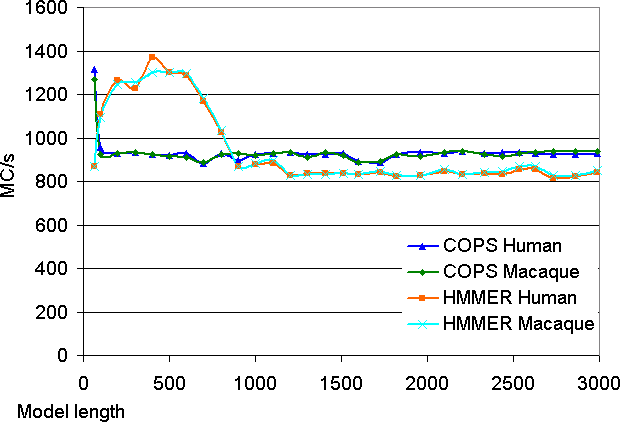
\includegraphics[scale=0.46]{graphics/initial-aleph-runtimes.png}
		\caption[Speeds for the Inter-task vectorization on an AMD Opteron Bulldozer] 
		{Speeds of the initial COPS and HMMER, with the Human and Macaque genomes, on an AMD Opteron Bulldozer.}
		\label{initial-aleph-runtimes}
    \end{minipage}
    \hspace{0.04\linewidth}
    \begin{minipage}{0.48\linewidth}
		\centering
		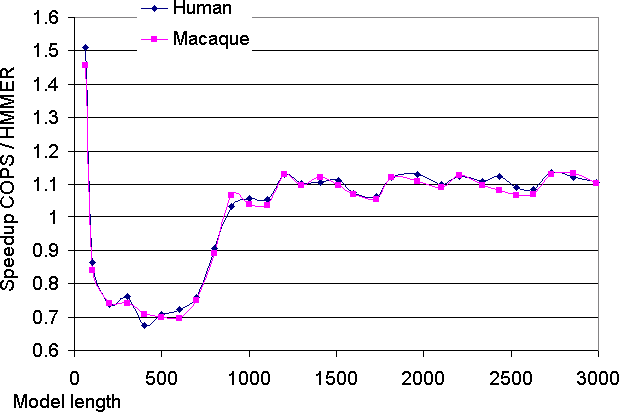
\includegraphics[scale=0.46]{graphics/initial-aleph-speedups.png}
		\caption[Speedups for the Inter-task vectorization on an AMD Opteron Bulldozer] 
		{Speedups of the initial COPS vs HMMER, with the Human and Macaque genomes, on an AMD Opteron Bulldozer.}
		\label{initial-aleph-speedups}
    \end{minipage}
\end{figure} 

\begin{figure}[h!]
    \begin{minipage}{0.48\linewidth}
		\centering
		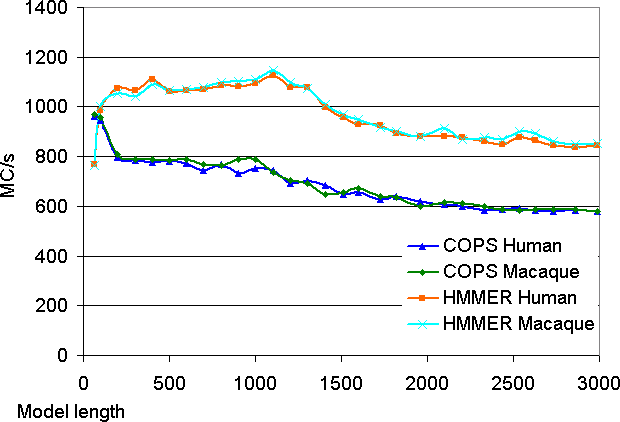
\includegraphics[scale=0.46]{graphics/initial-tags-runtimes.png}
		\caption[Speeds for the Inter-task vectorization on an Intel Xeon Nehalem] 
		{Speeds of the initial COPS and HMMER, with the Human and Macaque genomes, on an Intel Xeon Nehalem.}
		\label{initial-tags-runtimes}
    \end{minipage}
    \hspace{0.04\linewidth}
    \begin{minipage}{0.48\linewidth}
		\centering
		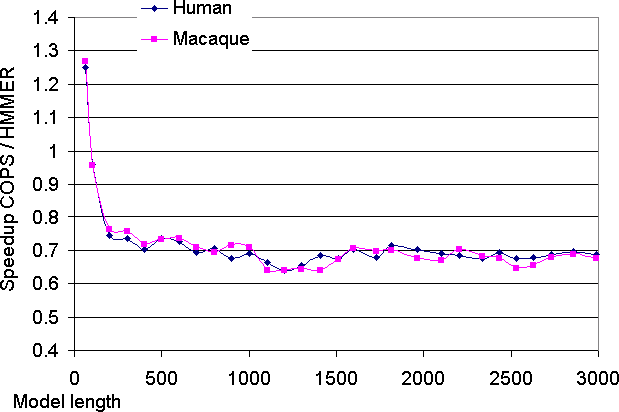
\includegraphics[scale=0.46]{graphics/initial-tags-speedups.png}
		\caption[Speedups for the Inter-task vectorization on an Intel Xeon Nehalem] 
		{Speedups of the initial COPS vs HMMER, with the Human and Macaque genomes, on an Intel Xeon Nehalem.}
		\label{initial-tags-speedups}
    \end{minipage}
\end{figure} 

\begin{figure}[h!]
    \begin{minipage}{0.48\linewidth}
		\centering
		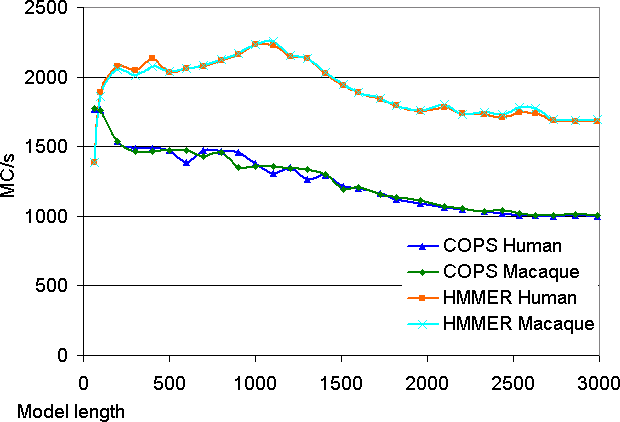
\includegraphics[scale=0.46]{graphics/initial-larissa-runtimes.png}
		\caption[Speeds for the Inter-task vectorization on an Intel i7 Sandy Bridge] 
		{Speeds of the initial COPS and HMMER, with the Human and Macaque genomes, on an Intel i7 Sandy Bridge.}
		\label{initial-larissa-runtimes}
    \end{minipage}
    \hspace{0.04\linewidth}
    \begin{minipage}{0.48\linewidth}
		\centering
		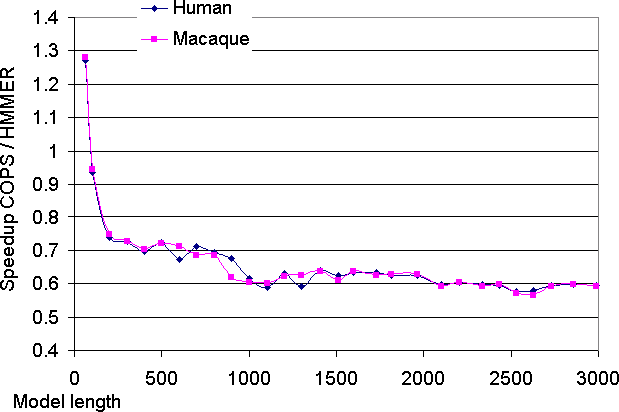
\includegraphics[scale=0.46]{graphics/initial-larissa-speedups.png}
		\caption[Speedups for the Inter-task vectorization on an Intel i7 Sandy Bridge]
		{Speedups of the initial COPS vs HMMER, with the Human and Macaque genomes, on an Intel i7 Sandy Bridge.}
		\label{initial-larissa-speedups}
    \end{minipage}
\end{figure} 

In this section, it is presented the results for the initial approach, based on Rognes' work, whose implementation was described in \sref{Rognes-based SSE Inter-task vectorization}. 

These results show that the original Rognes strategy is not able to surpass the performance of HMMER's ViterbiFilter, except in the case of the smaller models (lengths 60 and 100). From a length-100 model to a lengh-200, the performance of COPS drops drastically, as was discussed in \sref{Problems with First-level Cache Efficiency}.

On the Intel Sandy Bridge a substantial performance drop is also noticeable for larger models ($>$ length-1000). This second drop can also be explained by cache limitations, as it will disappear after normalizing the inner loop maximum memory use (see the later results of \sref{Results for the Model Partitioning}).

In very small models, length $<$ 80 bps, the performance of HMMER's striped version is particularly poor. This poor performance  was equally observed in the Smith-Waterman algorithm. It is caused by the substantial overhead of the Farrar's Lazy-F loop, which is run more frequently (relative to the size of the core computation load) when using very small models. The best results of Rognes' Smith-Waterman program against Farrar's were also found in these smaller lengths (for sequence queries).



\subsection{Results for the Inline loading of the Emission scores}
\label{Results for the Inline loading of the Emission scores}

\begin{figure}[H]
    \begin{minipage}{0.48\linewidth}
		\centering
		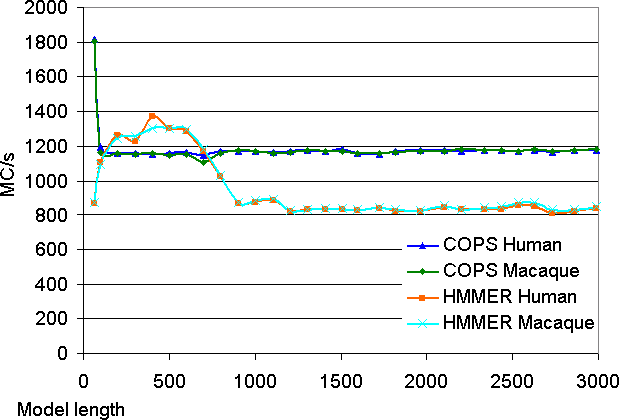
\includegraphics[scale=0.46]{graphics/inlined-aleph-runtimes.png}
		\caption[Speeds of COPS with Inlined Loading and HMMER on an AMD Opteron Bulldozer] 
		{Speeds of COPS with Inlined Loading and HMMER, Human and Macaque genomes, on an AMD Opteron Bulldozer.}
		\label{inlined-aleph-runtimes}
    \end{minipage}
    \hspace{0.04\linewidth}
    \begin{minipage}{0.48\linewidth}
		\centering
		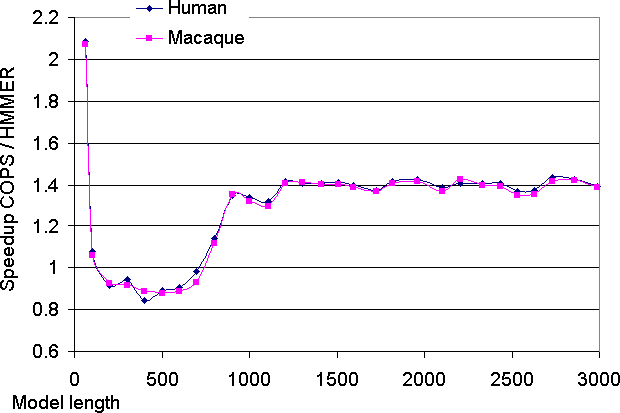
\includegraphics[scale=0.46]{graphics/inlined-aleph-speedups.png}
		\caption[Speedups of COPS with Inlined Loading vs HMMER on an AMD Opteron Bulldozer] 
		{Speedups of COPS with Inlined Loading vs HMMER, Human and Macaque genomes, on an AMD Opteron Bulldozer.}
		\label{inlined-aleph-speedups}
    \end{minipage}
\end{figure} 

\begin{figure}[H]
    \begin{minipage}{0.48\linewidth}
		\centering
		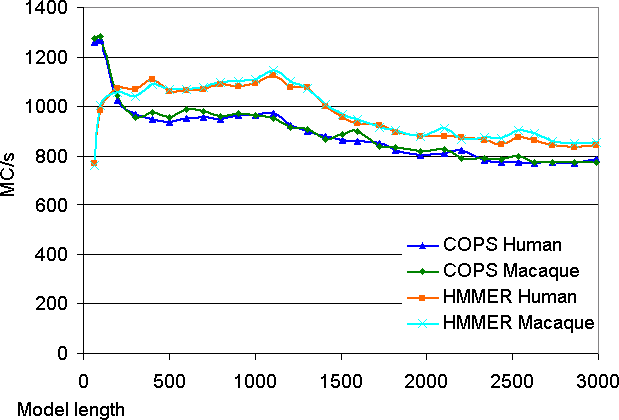
\includegraphics[scale=0.46]{graphics/inlined-tags-runtimes.png}
		\caption[Speeds of COPS with Inlined Loading and HMMER on an Intel Xeon Nehalem] 
		{Speeds of COPS with Inlined Loading and HMMER, Human and Macaque genomes, on an Intel Xeon Nehalem.}
		\label{inlined-tags-runtimes}
    \end{minipage}
    \hspace{0.04\linewidth}
    \begin{minipage}{0.48\linewidth}
		\centering
		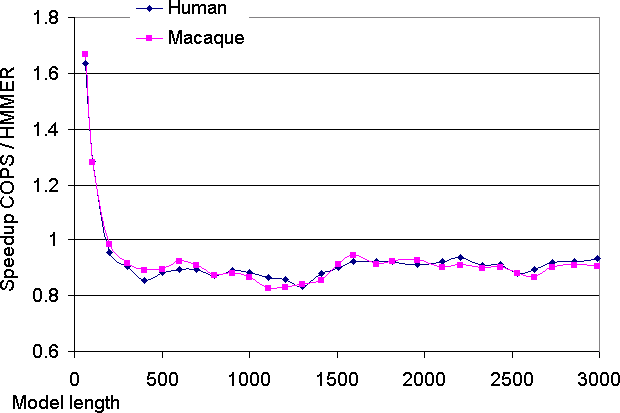
\includegraphics[scale=0.46]{graphics/inlined-tags-speedups.png}
		\caption[Speedups of COPS with Inlined Loading vs HMMER on an Intel Xeon Nehalem] 
		{Speedups of COPS with Inlined Loading vs HMMER, Human and Macaque genomes, on an Intel Xeon Nehalem.}
		\label{inlined-tags-speedups}
    \end{minipage}
\end{figure} 

In this section, Figures 5.7 to 5.12 present the results for the COPS version with the improvement of the loading and arrangement of Emission scores, by inlining the unpack operations in the inner loop. The development of this alternative Inline method was described in \sref{Loading of Emission Scores}. 

With this optimization, there is a general substantial performance boost, between 30\% and 40\% depending on the test machine (see Figures 5.13, 5.14 and 5.15). After this improvement, our COPS tool was able to beat HMMER on some machines (i.e. the AMD Opteron). Still, the performance dependency on model length remained mostly the same. The poor performance of HMMER in the smaller models, and the consequent higher speedup of COPS vs HMMER, remains also unchanged.

\clearpage

\begin{figure}[H]
    \begin{minipage}{0.48\linewidth}
		\centering
		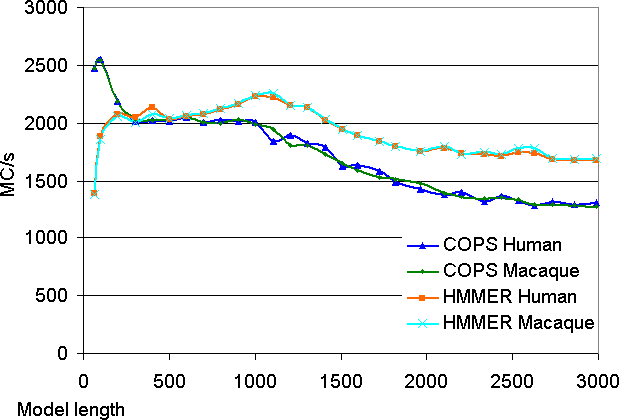
\includegraphics[scale=0.46]{graphics/inlined-larissa-runtimes.png}
		\caption[Speeds of COPS with Inlined Loading and HMMER on an Intel i7 Sandy Bridge] 
		{Speeds of COPS with Inlined Loading and HMMER, Human and Macaque genomes, on an Intel i7 Sandy Bridge.}
		\label{inlined-larissa-runtimes}
    \end{minipage}
    \hspace{0.04\linewidth}
    \begin{minipage}{0.48\linewidth}
		\centering
		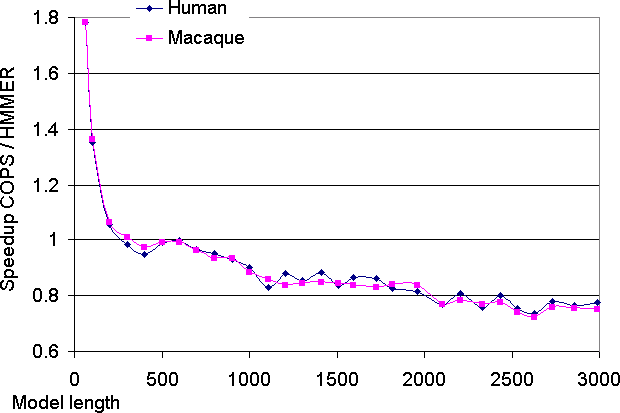
\includegraphics[scale=0.46]{graphics/inlined-larissa-speedups.png}
		\caption[Speedups of COPS with Inlined Loading and HMMER on an Intel i7 Sandy Bridge]
		{Speedups of COPS with Inlined Loading vs HMMER, Human and Macaque genomes, on an Intel i7 Sandy Bridge.}
		\label{inlined-larissa-speedups}
    \end{minipage}
\end{figure} 

\begin{figure}[H]
	\centering
	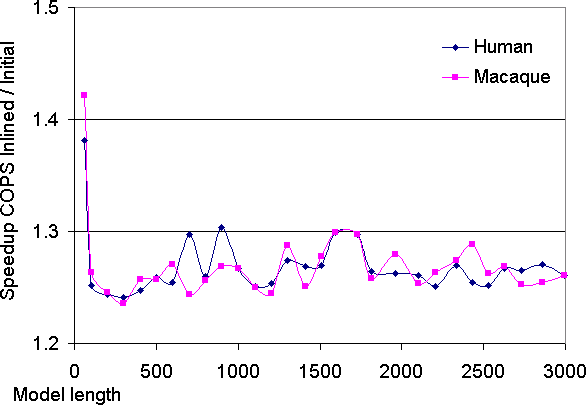
\includegraphics[scale=0.48]{graphics/inlined-cmp-aleph.png}
	\caption[Speedups of Inlined COPS vs Initial COPS on an Intel i7 Sandy Bridge] 
	{Speedups of COPS with Inlined Loading vs Initial COPS, Human and Macaque genomes, on an Intel i7 Sandy Bridge.}
	\label{inlined-cmp-aleph}
\end{figure} 

\begin{figure}[H]
    \begin{minipage}{0.48\linewidth}
		\centering
		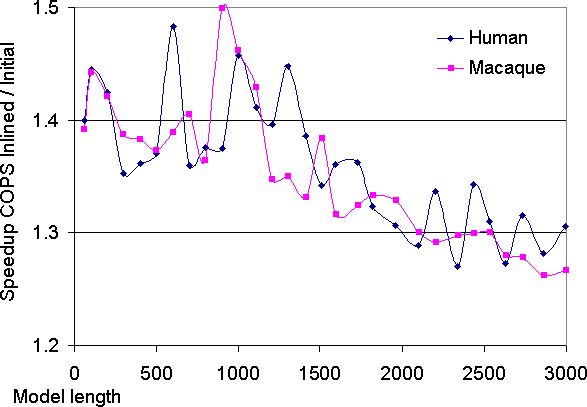
\includegraphics[scale=0.48]{graphics/inlined-cmp-larissa.png}
		\caption[Speedups of Inlined COPS vs Initial COPS on an Intel i7 Sandy Bridge] 
		{Speeds of COPS with Inlined Loading vs Initial COPS, Human and Macaque genomes, on an Intel i7 Sandy Bridge.}
		\label{inlined-cmp-larissa}
    \end{minipage}
    \hspace{0.04\linewidth}
    \begin{minipage}{0.48\linewidth}
		\centering
		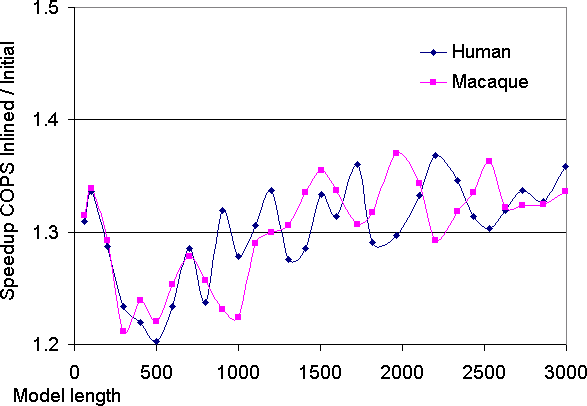
\includegraphics[scale=0.48]{graphics/inlined-cmp-tags.png}
		\caption[Speedups of Inlined COPS vs Initial COPS on an Intel i7 Sandy Bridge]
		{Speedups of COPS with Inlined Loading vs Initial COPS, Human and Macaque genomes, on an Intel i7 Sandy Bridge.}
		\label{inlined-cmp-tags}
    \end{minipage}
\end{figure} 





\subsection{Results for the Model Partitioning}
\label{Results for the Model Partitioning}

\begin{figure}[H]
    \begin{minipage}{0.48\linewidth}
		\centering
		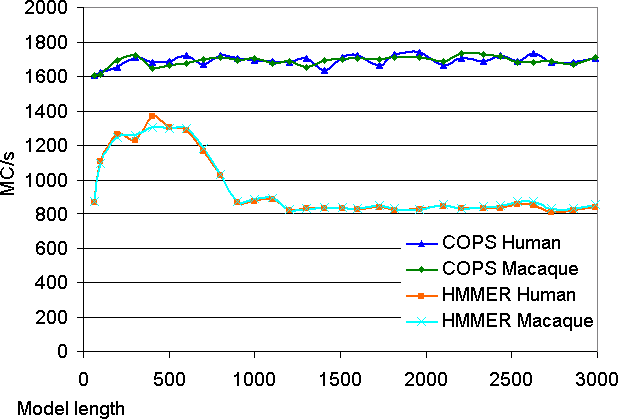
\includegraphics[scale=0.46]{graphics/partitions-aleph-runtimes.png}
		\caption[Speeds for the Inter-task vectorization on an AMD Opteron Bulldozer] 
		{Speeds of COPS after Partitioning and HMMER, with the Human and Macaque genomes, on an AMD Opteron Bulldozer.}
		\label{partitions-aleph-runtimes}
    \end{minipage}
    \hspace{0.04\linewidth}
    \begin{minipage}{0.48\linewidth}
		\centering
		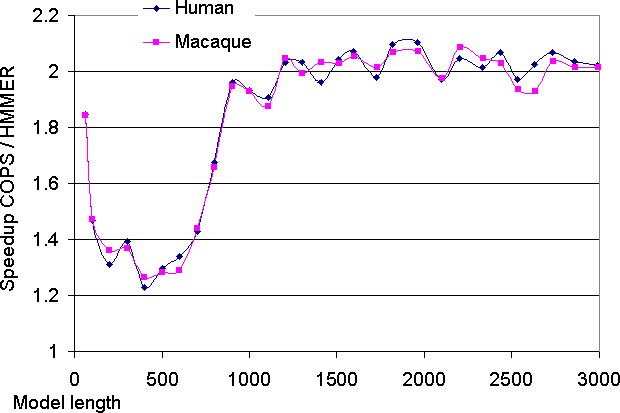
\includegraphics[scale=0.46]{graphics/partitions-aleph-speedups.png}
		\caption[Speedups for the Inter-task vectorization on an AMD Opteron Bulldozer] 
		{Speedups of COPS after Partitioning vs HMMER, with the Human and Macaque genomes, on an AMD Opteron Bulldozer.}
		\label{partitions-aleph-speedups}
    \end{minipage}
\end{figure} 

\begin{figure}[H]
    \begin{minipage}{0.48\linewidth}
		\centering
		\includegraphics[scale=0.46]{graphics/partitions-tags-runtimes.png}
		\caption[Speeds for the Inter-task vectorization on an Intel Xeon Nehalem] 
		{Speeds of COPS after Partitioning and HMMER, with the Human and Macaque genomes, on an Intel Xeon Nehalem.}
		\label{partitions-tags-runtimes}
    \end{minipage}
    \hspace{0.04\linewidth}
    \begin{minipage}{0.48\linewidth}
		\centering
		\includegraphics[scale=0.46]{graphics/partitions-tags-speedups.png}
		\caption[Speedups for the Inter-task vectorization on an Intel Xeon Nehalem] 
		{Speedups of COPS after Partitioning vs HMMER, with the Human and Macaque genomes, on an Intel Xeon Nehalem.}
		\label{partitions-tags-speedups}
    \end{minipage}
\end{figure} 


These are the results for the COPS version after partitioning the HMM model, which has been described in \sref{Model Partitioning to improve the L1 cache utilization}. This evaluated version includes the inline loading of Emission scores.

With model partitioning, the L1 cache size limitation is overcome, and therefore the performance drop from length-100 models to 200-length models, that was evident in the earlier results, disappears. The performance of this version of COPS remains constant with increasing model lengths, in all test machines. 

In particular, this improvement is observed equally in Intel's 32KB L1D cache machines, and in AMD's Opterons with a 16KB L1D cache (see \autoref{partitions-aleph-runtimes}). The optimal partition length was specifically tuned for each test machine (namely, a length of 112-120 for Intel's 32KB caches, and 48 for AMD's 16KB caches). For larger models (length $>$ 1000), COPS is able to beat HMMER on all machines, achieving a speedup ranging from 1.5x on the Intel machines, to 2x on the AMD.

\begin{figure}[h!]
    \begin{minipage}{0.48\linewidth}
		\centering
		\includegraphics[scale=0.46]{graphics/partitions-larissa-runtimes.png}
		\caption[Speeds for the Inter-task vectorization on an Intel i7 Sandy Bridge] 
		{Speeds of COPS after Partitioning and HMMER, with the Human and Macaque genomes, on an Intel i7 Sandy Bridge.}
		\label{partitions-larissa-runtimes}
    \end{minipage}
    \hspace{0.04\linewidth}
    \begin{minipage}{0.48\linewidth}
		\centering
		\includegraphics[scale=0.46]{graphics/partitions-larissa-speedups.png}
		\caption[Speedups for the Inter-task vectorization on an Intel i7 Sandy Bridge]
		{Speedups of COPS after Partitioning vs HMMER, with the Human and Macaque genomes, on an Intel i7 Sandy Bridge.}
		\label{partitions-larissa-speedups}
    \end{minipage}
\end{figure} 

It can be seen in the results that the speedup of COPS vs. HMMER still drops considerably from the smaller M-60 model to the next length-100 model. As referenced before, this drop is explained by the poor showing of HMMER's Viterbifilter in the smaller model. HMMER's striped version executes the \emph{Lazy-F} loop more frequently when the sequence stride is shorter, having a shorter available span to nullify the $F$ dependencies ($D$ for HMMs), and this happens when the model is smaller. Therefore the speedup drop vs. HMMER from the length-60 to the length-100 model is not caused by an efficiency decrease of our version, but by an increase in HMMER. The performance of COPS remains mostly constant in these smaller models, as can be seen in the processing speed graphic.

Therefore, for short models ($<$ 100 bps), COPS achieves a considerable 1.7-fold speedup vs HMMER. For medium-length models (between 200 and 500 bps on 16KB-L1D machines, and up to $\sim$1000 on 32KB-L1D machines), HMMER's implementation is competitive against COPS, reducing our speedup to about 1.2-fold. These are the model lengths wherein the striped version does not exceed the size of the innermost data cache. 

Still, the speedups for short models have not been as high as the ones reported by Rognes for Smith-Waterman. Many reasons may justify this, such as Rognes' aggressive assembly optimizations, and the unavoidable differences between the Viterbi and Smith-Waterman algorithms. One significant cause in our view is the overall higher memory requirements of Viterbi. A inter-task approach is bound to required significantly more memory that an intra-task vectorization, 8-fold for some of the data.

For longer models, from 500 bps or 1000 bps depending on the L1D size, it can be observed that the performance of HMMER quickly deteriorates as the model's length increases, and the memory requirements of the standard Farrar approach reach the maximum that the innermost caches can provide. In contrast, COPS is able to consistently maintain the same performance with increasingly long models, thus achieving a 2-fold speedup on AMD's, and 1.5-fold on Intel's, against HMMER's striped implementation.


The optimized serial benchmark managed a meager result of 228 MC/s on the Core i7, 201 MC/s on the Intel Xeon, and 153MC/s on the AMD, for every model. So, the overall speedup over the non-parallelized code is 11x in the Core i7, 8x on the Intel Xeon, and 8.5x on the AMD.




\subsection{Results for the Wave-Front Multi-threading}
\label{Results for the Wave-Front Multi-threading}

The graphics with the results for the multi-threaded COPS are presented in Appendix A. This version uses a multi-threaded wave-front pattern in the partitions (described in \sref{Multi-threading the partitions}). The evaluation was conducted with an increasing number of threads, 1, 2, 4, 6, and 8 for the 8-core machines.

HMMER's ViterbiFilter is run with independent tasks per thread, in a multi-threaded work pool. Therefore, it is strongly expected that it achieves a quasi-linear speedup over the number of threads, since each thread proceeds independent of the others. The only synchronization point is the access to the work queue, to fetch each new sequence. This synchronization cost is very light - it was measured by comparing against a static work decomposition with same-length sequences (which does not require synchronization primitives), and found to be practically unnoticeable.

The experimental results show that HMMER's Intra-task implementation is able to maintain a linear speedup over the number of threads/scores. This is was the expected outcome, since it is processing each alignment task independently, and there are no inter-thread dependencies (except for the shared work pool).

In the case of COPS, the results show a clear sub-linear speedup, with a considerable drop in the added speed per core, as the number of cores increase. This was also an expected outcome, since there is substantial communication between the threads processing the partitions. Still, other causes may account for some of the lost processing speed. These will be discussed in \sref{Limitations of Wave-Front Multi-threading}. But first, in the next section, the program will be analyzed through Karp-Flatt metric, estimating the serial fraction of the developed program, i.e., the non-parallelized fraction.



\subsection{Evaluation of the experimental serial fraction by Karp-Flatt's Metric}

Karp and Flatt \cite{karpflatt} proposed a metric to measure the portion of a program that is inherently sequential and cannot (or has not) been parallelized - the Experimentally-determined serial fraction ($e$). The metric estimates the value of $e$ by the following formula:

$$ e = \frac{ \displaystyle \frac{1}{Speedup} - \frac{1}{p} } { \displaystyle 1 - \frac{1}{p} } $$

The values derived with this metric from the tests conducted are shown in the graphics below.
%Only the results for the Human genome are presented because the values for the Macaque genome are very close.

\begin{figure}[h!]
    \begin{minipage}{0.48\linewidth}
		\centering
		\includegraphics[scale=0.46]{graphics/karp-flatt-aleph-human.png}
		\caption[Serial fraction on AMD Opteron Bulldozer, Human] {Experimental serial fraction using Karp-Flatt's metric, for the AMD Opteron Bulldozer tests with Human DNA.}
	\label{karp-flatt-aleph-human}
    \end{minipage}
    \hspace{0.04\linewidth}
    \begin{minipage}{0.48\linewidth}
		\centering
		\includegraphics[scale=0.46]{graphics/karp-flatt-aleph-macaque.png}
		\caption[Serial fraction on AMD Opteron Bulldozer, Macaque] {Experimental serial fraction using Karp-Flatt's metric, for the AMD Opteron Bulldozer tests with Macaque DNA.}
	\label{karp-flatt-aleph-macaque}
    \end{minipage}
\end{figure} 

\begin{figure}[h!]
    \begin{minipage}{0.48\linewidth}
		\centering
		\includegraphics[scale=0.46]{graphics/karp-flatt-tags-human.png}
		\caption[Serial fraction on Intel Xeon Nehalem, Human] {Experimental serial fraction using Karp-Flatt's metric, for the Intel Xeon Nehalem tests with Human DNA.}
		\label{karp-flatt-tags-human}
    \end{minipage}
    \hspace{0.04\linewidth}
    \begin{minipage}{0.48\linewidth}
		\centering
		\includegraphics[scale=0.46]{graphics/karp-flatt-tags-macaque.png}
		\caption[Serial fraction on Intel Xeon Nehalem, Macaque] {Experimental serial fraction using Karp-Flatt's metric, for the Intel Xeon Nehalem tests with Macaque DNA.}
		\label{karp-flatt-tags-macaque}
	\end{minipage}
\end{figure} 

\begin{figure}[h!]
    \begin{minipage}{0.48\linewidth}
		\centering
		\includegraphics[scale=0.48]{graphics/karp-flatt-larissa-human.png}
		\caption[Serial fraction on Intel i7 Sandy Bridge, Human] {Experimental serial fraction using Karp-Flatt's metric, for the Intel i7 Sandy Bridge tests with Human DNA.}
		\label{karp-flatt-larissa-human}
    \end{minipage}
    \hspace{0.04\linewidth}
    \begin{minipage}{0.48\linewidth}
		\centering
		\includegraphics[scale=0.48]{graphics/karp-flatt-larissa-macaque.png}
		\caption[Serial fraction on Intel i7 Sandy Bridge, Macaque] {Experimental serial fraction using Karp-Flatt's metric, for the Intel i7 Sandy Bridge tests with Macaque DNA.}
		\label{karp-flatt-larissa-macaque}
	\end{minipage}
\end{figure} 

In general, the serial fraction consistently decreases with the number of threads, in all models, which substantiate the assumption that most of the performance loss is due to the parallel overhead, instead of non-parallelized code. However, there is one exception: in the smaller models (length $<=$ 200), the serial fraction is both considerable higher (indicating a worse parallelization), and it changes little with the number of threads. This result suggests that there is a substantial non-parallelized computation load in these models. That can be explained by the difficulty in finding an optimal work division between partitions and threads, as will be further discussed in the next section.

Another interesting point of note are the wide variations in the serial fraction metric along model lengths, reflecting an efficiency of multi-threading that depends on the specific model length. Some model lengths allow for a perfect work decomposition between partitions and threads, while others do not, and leave some unbalanced workloads. This will also be further discussed in the next section. 

The parallelization had a lower speedup per added thread on the AMD machine than it did on the Intel machines. The different internal architectures of the two different processor families is a likely culprit for this anomaly, since it was found that even a set of independent, non-communicating processes became considerably slower when running concurrently. Additionally, the AMD machine was deployed in a NUMA topology, with a distributed shared memory. The configuration of the DSM seriously hindered any concurrent contention for resources, even among independent processes running on the same NUMA node. 




\subsubsection{Limitations of Wave-Front Multi-threading} 
\label{Limitations of Wave-Front Multi-threading} 

A multi-threading parallelization of the Model partitions, using a wave-front pattern, suffers from some problems that affect its efficiency, and lead to a sub-linear and decreasing parallel speedup:

\begin{itemize}

\item \textbf{Communication overhead}

There are two communication instances between the threads: 
\begin{itemize}[nolistsep]
\item a synchronization point on the flags' arrays, each one shared by only two threads;
\item a data transfer point on partition barriers, which is only accessed before (for writes) and after (for reads) the synchronization point.
\end{itemize}

There is therefore no real contention on the data transfer point, since it is guaranteed to be accessed by only one thread at any given time. The synchronization point suffers some contention from its two owner threads, and the wait cycles when one thread is blocked waiting for the other lead to a non-negligible fraction of thread idle time.


\item \textbf{Start and end delays of the wave-front pattern}

The wave-front pattern entails some unavoidable wait cycles in the start and end of the alignment. Each thread must wait that the previous thread finished the previous partition column, and as a result there is a incremental delay in the beginning, wherein the necessary delay of each thread increases by one work chunk (i.e. one partition column) for each added thread. In the ending of the alignment, the threads that started earlier have to wait for the ones lagging behind, with wait periods in the reserve order.


\item \textbf{Unbalanced work division}

The perfect work division is an even division of the partitions by the threads, and of the model length by the partition length. However it is not always possible to find such a division, especially when the number of threads is higher. The thread work load will become unbalanced in two cases:
\begin{itemize}[nolistsep]
\item When the partitions cannot be evenly distributed by the threads, some thread(s) will get less partitions to process, and will have to wait on the others to finish;
\item When the model length is not evenly divisible by the partition length, the last thread will have less work than the others, and thus will also have to wait. This last unbalanced partition represents a smaller waste than the unbalanced number of partitions, which force thread(s) to wait for the computation period of a whole partition.
\end{itemize}

\item \textbf{Very short partition lengths}

When using partitions that are too small, the various overheads (initialization, termination, synchronization, wave-front delays,  unbalancing idle times, etc) are a large fraction of the overall runtime, due to the corresponding core computation load that has been reduced by the short partition length. These partition lengths should be avoided, but for very small models it may not be possible.

%\item a thread main tem trabalho adicional a preparar a inicializacao, e a extrair os resultados no final => 0.1segs em 84 (fracao)

\end{itemize}
	
The quite noticeable lower speedup per added thread in the smaller models is explained by the uneven load balancing between the threads (some threads have less partitions to compute) and by the heavier overheads when using shorter partition lengths. As more cores are added, the speedup of the wave-front COPS vs HMMER decreases considerably in the smaller models, because the inter-task trivial multi-threading implemented for HMMER's ViterbiFilter does not have these load balancing problems in the test databases (i.e. databases with many sequences).

Conversely, the speedup per added core is higher in the longer models, since they have a better load balancing and a smaller overhead from the longer partitions. Therefore, to effectively exploit the multi-threaded wave-front pattern for a high number of threads (i.e. 8 threads), the application's models should be sufficiently large, in order to reduce the incurred overheads with a close-to-maximum partition length, and achieve an even distribution of partitions among threads.



%\cleardoublepage
\clearpage









%%%%%%%%%%%%%%%%%%%%%%%%%%%%%%%%%%%%%%%%%%%%%%%%%%%%%%%%%%%%%%%%%%%%%%%
%%%%%%%%%%%%%%%%%%%%%%%%%%%%%%%%%%%%%%%%%%%%%%%%%%%%%%%%%%%%%%%%%%%%%%%
%%%%%%%%%%%%%%%%%%%%%%%%%%%%%%%%%%%%%%%%%%%%%%%%%%%%%%%%%%%%%%%%%%%%%%%
	
\fancychapter{Conclusions}

%\section{Dissertation summary}
% resumo do trabalho

Sequence analysis is an increasingly important field in bioinformatics. By comparing biological sequences, proteins and nucleic acids, it is possible to unveil previously unknown relations between different organisms and organelles, such as evolutionary links. This comparison process, known as Homology Search, is a burgeoning field, fueled by the exponential growth of biological data to search. Recent sequencing technology, like Illumina, Pyrosequencing, SOLiD, and others, have greatly expended the quantity of available data that must be analyzed. The biological databases most used for homology search, such as UniProt, TrEMBL, Genbank, etc, have also grown considerably.

Nowadays, two main methods are used to conduct homology search: aligning sequences against each other with tailored alignment algorithms, and evaluating the probability of natural occurrence of a sequence through the use of a probabilistic model, such as a Hidden Markov Model. Both methods have been extensively developed and are in widespread use, offering an invaluable service to biologists. Due to the heavy computational cost of processing the large biological databases that exist today, it has been essential to exploit the enormous potential of hardware parallel computation to speedup the lengthy searches.

Chapter 2 of this thesis expanded on the most relevant algorithms for alignment and Markov Models that are in use today for homology search, along with some important improvements and optimizations of the standard algorithms. Special attention was given to the optimal Smith-Waterman algorithm, which is the basis of many optimization efforts; and to the Viterbi and Forward algorithms for HMMs. Algorithms for single alignment and HMMs were compared and contrasted, focusing particularly on their similarities and common points, as Dynamic Programming algorithms.

Chapter 3 surveyed the major parallelization approaches to Dynamic Programming algorithms (like the Smith-Waterman and Viterbi). The general hardware architectures were covered - SIMD in general purpose CPUs and in GPUs, and MIMD in clusters and multi-core processors. An important distinction was made between intra-task parallelism where a single task is parallelized, and inter-task parallelism which combines multiples tasks to facilitate the parallel work division. 

Three possible decomposition patterns for intra-task parallelism were studied: diagonal, vertical and striped. The striped pattern, first proposed by Farrar, achieved the best speedup and became very popular in many implementations. It is in particular the approach chosen by HMMER, a widely used HMM search tool. In the case of Inter-task parallelism, it was studied the promising work of Rognes in his 2011 Swipe tool. By implementing inter-sequence parallelism on Intel's SSE registers, he managed to surpass Farrar's speedups, for the Smith-Waterman algorithm.

In this work, the objective was to adapt Rognes inter-task strategy to the Viterbi algorithm for HMMs. In particular, to implement it on HMMER and create an alternative Viterbi version that is competitive and surpasses the existing one, which is based on Farrar's pattern. The goal was to reach in HMMER close to the same speedups of around 2.5-fold to 1.5-fold that Rognes achieved against Farrar's version. The development of the work was detailed in Chapter 4.

The inter-sequence vectorization of Viterbi on SSE was successfully implemented, initially following the methods used by Rognes for Smith-Waterman. The performance was clearly lacking however, failing to reach the same processing speed as HMMER's version.
It was then discovered two main issues hindering the program's efficiency: 
\begin{enumerate}
\item The loading and arrangement of the per-sequence Emission Scores;
\item An exhaustion of the available capacity in the innermost L1D cache, in the inner loop code, that happened for medium/large models.
\end{enumerate}

The first issue was tackled by moving the loading of scores into the inner loop, and doing it inlined only 8 vector values at a time. With the inline loading, the values can be kept in close memory and avoid the memory re-writings of Rognes. This improvement led to a speed increase between 30\% and 40\%, shown in the experimental results of \autoref{Results for the Inline loading of the Emission scores}.


The second issue, the L1D cache exhaustion, was solved by dividing the HMM into chunks, which were named partitions. The partitions are then processed in a new outer loop. The inner loop is \emph{strip-mined} so that it processes only one partition in each iteration, as a way to avoid filling the L1D cache capacity. The result was a constant processing speed for any model size, thus making the program \emph{Cache-Oblivious}. For medium and large models, it is faster than HMMER's version, which suffers from the cache encumbrance.


The developed tool, COPS, achieved roughly the same performance as HMMER's ViterbiFilter version on medium models up to $\sim$1000 model states for Intel and $\sim$500 for AMD, and after this threshold, it yielded an increasingly higher speedup against ViterbiFilter. With the larger models, in all benchmarks, COPS obtained speedups between 1.5 and 2.0 against HMMER. The speedups against a serial optimized version ranged from 8-fold to 11-fold.

This advantage in larger models derives mainly from the improved utilization of the innermost cache, that resulted from partitioning the model. By tweaking the maximum partition length (from $\sim$120 for 32KB L1D caches, to $\sim$50 for 16KB caches, and $\sim$220 for 64KB caches), it was possible to maintain an efficient optimal use of the available memory in the L1D cache to store the arrays that are frequently accessed in the inner loop. As a result, it was possible to keep a high performance level when running large models, with which HMMER's ViterbiFilter suffers considerably. We can observe that the performance of HMMER's implementation quickly deteriorates as the model's length increases, and the memory requirements of the standard striped approach reach the maximum that the innermost caches can provide.

For very small models ($<$ $\sim$100 bps), Farrar's approach also suffers considerably due to more passes through the Lazy-F loop. This weakness of Farrar was the main reason behind Rognes' original comparative speedup in his Smith-Waterman program. The same comparative advantage and higher speedup (up to $\sim$1.9-fold) in small models is evident in COPS. 


With this work, we have thus shown that an Inter-task vectorization can effectively improve on Farrar's intra-task striped pattern, and achieve a substantial higher speedup that is independent of the cache size. As such, the developed COPS implementation is a significant improvement on HMMER's implementation.

The comparative speedup obtained against Farrar's approach is higher for very small models, and medium or large models, depending on the machine. Therefore, COPs can be most efficient vis-a-vis a striped pattern in applications that use small models (for instance, most proteins); or large models (such as DNA and RNA analysis, speech and audio recognition, etc).


After developing the single-threaded COPS with the workload divided in partitions, it was explored the avenue of multi-threading parallelization using a wave-front pattern. This consisted in an Intra-task parallelization of each COPS execution, as opposed to an Inter-task trivial parallelization with independent executions. The results were fairly good, as expected, although the parallelization is clearly not scalable for a large number of threads, due to the communication overhead. For a small number of threads however, up to about 8, the obtained speedup through multi-threading is strong, not much lower than a linear speedup (i.e. 6.5-fold speedup for 8 threads). Hence, it has been shown to be an interesting parallelization avenue to employ in some areas. Namely, in the parallelization of very large models that are searched only a few times, and for whom, therefore, the trivial inter-task multi-threading is not very useful due to a lack of independent tasks to divide among threads. 



\section{Main Contributions}

The main contribution of this thesis is the Inter-task vectorization of HMM algorithms. This was successfully accomplished, although the resulting performance did not meet expectations. Two other novel strategies were later developed to improve the original Rognes-based solution. Overall, the main contributions are listed below:

\begin{itemize}
\item Inter-task vectorization of \acp{HMM} algorithms, in commodity CPUs (x86's SSE)

\item Improved method of loading the Emission scores (which correspond to the Match scores of the Smith-Waterman algorithm)

\item Partitioning to Model to fit the inner loops storage arrays in the innermost cache, thus making the program Cache-oblivious

\item Multi-threading the model partitions using a wave-front pattern

\end{itemize}



\section{Future work}

In the author's view, the most promising areas for future work following this thesis are:

\begin{itemize}

\item Adapting the Cache-oblivious model partitioning to Farrar's striped pattern. Although it would surely lead to a performance gain on the larger models, it is expected that it would be lower than the speedup obtained by the Inter-task method. It is my view that the introduction of partitions would make the Lazy-F loop be more frequently executed, which would carry a considerable performance cost. Still, as the partitions would be reasonable large (e.g., $\sim$1000 bps for 32-bit L1D CPUs), the Lazy-F overhead would very likely not nullify the benefits of the reduced L1D cache misses.

\item Adopting and studying the application of the COPS approach in other areas and tools which require Hidden Markov Models, specially those that use larger models, such as speech recognition, DNA analysis, etc. These areas could benefit greatly from an optimized Viterbi implementation.

\item Extending the SSE vectorization to the newest Intel SIMD instruction set, the 256-bit AVX2, which supports operations on 16-bit integers (which AVX1 did not support). Both the Inter-task and the Intra-task striped methods could be ported to AVX2. It is the view of the author that the striped method will obtain a lower speedup than the COPS approach. This expectation is due to the increased frequency of the Lazy-F loop, which happens when the stride is shorter (AVX entails a 2-fold shorter stride for any model length).


\end{itemize}





%%%%%%%%%%%%%%%%%%%%%%%%%%%%%%%%%%%%%%%%%%%%%%%%%%%%%%%%%%%%%%%%%%%%%%
%%%%%%%%%%%%%%%%%%%%%%%%%%%%%%%%%%%%%%%%%%%%%%%%%%%%%%%%%%%%%%%%%%%%%%
%%%%%%%%%%%%%%%%%%%%%%%%%%%%%%%%%%%%%%%%%%%%%%%%%%%%%%%%%%%%%%%%%%%%%%
%%%%%%%%%%%%%%%%%%%%%%%%%%%%%%%%%%%%%%%%%%%%%%%%%%%%%%%%%%%%%%%%%%%%%%



% Add the Bibliography to the PDF table of contents (not the document table of contents)
\pdfbookmark[0]{Bibliography}{bib}
% The bibliography style sheet
% \bibliographystyle{IEEEtran}
\bibliographystyle{apalike}
% \bibliographystyle{unsorted}
% The BiBTeX file
\bibliography{biblio}
\cleardoublepage

\appendix
%\gdef\thesection{Appendix \Alph{section}}

\fancychapter{Code Listings}

\begin{algorithm}[htb!]
\caption[Viterbi algorithm for multihit local alignment] {Pseudo-code of the Viterbi algorithm for multihit local alignment, with the superfluous transitions already removed.}
\label{code-viterbi}

\begin{algorithmic}

\State // Initialization:
\State	$  V^B (0) \gets log\ t_{N B}  $

\For{$i \gets 1 \textrm{ to } SequenceLength \ (L) $} 

	\State	 $ V^M_0(i)  \gets  V^D_0(i)  \gets  V^I_0(i)  \gets  V^E (i)  \gets  -infinity $

	\For{$j  \gets 1  \textrm{ to } ModelSize \ (MS) $} 

		\State	$ V^M_j(i) \gets log \frac{e_{Mj}(x_i) }{q_{xi}} + Max  
				\begin{cases}
					V^B \ (i-1)	    + log\ t_{B_{j-1} M_j} \\
					V^M_{j-1} (i-1) + log\ t_{M_{j-1} M_j}  \\
					V^I_{j-1} (i-1)  + log\ t_{I_{j-1} M_j}  \\
					V^D_{j-1} (i-1) + log\ t_{D_{j-1} M_j} 
				\end{cases} $


		\State	$ V^E_j (i) \gets  Max \begin{cases} 
						V^E_{j-1} (i) \\
						V^M_j(i) \\
						\end{cases} $
	   
		\State	$ V^I_j(i) \gets Max  
				\begin{cases}
					V^M_{j} (i-1) + log\ t_{M_{j} I_j}  \\
					V^I_{j} (i-1) + log\ t_{I_{j} I_j}
				\end{cases} $

		\State	$V^D_j(i) \gets Max \begin{cases}
					V^M_{j-1} (i) + log\ t_{M_{j-1} D_j}  \\
					V^D_{j-1} (i) + log\ t_{D_{j-1} D_j} 
				\end{cases} $ \\

	\EndFor

	
	\State // Updates of special states after the symbol's propagation through all the normal states:
	
	\State	$ V^E_{MS} (i) \gets Max \begin{cases} 
				 V^E_{MS} (i) \\
				 V^M_{MS} (i) \\
				\end{cases} $
	
	\State	$ V^J (i) \gets Max \begin{cases} 
				V^J (i) + log\ t_{J J}  \\
				V^E_{MS} (i) + log\ t_{E J} \\
				\end{cases} $	
					
	\State	$ V^C (i) \gets Max \begin{cases} 
				V^C (i) + log\ t_{C C}  \\
				V^E_{MS} (i) + log\ t_{E C} \\
				\end{cases} $
  
	\State	$ V^N (i) \gets V^N (i-1) + log\ t_{N N} $

	\State	$ V^B (i) \gets Max \begin{cases} 
				V^N (i) + log\ t_{N B}  \\
				V^J (i) + log\ t_{J B} \\
				\end{cases} $	
\EndFor
\end{algorithmic}
\end{algorithm}

\clearpage



\begin{algorithm}[htb!]
\caption[Forward algorithm for multihit local alignment] {Pseudo-code of the Forward algorithm for multihit local alignment, using the Interpolation/Lookup approach, and with the superflous transitions removed. The table $TabLog$ is pre-computed, as well as the logarithmic transition scores $log \; t_{X_j Y_i }$, and emission scores $log \frac{e_{Mj}(x_i) }{q_{xi}} $.}
\label{code-forward}
\begin{algorithmic}

\State // Initialization:
\State	$  F^B (0) \gets log\ t_{N B}  $

\For{$i \gets 1 \textrm{ to } SequenceLength \ (L) $} 

	\State	$ F^M_j(0) = F^D_j(0) = F^I_j(0) = F^E (i) = -infinity $

	\For{$j  \gets 1  \textrm{ to } ModelSize \ (MS) $} 
		\begin{align*}
		 F^M_j(i) = log \frac{e_{Mj}(x_i) }{q_{xi}} + TabLog \;\;  
				[ \ TabLog \ [ \;\; &log\ t_{M_{j-1}M_j} + \; (F^M_{j-1}(i-1)) \ , \\ 
						\;\; &log\ t_{I_{j-1} M_j}  + \; (F^I_{j-1}(i-1)) \ \ ] \ , \\
				TabLog \ [	\;\; &log\ t_{D_{j-1} M_j} + \; (F^D_{j-1}(i-1)) \ , 	\\
						\;\; &log\ t_{B_{j-1} M_j} + \; (F^B (i-1) \ ] \;\; ] 
		\end{align*}
		\begin{align*}
		&F^I_j(i)  \gets TabLog \;\; [ \;\; log\ t_{M_{j} I_j} + \; (F^M_{j}(i-1))  
					     	 + \;\; log\ t_{I_{j} I_j}  + \; (F^I_{j}(i-1))  \;\; ] 
		\\
		&F^D_j(i) \gets TabLog \;\; [ \;\; log\ t_{M_{j} D_j} + \; (F^M_{j-1}(i)) 
					    	  +\;\; log\ t_{M_{j} D_j} + \; (F^D_{j_1}(i))  \;\; ]
		\\
		& F^E_j (i) \gets TabLog \ \ [ F^E_{j-1} (i), TabLog \ [ \ F^M_j(i),  F^D_j(i) \ ] \ ] 
		\end{align*}

	\EndFor
	
	\State \\ Updates of special states after the symbol's propagation through all the normal states:

	\State	$ F^J (i) \gets TabLog \ [\ t_{J J} + F^J(i-1) \ ,  t_{E J} + F^E_{MS} (i) \ ] $

	\State	$ F^C (i) \gets TabLog\ [\ t_{C C} + F^C(i-1) \ ,  t_{E C} + F^E_{MS} (i) \ ] $

	\State	$ F^N (i) \gets log \ t_{N N} + F^N(i-1) $
	
	\State	$ F^B (i) \gets TabLog\ [\ t_{N B} + F^N(i) \ , t_{J B} + F^J(i) \ ] $

\EndFor

\end{algorithmic}
\end{algorithm}

\clearpage


\begin{algorithm}[htb!]
\caption[Initial inner loop code of COPS] {Initial inner loop code of COPS, based on Rognes Smith-Waterman implementation.}
\label{code-rognes}

\begin{algorithmic}
\\
\State $Initialize Mmx, Imx, Dmx to -Vinfinity$

\LeftComment Loop through the sequence symbols
\For {$i \gets 1 \textrm{ to } SequenceLength \ (L) $} 
		
	\State $LoadEmissionScores(e_{match}, i)$

	\State $ xmxE \gets mpv \gets dpv \gets ipv \gets sc \gets dcv \gets -Vinfinity $

	\LeftComment Loop through the model state-triplets
	\For {$i \gets 0 \textrm{ to } M-1 $} 

		\State $ Mnext \gets e_{match}(k) +  VMax
					\begin{cases}
						vB + t_{BM}(k)	\\
						Mpv + t_{MM}(k)	\\
						Ipv + t_{IM}(k)	\\
						Dpv + t_{DM}(k)	\\
					\end{cases} $ \\

		\State $ vE \gets VMax(vE, Mnext) $
		
		\LeftComment Pre-emptive load of M, D, I
		\State $ Dpv \gets Dmx(k) $
		\State $ Ipv  \gets Imx(k)  $
		\State $ Mpv \gets Mmx(k) $

		\LeftComment  Delayed stores of M and D
		\State $ Mmx(k) \gets Mnext $
		\State $ Dmx(k) \gets Dcv   $
		
		\LeftComment Calculate current I(k). $ e_{insert}$  always 0 in HMMER's unilocal mode
		\State $ Imx(k) \gets e_{insert} (k+1) + VMax
					\begin{cases}
						Mpv +  t_{MI}(k+1)	\\
						Ipv +  t_{II}(k+1)		\\
					\end{cases} $ \\

		\LeftComment Calculate next D, D(k+1)
		\State $ Dcv \gets VMax
					\begin{cases}
						Mnext +  t_{MD}(k+1)	\\
						Dcv +  t_{DD}(k+1)	\\
					\end{cases} $ 
	\EndFor
	
	\LeftComment Compute and update the special flanking states
	\State $ vJ  \gets VMAX(vJ + t_{JJ}, vE + t_{EJ})   $	\ \ \ \ \ \ // always 0 for HMMER's Unilocal mode
	\State $ vC \gets VMAX(vC + t_{CC}, vE + t_{EC}) $	\ \ \ \	// $t_{EC}$  is  0 
	\State $ vN \gets vN + t_{NN} $
	\State $ vB \gets VMAX(vN + t_{NM}, vJ + t_{JB})  $	\ \ \ \	// vJ is useless
\EndFor

\end{algorithmic}
\end{algorithm}

\clearpage


\begin{algorithm}[htb!]
\caption[Rognes code to load emission scores] {SSE code of Rognes method to load and arrange the Emission Scores }
\label{code-loading-rognes}

\begin{algorithmic}
\\
\For {$i \gets 1 \textrm{ to } M \textrm{ step }  4 $} 

	\LeftComment Load original scores
	\State	xmm[0] = \_mm\_load\_ps(EMscoreSeq[0]+k)
	\State	xmm[1] = \_mm\_load\_ps(EMscoreSeq[1]+k)
	\State	xmm[2] = \_mm\_load\_ps(EMscoreSeq[2]+k)
	\State xmm[3] = \_mm\_load\_ps(EMscoreSeq[3]+k)
	\LeftComment Interleave 32-bit wide
	\State xmm[4] = \_mm\_unpacklo\_ps(xmm[0], xmm[1])
	\State xmm[5] = \_mm\_unpackhi\_ps(xmm[0], xmm[1])
	\State xmm[6] = \_mm\_unpacklo\_ps(xmm[2], xmm[3])
	\State xmm[7] = \_mm\_unpackhi\_ps(xmm[2], xmm[3])
	\LeftComment Interleave 64-bit wide
	\State xmm[8]   = \_mm\_unpacklo\_pd(xmm[4], xmm[6])
	\State xmm[9]   = \_mm\_unpackhi\_pd(xmm[4], xmm[6])
	\State xmm[10] = \_mm\_unpacklo\_pd(xmm[5], xmm[7])
	\State xmm[11] = \_mm\_unpackhi\_pd(xmm[5], xmm[7])
	\LeftComment Store transposed values
	\State \_mm\_store\_si128(vEmsc+0, xmm[8])
	\State \_mm\_store\_si128(vEmsc+1, xmm[9])
	\State \_mm\_store\_si128(vEmsc+2, xmm[10])
	\State \_mm\_store\_si128(vEmsc+3, xmm[11])
	\State vEmsc = vEmsc + 4
\EndFor
\end{algorithmic}
\end{algorithm}
	
\clearpage




\begin{algorithm}[htb!]
\caption[Inline method code to load emission scores] {SSE code of the Inner loop with the Inline method to load and arrange the Emission Scores }
\label{code-loading-inline}

\begin{algorithmic}
\\
\For {$k \gets 1 \textrm{ to } M \textrm{ step }  4 $} 

	\LeftComment Load original scores
	\State	xmm[0] = \_mm\_load\_ps(EMscoreSeq[0]+k)
	\State	xmm[1] = \_mm\_load\_ps(EMscoreSeq[1]+k)
	\State	xmm[2] = \_mm\_load\_ps(EMscoreSeq[2]+k)
	\State xmm[3] = \_mm\_load\_ps(EMscoreSeq[3]+k)
	\LeftComment Interleave 32-bit wide
	\State xmm[4] = \_mm\_unpacklo\_ps(xmm[0], xmm[1])
	\State xmm[5] = \_mm\_unpackhi\_ps(xmm[0], xmm[1])
	\State xmm[6] = \_mm\_unpacklo\_ps(xmm[2], xmm[3])
	\State xmm[7] = \_mm\_unpackhi\_ps(xmm[2], xmm[3])
	\LeftComment Interleave 64-bit wide
	\State xmm[8]   = \_mm\_unpacklo\_pd(xmm[4], xmm[6])
	\State xmm[9]   = \_mm\_unpackhi\_pd(xmm[4], xmm[6])
	\State xmm[10] = \_mm\_unpacklo\_pd(xmm[5], xmm[7])
	\State xmm[11] = \_mm\_unpackhi\_pd(xmm[5], xmm[7])
	\LeftComment Macro with the inner loop code. Arguments: (model state index, xmm array index)
	\State COMPUTE\_TRIPLET\_STATE(k+0,8)
	\State	COMPUTE\_TRIPLET\_STATE(k+1,9)
	\State COMPUTE\_TRIPLET\_STATE(k+2,10)
	\State	COMPUTE\_TRIPLET\_STATE(k+3,11)
\EndFor
\end{algorithmic}
\end{algorithm}

\clearpage



\begin{algorithm}[h!]
\caption{Pseudo-code of the proposed COPS approach using SSE2 with 8x16-bit integers and saturated arithmetic. This is the final single-threaded version.}
\label{code-complete}

\begin{spacing}{1.08}
\begin{algorithmic}[1]
\item[]
\LeftComment  Loop through the partitions
\For {$p \gets 1 \textrm{ to } Npartitions $} 

	\State $ Initialize \;\; Mmx,\;\;Imx,\;\;Dmx\;\;to\;\; -\infty $

	\LeftComment Loop through the sequence symbols
	\For {$i \gets 1 \textrm{ to } SequenceLength \ (L) $} 
		
		\If { p = 0 }
			\LeftComment First partition, initialize all to $-\infty $
			\State $ xmxE \gets Mnext \gets Dcv \gets -\infty $
		\Else 
			\LeftComment Load data from previous partitions
			\State $xmxE \gets PxmxE(i) $
			\State $Dcv \;\;\; \gets PDcv(i) $
			\State $Mnext   \gets PMnext(i) $
		\EndIf

		\LeftComment Loop through the model state-triplets of the current partition
		\For {$k \gets 0 \textrm{ until } k = PartLength \textrm{ or } 
			 k + p \times PartLength > ModelLength \textrm{ step } 8 $} 
			\LeftComment Load original scores, xmm 0 to 8
			\State	$xmm[0] \gets LOAD16(EMscoreSeq[0]+k) $
			\State	$xmm[1] \gets LOAD32(EMscoreSeq[1]+k) $
			\State ...
			\LeftComment Interleave 16-bit wide, xmm 8 to 15
			\State $xmm[8] \gets UNPACK\_LOW16 (xmm[0], xmm[1]) $
			\State $xmm[9] \gets UNPACK\_HIGH16(xmm[0], xmm[1]) $
			\State ...
			\LeftComment Interleave 32-bit wide, xmm 16 to 23
			\State $xmm[16] \gets UNPACK\_LOW32 (xmm[8], xmm[10]) $
			\State $xmm[17] \gets UNPACK\_HIGH32(xmm[8], xmm[10]) $
			\State ...
			\LeftComment Interleave 64-bit wide, xmm 24 to 31
			\State $xmm[24] \gets UNPACK\_LOW64 (xmm[16], xmm[18) $
			\State $xmm[25] \gets UNPACK\_HIGH64(xmm[16], xmm[18]) $
			\State ...
			\LeftComment Macro with the inner loop code, xmm 24 to 31
			\State $ COMPUTE\_STATE\_TRIPLET(k+0,24) $
			\State	$ COMPUTE\_STATE\_TRIPLET(k+1,25) $
			\State ...
		\EndFor
	
		\LeftComment Compute and update the special flanking states
		\If { $ k + p \times PartLength < ModelLength $ }
			\LeftComment Not the last partiton, store data for next partition
			\State $ PxmxE(i) \gets xmxE $
			\State $ PDcv(i) \gets Dcv $
			\State $ PMnext(i) \gets Mnext $
		\Else 
			\LeftComment Final partition, update the definitive pseudo-states
			\State $ xmxC \gets VMAX16(xmxC, xmxE) $
		\EndIf
	\EndFor
\EndFor

\State \Return $ Undiscretize(VMAX16(xmxC,  t\_{CT})) $
\end{algorithmic}
\end{spacing}
\end{algorithm}

\clearpage



\begin{algorithm}[h!]
\caption{Core inner loop code, used in the macro COMPUTE\_STATE\_TRIPLET(Model State index, Emission Score index). Variable $k$ is the State index}
\label{code-compute}

\begin{algorithmic}[1]
\item[]
\LeftComment Use M value partially computed in last iteration
\State $ Mnext \gets VMAX16
			\begin{cases}
				Mnext \\						
				xmxB + t_{BM}(k)	\\
				xmx[EMindex])
			\end{cases} $ 
\item[]
\item[]
\State $ xmxE \gets VMAX16(vE, Mnext) $		
\item[]
\LeftComment Load scores from last column
\State $ Dpv \gets Dmx(k) $
\State $ Ipv  \gets Imx(k)  $
\State $ Mpv \gets Mmx(k) $
\item[]
\LeftComment Compute and store scores of this column
\State $ Mmx(k) \gets Mnext $
\State $ Dmx(k) \gets Dcv   $

\State $ Imx(k) \gets VMAX16
			\begin{cases}
				Mpv +  t_{MI}(k+1)	\\
				Ipv +  t_{II}(k+1)	\\
			\end{cases} $ 
\item[]
\item[]
\LeftComment Preempetive computation of next-column D score
\State $ Dcv \gets VMAX16
			\begin{cases}
				Mnext +  t_{MD}(k+1)	\\
				Dcv +  t_{DD}(k+1)	\\
			\end{cases} $ 
\item[]
\item[]
\LeftComment Partially compute M score for next column
\State $ Mnext \gets VMAX16
			\begin{cases}
				Mpv + t_{MM}(k)	\\
				Ipv  + t_{IM}(k)	\\
				Dpv + t_{DM}(k)	\\
			\end{cases} $ 
\item[]
\end{algorithmic}
\end{algorithm}
			
\clearpage





\fancychapter{Results of the Wave-Front Multi-threading}

\myparagraph{Wave-Front Multi-threading Results on AMD Opteron Bulldozer} 

\begin{figure}[h!]
    \begin{minipage}{0.48\linewidth}
		\centering
		\includegraphics[scale=0.46]{graphics/threads-aleph-runtimes-human.png}
		\caption[Speeds of the multi-threaded COPS and HMMER, AMD Opteron, Human] 
		{Benchmark speeds of multi-threaded COPS and HMMER, on an AMD Opteron Bulldozer, for the Human genome}
		\label{threads-aleph-runtimes-human}
    \end{minipage}
    \hspace{0.04\linewidth}
    \begin{minipage}{0.48\linewidth}
		\centering
		\includegraphics[scale=0.46]{graphics/threads-aleph-runtimes-macaque.png}
		\caption[Speeds of the multi-threaded COPS and HMMER, AMD Opteron, Macaque] 
		{Benchmark speeds of multi-threaded COPS and HMMER, on an AMD Opteron Bulldozer, for the Macaque genome.}
		\label{threads-aleph-runtimes-macaque}
    \end{minipage}
\end{figure} 

\begin{figure}[h!]
    \begin{minipage}{0.48\linewidth}
		\centering
		\includegraphics[scale=0.46]{graphics/threads-aleph-speedups-human.png}
		\caption[Speedups of the multi-threaded COPS vs HMMER, AMD Opteron, Human] 
		{Benchmark speedups of multi-threaded COPS vs HMMER, on an AMD Opteron Bulldozer, for the Human genome}
		\label{threads-aleph-speedups-human}
    \end{minipage}
    \hspace{0.04\linewidth}
    \begin{minipage}{0.48\linewidth}
		\centering
		\includegraphics[scale=0.46]{graphics/threads-aleph-speedups-macaque.png}
		\caption[Speedups of the multi-threaded COPS vs HMMER, AMD Opteron, Macaque] 
		{Benchmark speedups of multi-threaded COPS vs HMMER, on an AMD Opteron Bulldozer, for the Macaque genome.}
		\label{threads-aleph-speedups-macaque}
    \end{minipage}
\end{figure} 

\clearpage

\myparagraph{Wave-Front Multi-threading Results on Intel Xeon Nehalem} 

\begin{figure}[h!]
    \begin{minipage}{0.48\linewidth}
		\centering
		\includegraphics[scale=0.46]{graphics/threads-tags-runtimes-human.png}
		\caption[Speeds of the multi-threaded COPS and HMMER, Intel Xeon, Human] 
		{Benchmark speeds of multi-threaded COPS and HMMER, on an Intel Xeon Nehalem, for the Human genome}
		\label{threads-tags-runtimes-human}
    \end{minipage}
    \hspace{0.04\linewidth}
    \begin{minipage}{0.48\linewidth}
		\centering
		\includegraphics[scale=0.46]{graphics/threads-tags-runtimes-macaque.png}
		\caption[Speeds of the multi-threaded COPS and HMMER, Intel Xeon, Macaque] 
		{Benchmark speeds of multi-threaded COPS and HMMER, on an Intel Xeon Nehalem, for the Macaque genome.}
		\label{threads-tags-runtimes-macaque}
    \end{minipage}
\end{figure} 

\begin{figure}[h!]
    \begin{minipage}{0.48\linewidth}
		\centering
		\includegraphics[scale=0.46]{graphics/threads-tags-speedups-human.png}
		\caption[Speedups of the multi-threaded COPS vs HMMER, Intel Xeon, Human] 
		{Benchmark speedups of multi-threaded COPS vs HMMER, on an Intel Xeon Nehalem, for the Human genome}
		\label{threads-tags-speedups-human}
    \end{minipage}
    \hspace{0.04\linewidth}
    \begin{minipage}{0.48\linewidth}
		\centering
		\includegraphics[scale=0.46]{graphics/threads-tags-speedups-macaque.png}
		\caption[Speedups of the multi-threaded COPS vs HMMER, Intel Xeon, Macaque] 
		{Benchmark speedups of multi-threaded COPS vs HMMER, on an Intel Xeon Nehalem, for the Macaque genome.}
		\label{threads-tags-speedups-macaque}
    \end{minipage}
\end{figure} 

\clearpage

\myparagraph{Wave-Front Multi-threading Results on Intel Core i7 Sandy Bridge} 

\begin{figure}[h!]
    \begin{minipage}{0.48\linewidth}
		\centering
		\includegraphics[scale=0.46]{graphics/threads-larissa-runtimes-human.png}
		\caption[Speeds of the multi-threaded COPS and HMMER, Intel Core i7, Human] 
		{Benchmark speeds of multi-threaded COPS and HMMER, on an Intel Core i7 Sandy Bridge, for the Human genome}
		\label{threads-larissa-runtimes-human}
    \end{minipage}
    \hspace{0.04\linewidth}
    \begin{minipage}{0.48\linewidth}
		\centering
		\includegraphics[scale=0.46]{graphics/threads-larissa-runtimes-macaque.png}
		\caption[Speeds of the multi-threaded COPS and HMMER, Intel Core i7, Macaque] 
		{Benchmark speeds of multi-threaded COPS and HMMER, on an Intel Core i7 Sandy Bridge, for the Macaque genome.}
		\label{threads-larissa-runtimes-macaque}
    \end{minipage}
\end{figure} 

\begin{figure}[h!]
    \begin{minipage}{0.48\linewidth}
		\centering
		\includegraphics[scale=0.46]{graphics/threads-larissa-speedups-human.png}
		\caption[Speedups of the multi-threaded COPS vs HMMER, Intel Core i7, Human] 
		{Benchmark speedups of multi-threaded COPS vs HMMER, on an Intel Core i7 Sandy Bridge, for the Human genome}
		\label{threads-larissa-speedups-human}
    \end{minipage}
    \hspace{0.04\linewidth}
    \begin{minipage}{0.48\linewidth}
		\centering
		\includegraphics[scale=0.46]{graphics/threads-larissa-speedups-macaque.png}
		\caption[Speedups of the multi-threaded COPS vs HMMER, Intel Core i7, Macaque] 
		{Benchmark speedups of multi-threaded COPS vs HMMER, on an Intel Core i7 Sandy Bridge, for the Macaque genome.}
		\label{threads-larissa-speedups-macaque}
    \end{minipage}
\end{figure} 




\end{document}


